\chapter{First Order Equations}

\noindent
IN THIS CHAPTER we study
first order equations for which there are general methods of
solution.

\medskip\noindent
SECTION~2.1 deals with linear equations, the simplest kind
of first order equations. In this section we introduce the method of
variation of parameters. The idea underlying this method will be a
unifying theme for our approach to solving many different kinds of
differential equations throughout the book.

\medskip\noindent
SECTION~2.2 deals with separable equations, the simplest
nonlinear equations. In this section we introduce the idea of implicit
and constant solutions of differential equations, and we point out
some differences between the properties of linear and nonlinear
equations.

\medskip\noindent
SECTION~2.3 discusses existence and
uniqueness of solutions of nonlinear equations. Although it may seem
logical to place this section before Section~2.2, we
presented
Section~2.2 first so we could have illustrative examples in
Section~2.3.

\medskip\noindent
SECTION~2.4 deals with nonlinear equations that are not
separable, but can be transformed into separable equations by a
procedure similar to variation of parameters.

\medskip\noindent
SECTION~2.5 covers exact differential equations, which are
given this name because the method for solving them uses the idea of
an exact differential from calculus.

\medskip\noindent
SECTION~2.6 deals with
equations that are not exact, but can made exact by multiplying them
by a function known called {\color{blue}\it integrating factor\/}.

\newpage

\section{Linear First Order Equations}

\noindent
A first order differential equation is said to be {\color{blue}\it linear\/} if it can be written as

\begin{equation}
  \label{eq:2.1.1}y'+p(x)y=f(x).
\end{equation}
A first order differential equation that can't be written like this is {\color{blue}\it
nonlinear\/}. We say that \eqref{eq:2.1.1} is {\color{blue}\it homogeneous\/} if $f\equiv0$;
otherwise it's {\color{blue}\it nonhomogeneous\/}. Since $y\equiv0$ is obviously a solution of the
homogeneous equation
\[
  y'+p(x)y=0,
\]
we call it the {\color{blue}\it trivial solution\/}. Any other solution is {\color{blue}\it
nontrivial\/}.

\begin{example}
  \label{example:2.1.1}\rm The first order equations
  \begin{eqnarray*}
    x^{2}y'+3y   & = & x^{2},  \\[2\jot]
    xy'-8x^{2}y  & = & \sin x, \\
    xy'+(\ln x)y & = & 0,      \\
    y'           & = & x^{2}y-2,
  \end{eqnarray*}
  are not in the form \eqref{eq:2.1.1}, but they are linear, since they can be rewritten as
  \begin{eqnarray*}
    y'+\frac{3}{x^{2}}y & = & 1,                \\
    y'-8xy              & = & \frac{\sin x}{x}, \\
    y'+\frac{\ln x}{x}y & = & 0,                \\
    y'-x^{2}y           & = & -2.
  \end{eqnarray*}
\end{example}
% no solution

\begin{example}
  \label{example:2.1.2}\rm Here are some nonlinear first order equations:
  \[
    \begin{array}{rcrc}
      xy'+3y^{2} & = & 2x & \qquad\mbox{(because $y$ is squared)},       \\[2\jot]
      yy'        & = & 3  & \qquad\mbox{(because of the product $yy'$)}, \\[2\jot]
      y'+xe^{y}  & = & 12 & \qquad\mbox{(because of $e^{y}$)}.
    \end{array}
  \]
\end{example}
% no solution

\boxit{General Solution of a Linear First Order Equation}

\noindent
To motivate a definition that we'll need, consider the simple linear first order equation
\begin{equation}
  \label{eq:2.1.2}y'=\frac{1}{x^{2}}.
\end{equation}
From calculus we know that $y$ satisfies this equation if and only if
\begin{equation}
  \label{eq:2.1.3}y=-\frac{1}{x}+c,
\end{equation}
where $c$ is an arbitrary constant. We call $c$ a {\color{blue}\it parameter\/} and say that
\eqref{eq:2.1.3} defines a {\color{blue}\it one--parameter family\/} of functions. For each real
number $c$, the function defined by \eqref{eq:2.1.3} is a solution of \eqref{eq:2.1.2} on
$(-\infty,0)$ and $(0,\infty)$; moreover, every solution of \eqref{eq:2.1.2} on either of these
intervals is of the form \eqref{eq:2.1.3} for some choice of $c$. We say that \eqref{eq:2.1.3} is
{\color{blue}\it the general solution\/} of~\eqref{eq:2.1.2}.

We'll see that a similar situation occurs in connection with any first order linear equation
\begin{equation}
  \label{eq:2.1.4}y'+p(x)y=f(x);
\end{equation}
that is, if $p$ and $f$ are continuous on some open interval $(a,b)$ then there's a unique formula
$y=y(x,c)$ analogous to \eqref{eq:2.1.3} that involves $x$ and a parameter $c$ and has these
properties:
\begin{itemize}
  \item % (a)
    For each fixed value of $c$, the resulting function of $x$ is a solution of \eqref{eq:2.1.4} on
    $(a,b)$.

  \item % (b)
    If $y$ is a solution of \eqref{eq:2.1.4} on $(a,b)$, then $y$ can be obtained from the formula
    by choosing $c$ appropriately.
\end{itemize}
We'll call $y=y(x,c)$ the {\color{blue}\it general solution\/} of \eqref{eq:2.1.4}.

When this has been established, it will follow that an equation of the form
\begin{equation}
  \label{eq:2.1.5}P_{0}(x)y'+P_{1}(x)y=F(x)
\end{equation}
has a general solution on any open interval $(a,b)$ on which $P_{0}$, $P_{1}$, and $F$ are all
continuous and $P_{0}$ has no zeros, since in this case we can rewrite \eqref{eq:2.1.5} in the form
\eqref{eq:2.1.4} with $p=P_{1}/P_{0}$ and $f=F/P_{0}$, which are both continuous on $(a,b)$.

To avoid awkward wording in examples and exercises, we won't specify the interval $(a,b)$ when we
ask for the general solution of a specific linear first order equation. Let's agree that this always
means that we want the general solution on every open interval on which $p$ and $f$ are continuous
if the equation is of the form \eqref{eq:2.1.4}, or on which $P_{0}$, $P_{1}$, and $F$ are
continuous and $P_{0}$ has no zeros, if the equation is of the form \eqref{eq:2.1.5}. We leave it to
you to identify these intervals in specific examples and exercises.

For completeness, we point out that if $P_{0}$, $P_{1}$, and $F$ are all continuous on an open
interval $(a,b)$, but $P_{0}$ {\color{blue}\it does\/} have a zero in $(a,b)$, then \eqref{eq:2.1.5}
may fail to have a general solution on $(a,b)$ in the sense just defined. Since this isn't a major
point that needs to be developed in depth, we won't discuss it further; however, see
Exercise~\ref{exer:2.1.44} for an example.

\boxit{Homogeneous Linear First Order Equations}

\noindent
We begin with the problem of finding the general solution of a homogeneous linear first order
equation. The next example recalls a familiar result from calculus.

\begin{example}
  \label{example:2.1.3} \rm Let $a$ be a constant.
  \begin{alist}
    \item % (a)
    Find the general solution of
    \begin{equation}
      y'-ay=0.\label{eq:2.1.6}
    \end{equation}

    \item % (b)
    Solve the initial value problem
    \[
      y'-ay=0,\quad y(x_{0})=y_{0}.
    \]
  \end{alist}
\end{example}

\begin{examplesolution}
\solutionpart{a} You already know from calculus that if $c$ is any constant, then $y=ce^{ax}$
satisfies \eqref{eq:2.1.6}. However, let's pretend you've forgotten this, and use this problem to
illustrate a general method for solving a homogeneous linear first order equation.

We know that \eqref{eq:2.1.6} has the trivial solution $y\equiv0$. Now suppose $y$ is a nontrivial
solution of \eqref{eq:2.1.6}. Then, since a differentiable function must be continuous, there must
be some open interval $I$ on which $y$ has no zeros. We rewrite \eqref{eq:2.1.6} as
\[
  \frac{y'}{y}=a
\]
for $x$ in $I$. Integrating this shows that
\[
  \ln|y|=ax+k,\mbox{\quad so \quad}|y|=e^{k}e^{ax},
\]
where $k$ is an arbitrary constant. Since $e^{ax}$ can never equal zero, $y$ has no zeros, so $y$ is
either always positive or always negative. Therefore we can rewrite $y$ as
\begin{equation}
  \label{eq:2.1.7}y=ce^{ax}
\end{equation}
where
\[
  c=\left\{
  \begin{array}{cl}
    \phantom{-}e^{k} & \mbox{if }y>0, \\
    -e^{k}           & \mbox{if }y<0.
  \end{array}\right.
\]
This shows that every nontrivial solution of \eqref{eq:2.1.6} is of the form $y=ce^{ax}$ for some
nonzero constant $c$. Since setting $c=0$ yields the trivial solution, {\color{blue}\it all\/}
solutions of \eqref{eq:2.1.6} are of the form \eqref{eq:2.1.7}. Conversely, \eqref{eq:2.1.7} is a
solution of \eqref{eq:2.1.6} for every choice of $c$, since differentiating \eqref{eq:2.1.7} yields
$y'=ace^{ax}=ay$.

\solutionpart{b} Imposing the initial condition $y(x_{0})=y_{0}$ yields $y_{0}=ce^{ax_{0}}$, so
$c=y_{0}e^{-ax_{0}}$ and
\[
  y=y_{0}e^{-ax_{0}}e^{ax}=y_{0}e^{a(x-x_{0})}.
\]
Figure~\ref{figure:2.1.1} shows the graphs of this function with $x_{0}=0$, $y_{0}=1$, and various
values of $a$.

\begin{figure}[tbp]
  \centering
  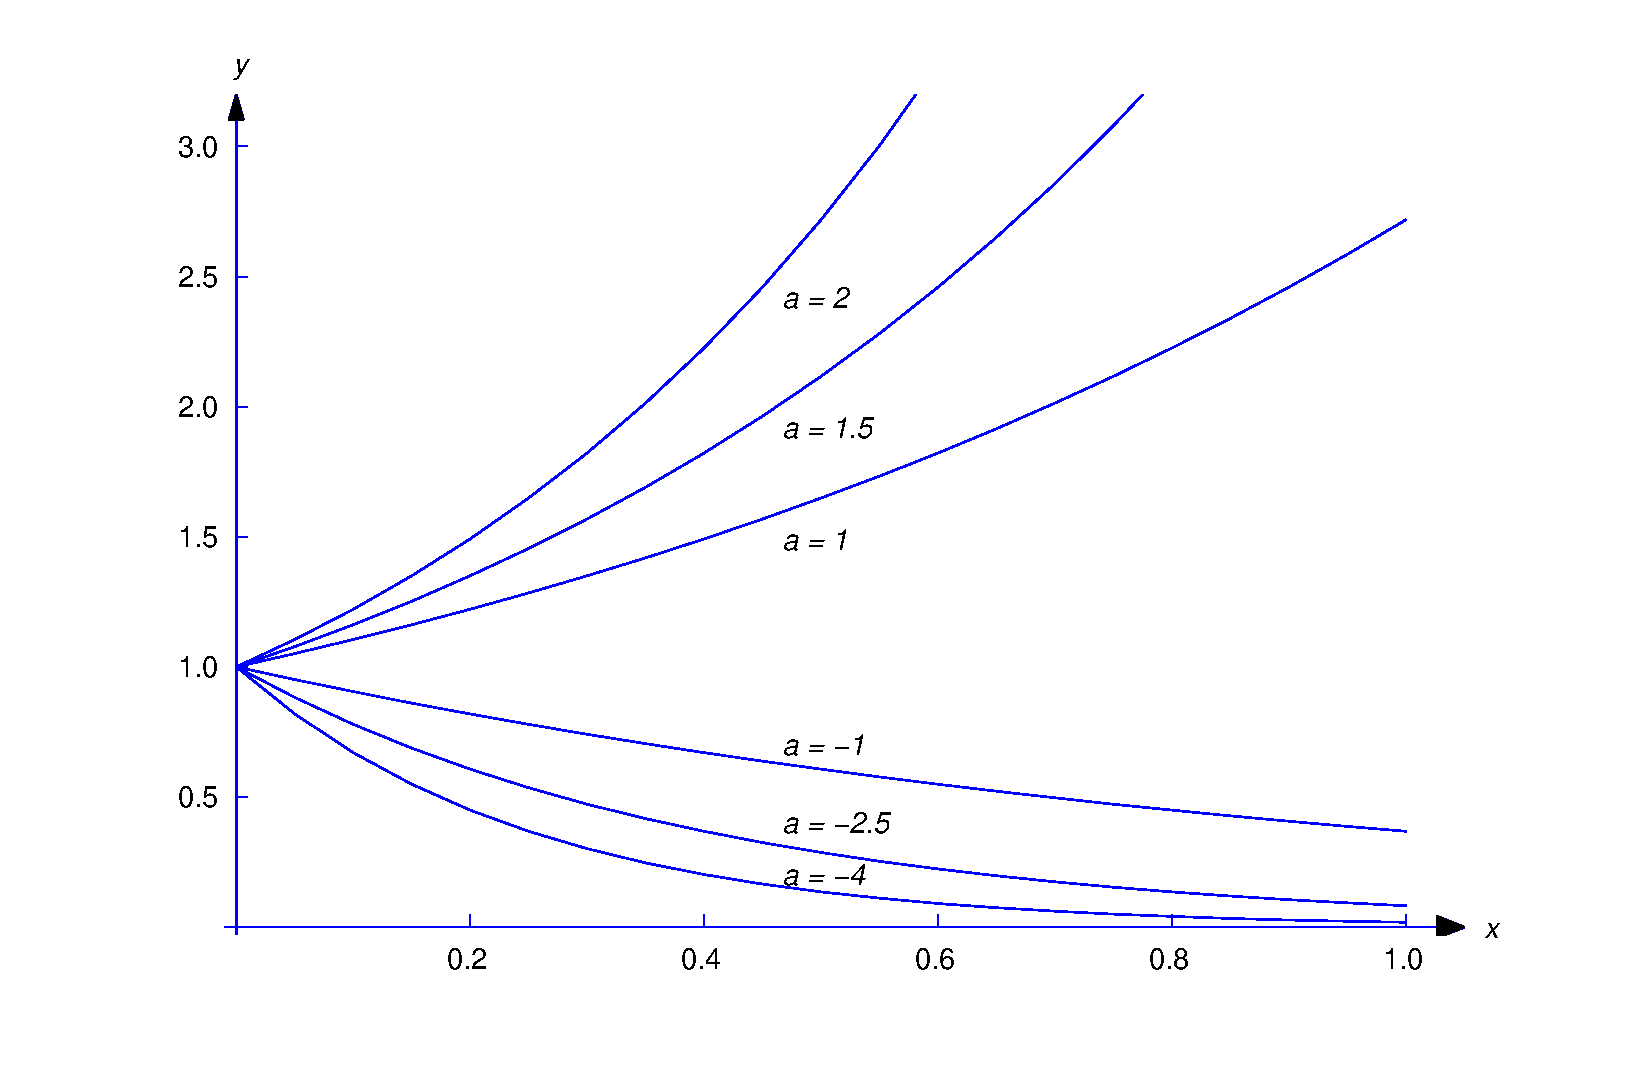
\includegraphics[bb=-78 148 689 643, width=5.67in, height=3.66in, keepaspectratio]{fig020101}
  \color{blue}
  \caption{Solutions of $y'-ay=0$, $y(0)=1$}
  \label{figure:2.1.1}
\end{figure}
\end{examplesolution}

\begin{example}
  \label{example:2.1.4}\rm

  \begin{alist}
    \item % (a)
    Find the general solution of
    \begin{equation}
      xy'+y=0.\label{eq:2.1.8}
    \end{equation}

    \item % (b)
    Solve the initial value problem
    \begin{equation}
      xy'+y=0,\quad y(1)=3.\label{eq:2.1.9}
    \end{equation}
  \end{alist}
\end{example}

\begin{examplesolution}
\solutionpart{a} We rewrite \eqref{eq:2.1.8} as
\begin{equation}
  \label{eq:2.1.10}y'+\frac{1}{x}y=0,
\end{equation}
where $x$ is restricted to either $(-\infty,0)$ or $(0,\infty)$. If $y$ is a nontrivial solution of
\eqref{eq:2.1.10}, there must be some open interval I on which $y$ has no zeros. We can rewrite
\eqref{eq:2.1.10} as
\[
  \frac{y'}{y}=-\frac{1}{x}
\]
for $x$ in $I$. Integrating shows that
\[
  \ln|y|=-\ln|x|+k,\mbox{\quad so\quad}|y|=\frac{e^{k}}{|x|}.
\]
Since a function that satisfies the last equation can't change sign on either $(-\infty,0)$ or
$(0,\infty)$, we can rewrite this result more simply as
\begin{equation}
  \label{eq:2.1.11}y=\frac{c}{x}
\end{equation}
where
\[
  c=\left\{
  \begin{array}{cl}
    \phantom{-}e^{k} & \mbox{if }y>0, \\
    -e^{k}           & \mbox{if }y<0.
  \end{array}\right.
\]
We've now shown that every solution of \eqref{eq:2.1.10} is given by \eqref{eq:2.1.11} for some
choice of $c$. (Even though we assumed that $y$ was nontrivial to derive \eqref{eq:2.1.11}, we can
get the trivial solution by setting $c=0$ in \eqref{eq:2.1.11}.) Conversely, any function of the
form \eqref{eq:2.1.11} is a solution of \eqref{eq:2.1.10}, since differentiating \eqref{eq:2.1.11}
yields
\[
  y'=-\frac{c}{x^{2}},
\]
and substituting this and \eqref{eq:2.1.11} into \eqref{eq:2.1.10} yields
\begin{eqnarray*}
  y'+\frac{1}{x}y & = & -\frac{c}{x^{2}}+\frac{1}{x}\frac{c}{x} \\[2\jot]
                  & = & -\frac{c}{x^{2}}+\frac{c}{x^{2}}=0.
\end{eqnarray*}

Figure~\ref{figure:2.1.2} shows the graphs of some solutions corresponding to various values of $c$. \solutionpart{b} Imposing the initial condition $y(1)=3$ in \eqref{eq:2.1.11} yields $c=3$.
Therefore the solution of \eqref{eq:2.1.9} is
\[
  y=\frac{3}{x}.
\]
The interval of validity of this solution is $(0,\infty)$.

\begin{figure}[tbp]
  \centering
  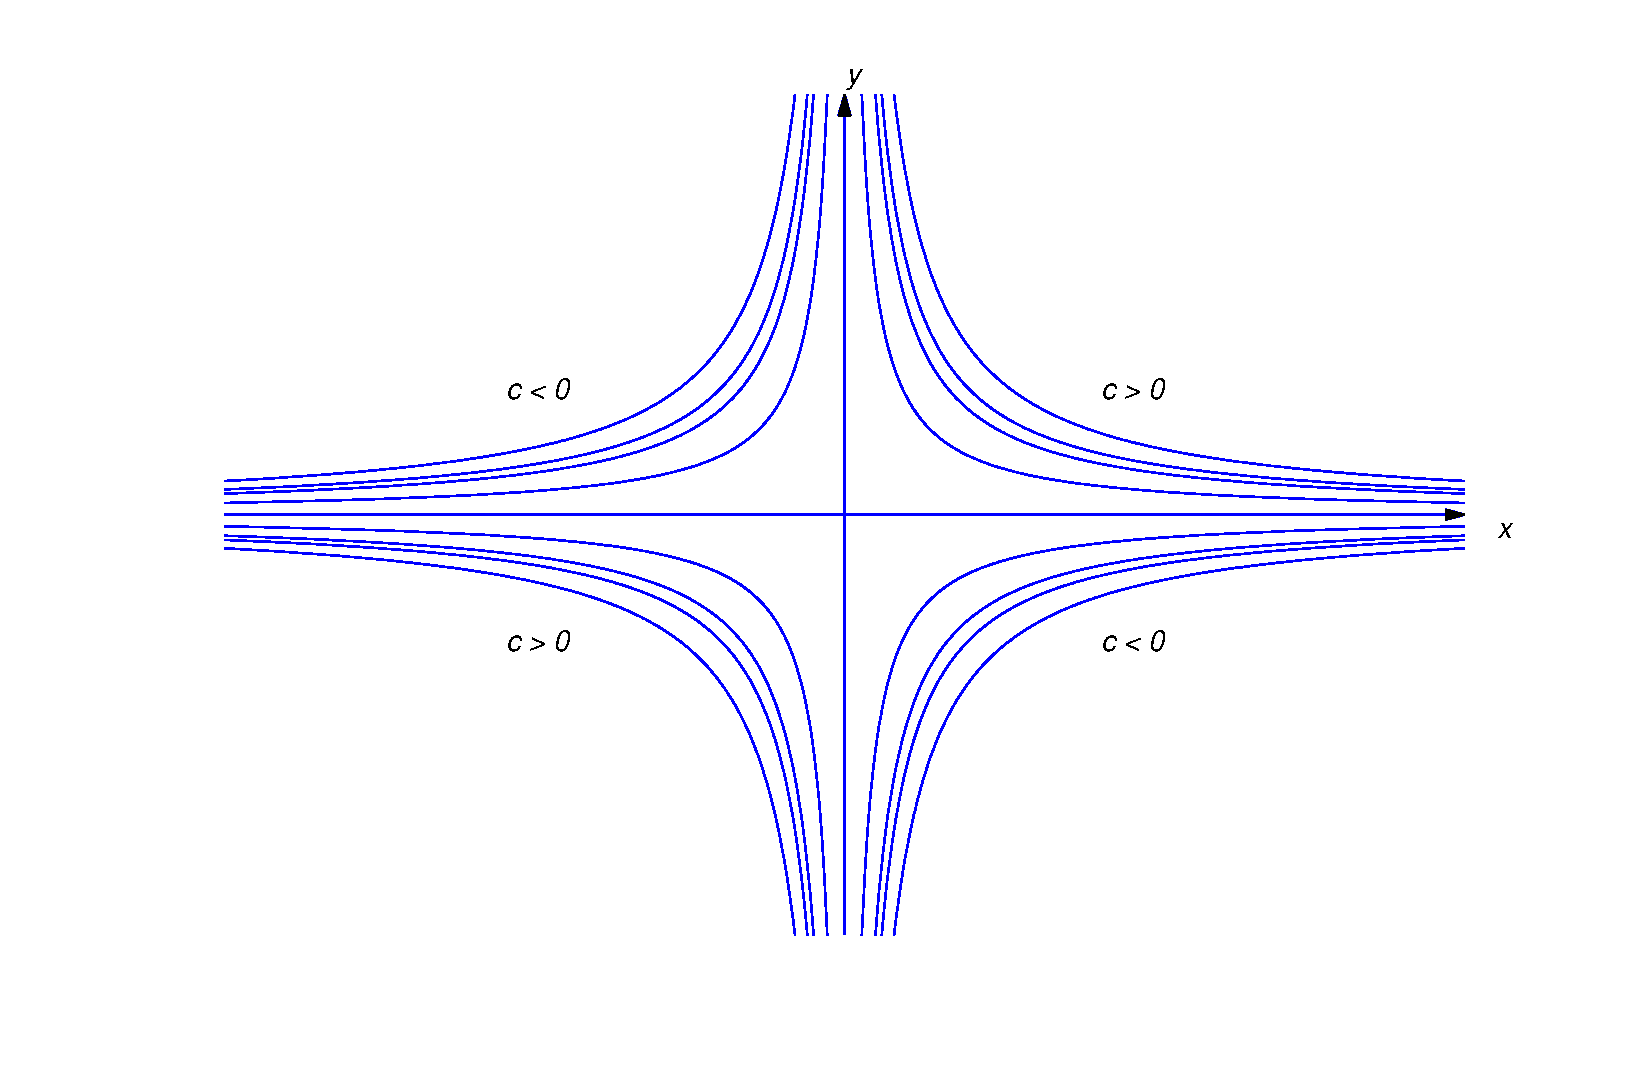
\includegraphics[bb=-78 148 689 643, width=5.67in, height=3.66in, keepaspectratio]{fig020102}
  \color{blue}
  \caption{Solutions of $xy'+y=0$ on $(0,\infty)$ and $(-\infty,0)$}
  \label{figure:2.1.2}
\end{figure}
\end{examplesolution}

The results in Examples~\ref{example:2.1.3}\part{a} and \ref{example:2.1.4}\part{a} are special
cases of the next theorem.

\begin{theorem}
  \color{blue}
  \label{thmtype:2.1.1} If $p$ is continuous on $(a,b)$, then the general solution of the
  homogeneous equation
  \begin{equation}
    \label{eq:2.1.12}y'+p(x)y=0
  \end{equation}
  on $(a,b)$ is
  \[
    y=ce^{-P(x)},
  \]
  where
  \begin{equation}
    \label{eq:2.1.13}P(x)=\int p(x)\,dx
  \end{equation}
  is any antiderivative of $p$ on $(a,b)$; that is,
  \begin{equation}
    \label{eq:2.1.14}P'(x)=p(x),\quad a<x<b.
  \end{equation}
\end{theorem}

\proof If $y=ce^{-P(x)}$, differentiating $y$ and using \eqref{eq:2.1.14} shows that
\[
  y'=-P'(x)ce^{-P(x)}=-p(x)ce^{-P(x)}=-p(x)y,
\]
so $y'+p(x)y=0$; that is, $y$ is a solution of \eqref{eq:2.1.12}, for any choice of $c$.

Now we'll show that any solution of \eqref{eq:2.1.12} can be written as $y=ce^{-P(x)}$ for some
constant $c$. The trivial solution can be written this way, with $c=0$. Now suppose $y$ is a
nontrivial solution. Then there's an open subinterval $I$ of $(a,b)$ on which $y$ has no zeros. We
can rewrite \eqref{eq:2.1.12} as
\begin{equation}
  \label{eq:2.1.15}\frac{y'}{y}=-p(x)
\end{equation}
for $x$ in $I$. Integrating \eqref{eq:2.1.15} and recalling \eqref{eq:2.1.13} yields
\[
  \ln|y|=-P(x)+k,
\]
where $k$ is a constant. This implies that
\[
  |y|=e^{k}e^{-P(x)}.
\]
Since $P$ is defined for all $x$ in $(a,b)$ and an exponential can never equal zero, we can take
$I=(a,b)$, so $y$ has no zeros on $(a,b)$, so we can rewrite the last equation as
$y=ce^{-P(x)}$, where
\[
  c=\left\{
  \begin{array}{cl}
    \phantom{-}e^{k} & \mbox{if }y>0\mbox{ on } (a,b), \\
    -e^{k}           & \mbox{if }y<0\mbox{ on }(a,b).
  \end{array}\right.
\]

\color{blue}
\remark{Rewriting a first order differential equation so that one side depends only on $y$ and $y'$
and the other depends only on $x$ is called {\color{blue}\it separation of variables\/}. We did this
in Examples~ \ref{example:2.1.3} and \ref{example:2.1.4}, and in rewriting \eqref{eq:2.1.12} as
\eqref{eq:2.1.15}. We'll apply this method to nonlinear equations in Section~2.2.}
\color{black}

\boxit{Linear Nonhomogeneous First Order Equations}

\noindent
We'll now solve the nonhomogeneous equation
\begin{equation}
  \label{eq:2.1.16}y'+p(x)y=f(x).
\end{equation}
When considering this equation we call
\[
  y'+p(x)y=0
\]
the {\color{blue}\it complementary equation}.

We'll find solutions of \eqref{eq:2.1.16} in the form $y=uy_{1}$, where $y_{1}$ is a nontrivial
solution of the complementary equation and $u$ is to be determined. This method of using a solution
of the complementary equation to obtain solutions of a nonhomogeneous equation is a special case of
a method called {\color{blue}\it variation of parameters\/}, which you'll encounter several times in
this book. (Obviously, $u$ can't be constant, since if it were, the left side of \eqref{eq:2.1.16}
would be zero. Recognizing this, the early users of this method viewed $u$ as a ``parameter'' that
varies; hence, the name ``variation of parameters.'')

If
\[
  y=uy_{1},\mbox{\quad then\quad}y'=u'y_{1}+uy_{1}'.
\]
Substituting these expressions for $y$ and $y'$ into \eqref{eq:2.1.16} yields
\[
  u'y_{1}+u(y_{1}'+p(x)y_{1})=f(x),
\]
which reduces to
\begin{equation}
  \label{eq:2.1.17}u'y_{1}=f(x),
\end{equation}
since $y_{1}$ is a solution of the complementary equation; that is,
\[
  y_{1}'+p(x)y_{1}=0.
\]
In the proof of Theorem~\ref{thmtype:2.1.1} we saw that $y_{1}$ has no zeros on an interval where
$p$ is continuous. Therefore we can divide \eqref{eq:2.1.17} through by $y_{1}$ to obtain
\[
  u'=f(x)/y_{1}(x).
\]
We can integrate this (introducing a constant of integration), and multiply the result by $y_{1}$ to
get the general solution of \eqref{eq:2.1.16}. Before turning to the formal proof of this claim,
let's consider some examples.

\begin{example}
  \label{example:2.1.5}\rm Find the general solution of
  \begin{equation}
    \label{eq:2.1.18}y'+2y=x^{3}e^{-2x}.
  \end{equation}
\end{example}

\begin{examplesolution}
\solution By applying \part{a} of Example~ \ref{example:2.1.3} with $a=-2$, we see that $y_{1}=e^{-2x}$ is a
solution of the complementary equation $y'+2y=0$. Therefore we seek solutions of \eqref{eq:2.1.18}
in the form $y=ue^{-2x}$, so that
\begin{equation}
  \label{eq:2.1.19}y'=u'e^{-2x}-2ue^{-2x}\mbox{\quad and \quad }y'+2y=u'e^{-2x}-2ue^{-2x}+2ue^{-2x}=u'e^{-2x}.
\end{equation}
Therefore $y$ is a solution of \eqref{eq:2.1.18} if and only if
\[
  u'e^{-2x}=x^{3}e^{-2x}\mbox{\quad or, equivalently,\quad}u'=x^{3}.
\]
Therefore
\[
  u=\frac{x^{4}}{4}+c,
\]
and
\[
  y=ue^{-2x}=e^{-2x}\left(\frac{x^{4}}{4}+c\right)
\]
is the general solution of \eqref{eq:2.1.18}.

Figure~\ref{figure:2.1.3} shows a direction field and some integral curves for \eqref{eq:2.1.18}.

\begin{figure}[tbp]
  \centering
  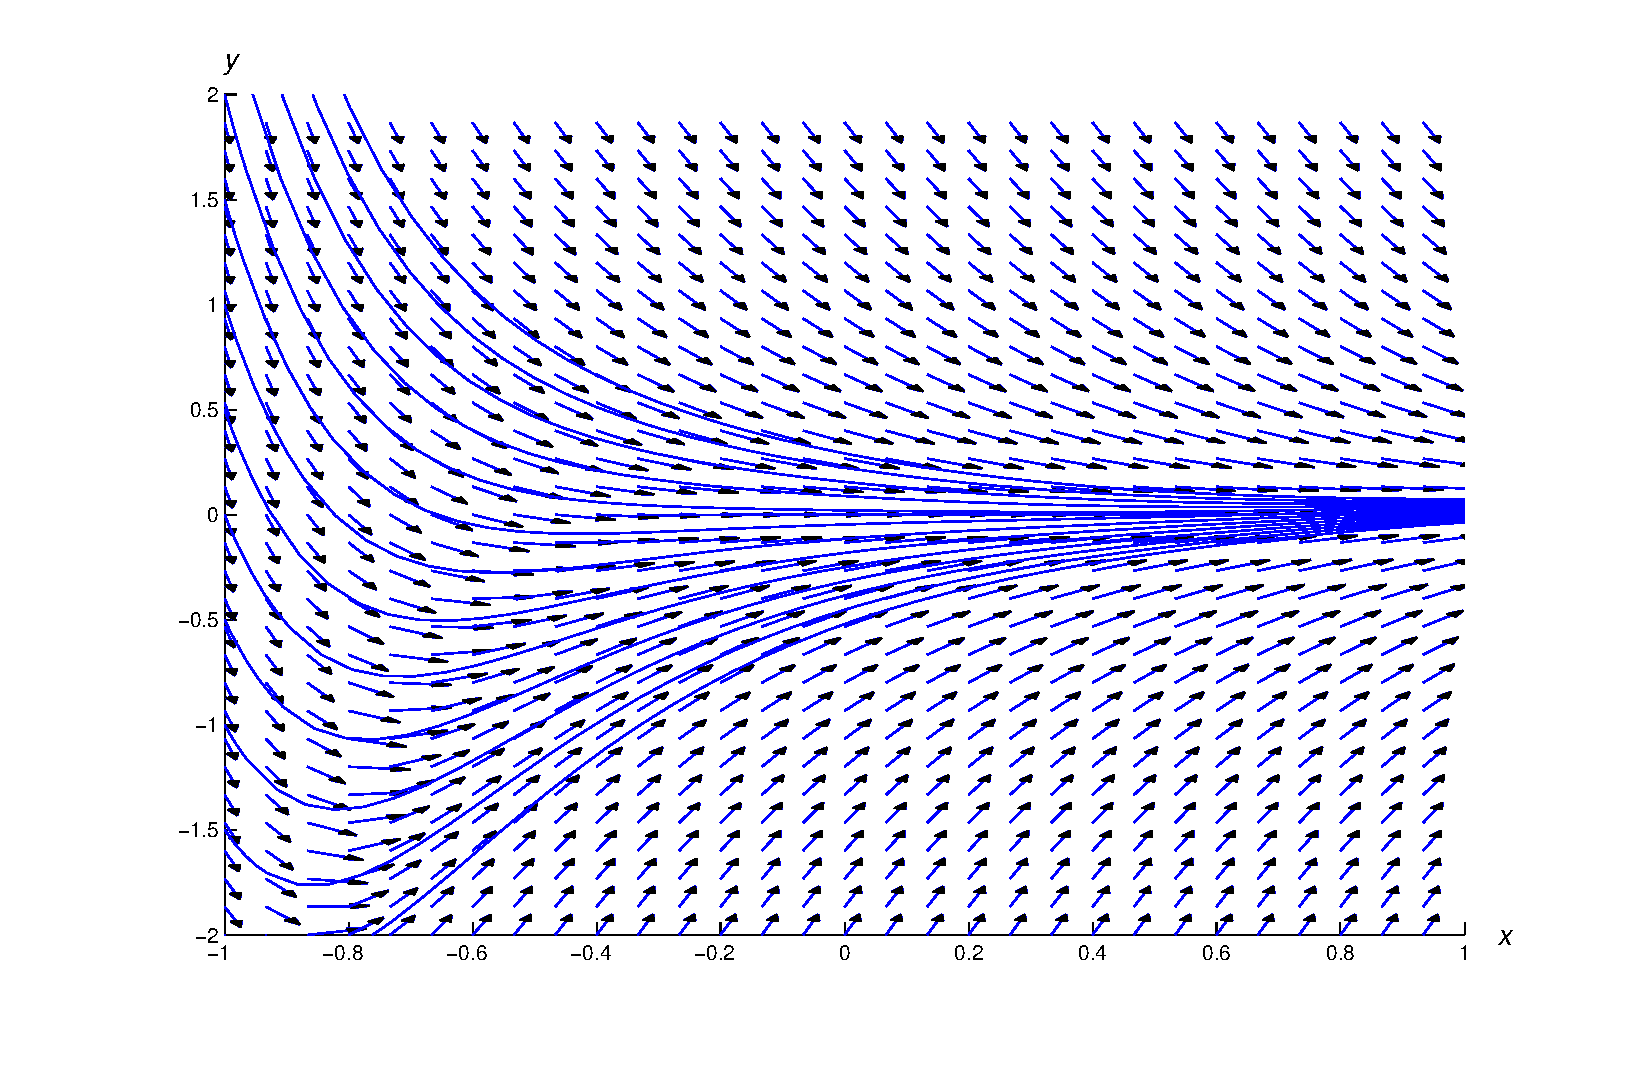
\includegraphics[bb=-78 148 689 643, width=5.67in, height=3.66in, keepaspectratio]{fig020103}
  \color{blue}
  \caption{A direction field and integral curves for $y'+2y=x^{3}e^{-2x}$}
  \label{figure:2.1.3}
\end{figure}
\end{examplesolution}

\begin{example}
  \label{example:2.1.6}\rm\mbox{}%\newline
  \begin{alist}
    \item % (a)
    Find the general solution
    of \begin{equation}
      \label{eq:2.1.20}y'+(\cot x)y=x\csc x.
    \end{equation}

    \item % (b)
    Solve the initial value problem
    \begin{equation}
      \label{eq:2.1.21}y'+(\cot x)y=x\csc x,\quad y(\pi/2)=1.
    \end{equation}
  \end{alist}
\end{example}

\begin{examplesolution}
\solutionpart{a} Here $p(x)=\cot x$ and $f(x)=x\csc x$ are both continuous except at the points
$x=r\pi$, where $r$ is an integer. Therefore we seek solutions of \eqref{eq:2.1.20} on the intervals
$\left(r\pi,(r+1)\pi\right)$. We need a nontrivial solution $y_{1}$ of the complementary equation;
thus, $y_{1}$ must satisfy $y_{1}'+(\cot x)y_{1}=0$, which we rewrite as
\begin{equation}
  \label{eq:2.1.22}\frac{y_{1}'}{y_{1}}=-\cot x=-\frac{\cos x}{\sin x}.
\end{equation}
Integrating this yields
\[
  \ln|y_{1}|=-\ln|\sin x|,
\]
where we take the constant of integration to be zero since we need only {\color{blue}\it one\/}
function that satisfies \eqref{eq:2.1.22}. Clearly $y_{1}=1/\sin x$ is a suitable choice. Therefore
we seek solutions of \eqref{eq:2.1.20} in the form
\[
  y=\frac{u}{\sin x},
\]
so that
\begin{equation}
  \label{eq:2.1.23}y'=\frac{u'}{\sin x}-\frac{u\cos x}{\sin^{2}x}
\end{equation}
and
\begin{equation}
  \label{eq:2.1.24}
  \begin{array}{rcl}
    y'+(\cot x)y & = & \dst\frac{u'}{\sin x}-\dst\frac{u\cos x}{\sin^{2}x}+\dst\frac{u\cot x}{\sin x}    \\[2\jot]
                 & = & \dst\frac{u'}{\sin x}-\dst\frac{u\cos x}{\sin^{2}x}+\dst\frac{u\cos x}{\sin^{2}x} \\[2\jot]
                 & = & \dst\frac{u'}{\sin x}.
  \end{array}
\end{equation}
Therefore $y$ is a solution of \eqref{eq:2.1.20} if and only if
\[
  u'/\sin x=x\csc x=x/\sin x\mbox{\quad or, equivalently, \quad}u'=x.
\]
Integrating this yields
\begin{equation}
  \label{eq:2.1.25}u=\frac{x^{2}}{2}+c,\text{\quad and \quad }y=\frac{u}{\sin x}=\frac{x^{2}}{2\sin x}+\frac{c}{\sin x}
\end{equation}
is the general solution of \eqref{eq:2.1.20} on every interval $\left(r\pi,(r+1)\pi\right)$
($r=$integer).

\solutionpart{b} Imposing the initial condition $y(\pi/2)=1$ in \eqref{eq:2.1.25} yields
\[
  1=\frac{\pi^{2}}{8}+c\mbox{\quad or\quad}c=1-\frac{\pi^{2}}{8}.
\]
Thus,
\[
  y=\frac{x^{2}}{2\sin x}+\frac{(1-\pi^{2}/8)}{\sin x}
\]
is a solution of \eqref{eq:2.1.21}. The interval of validity of this solution is $(0,\pi)$;
Figure~\ref{figure:2.1.4} shows its graph.

\begin{figure}[H]
  \centering
  \scalebox{.8}{
  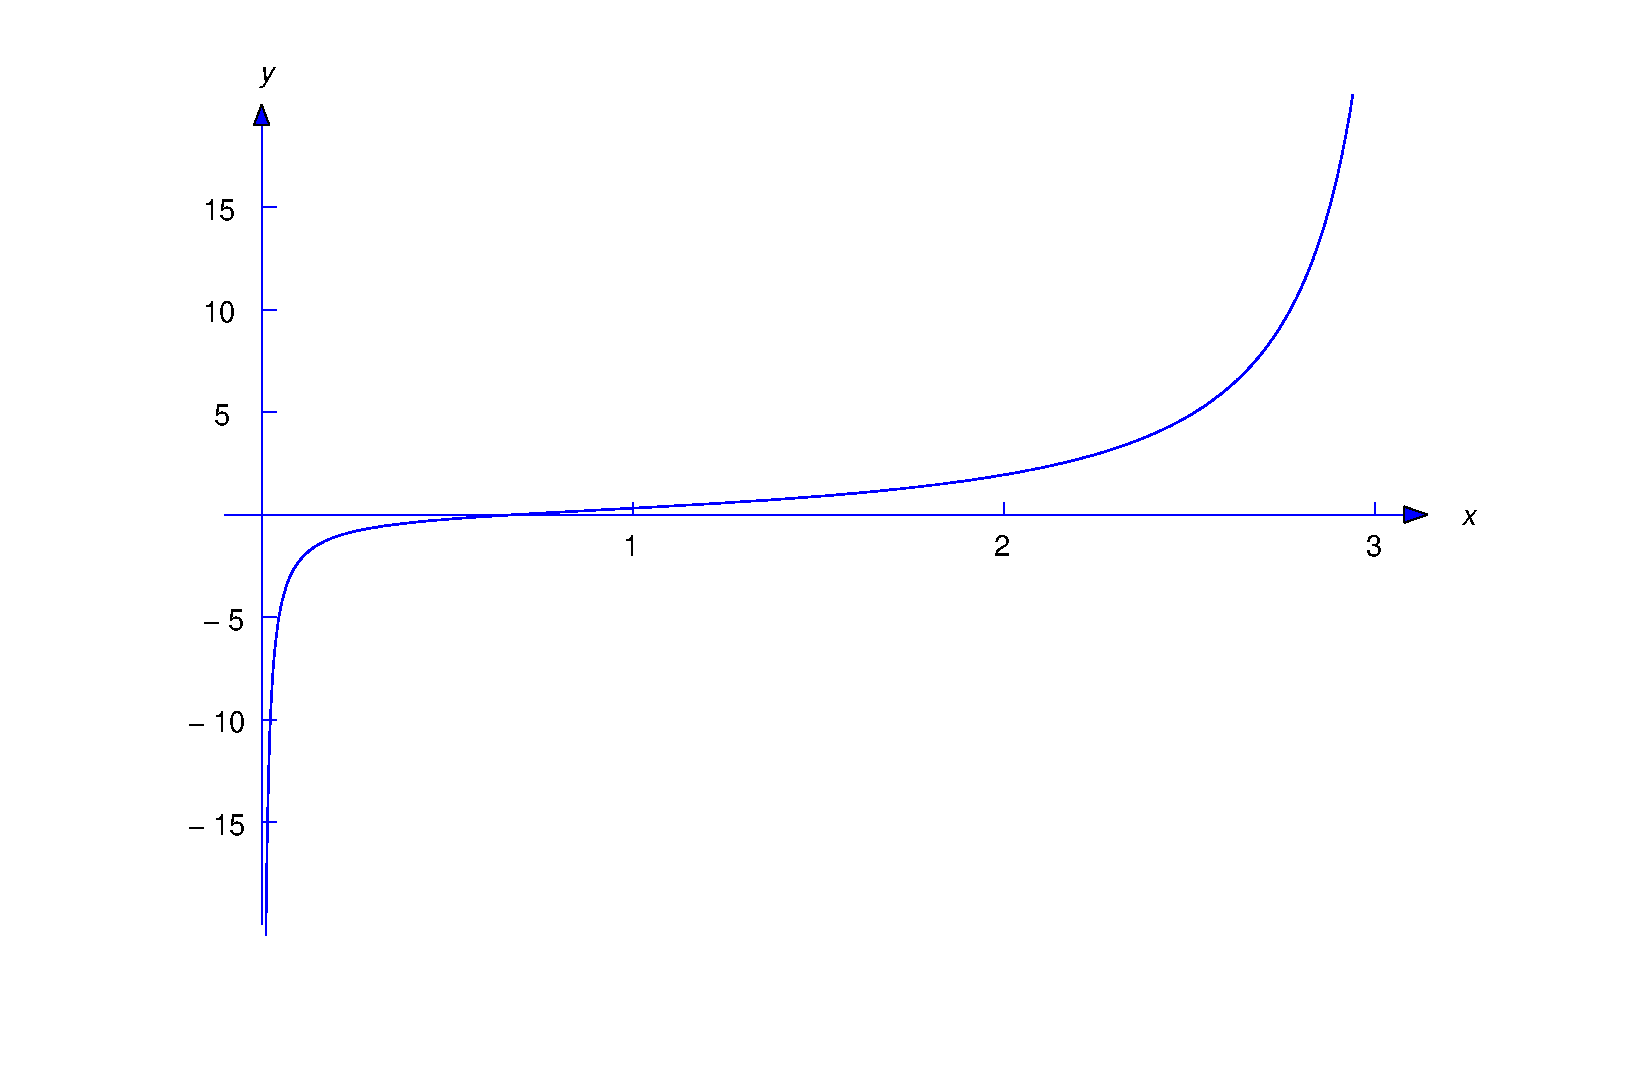
\includegraphics[bb=-78 148 689 643, width=5.67in, height=3.66in, keepaspectratio]{fig020104}}
  \color{blue}
  \caption{Solution of $y'+(\cot x)y=x\csc x$, $y(\pi/2)=1$}
  \label{figure:2.1.4}
\end{figure}

\color{blue}
\remark{It wasn't necessary to do the computations \eqref{eq:2.1.23} and \eqref{eq:2.1.24} in
Example~\ref{example:2.1.6}, since we showed in the discussion preceding Example~\ref{example:2.1.5}
that if $y=uy_{1}$ where $y_{1}'+p(x)y_{1}=0$, then $y'+p(x)y=u'y_{1}$. We did these computations so
you would see this happen in this specific example. We recommend that you include these
``unnecessary'' computations in doing exercises, until you're confident that you really understand
the method. After that, omit them.}
\color{black}
\end{examplesolution}

\medskip

We summarize the method of variation of parameters for solving

\begin{equation}
  \label{eq:2.1.26}y'+p(x)y=f(x)
\end{equation}
as follows:

\medskip
\color{blue}
\begin{alist}
  \item % (a)
  Find a function $y_{1}$ such that
  \[
    \frac{y_{1}'}{y_{1}}=-p(x).
  \]
  For convenience, take the constant of integration to be zero.

  \item % (b)
  Write
  \begin{equation}
    \label{eq:2.1.27}y=uy_{1}
  \end{equation}
  to remind yourself of what you're doing.

  \item % (c)
  Write $u'y_{1}=f$ and solve for $u'$; thus, $u'=f/y_{1}$.

  \item % (d
  Integrate $u'$ to obtain $u$, with an arbitrary constant of integration.

  \item % (e)
  Substitute $u$ into \eqref{eq:2.1.27} to obtain $y$.
\end{alist}
\color{black}

\medskip
To solve an equation written as
\[
  P_{0}(x)y'+P_{1}(x)y=F(x),
\]
we recommend that you divide through by $P_{0}(x)$ to obtain an equation of the form
\eqref{eq:2.1.26} and then follow this procedure.

\boxit{Solutions in Integral Form}

\noindent
Sometimes the integrals that arise in solving a linear first order equation can't be evaluated in
terms of elementary functions. In this case the solution must be left in terms of an integral.

\begin{example}
  \label{example:2.1.7}\rm \mbox{}
  \newline
  \begin{alist}
    \item % (a)
    Find the general solution of
    \[
      y'-2xy=1.
    \]

    \item % (b)
    Solve the initial value problem
    \begin{equation}
      \label{eq:2.1.28}y'-2xy=1,\quad y(0)=y_{0}.
    \end{equation}
  \end{alist}
\end{example}

\begin{examplesolution}
\solutionpart{a} To apply variation of parameters, we need a nontrivial solution $y_{1}$ of the
complementary equation; thus, $y_{1}'-2xy_{1}=0$, which we rewrite as
\[
  \frac{y_{1}'}{y_{1}}=2x.
\]
Integrating this and taking the constant of integration to be zero yields
\[
  \ln|y_{1}|=x^{2},\mbox{\quad so \quad}|y_{1}|=e^{x^{2}}.
\]
We choose $y_{1}=e^{x^{2}}$ and seek solutions of \eqref{eq:2.1.28} in the form $y=ue^{x^{2}}$,
where
\[
  u'e^{x^{2}}=1,\mbox{\quad so \quad}u'=e^{-x^{2}}.
\]
Therefore
\[
  u=c+\int e^{-x^{2}}dx,
\]
but we can't simplify the integral on the right because there's no elementary function with
derivative equal to $e^{-x^{2}}$. Therefore the best available form for the general solution of
\eqref{eq:2.1.28} is
\begin{equation}
  \label{eq:2.1.29}y=ue^{x^{2}}=e^{x^{2}}\left(c+\int e^{-x^{2}}dx\right).
\end{equation}

\solutionpart{b} Since the initial condition in \eqref{eq:2.1.28} is imposed at $x_{0}=0$, it is
convenient to rewrite \eqref{eq:2.1.29} as
\[
  y=e^{x^{2}}\left(c+\int^{x}_{0}e^{-t^{2}}dt\right),\mbox{\quad since \quad}\int_{0}^{0}e^{-t^{2}}\,dt=0.
\]
Setting $x=0$ and $y=y_{0}$ here shows that $c=y_{0}$. Therefore the solution of the initial value
problem is
\begin{equation}
  \label{eq:2.1.30}y=e^{x^{2}}\left(y_{0}+\int^{x}_{0}e^{-t^{2}}dt\right).
\end{equation}
For a given value of $y_{0}$ and each fixed $x$, the integral on the right can be evaluated by
numerical methods. An alternate procedure is to apply the numerical integration procedures discussed
in Chapter~3 directly to the initial value problem \eqref{eq:2.1.28}. Figure~\ref{figure:2.1.5}
shows graphs of \eqref{eq:2.1.30} for several values of $y_{0}$.

\begin{figure}[H]
  \centering
  \scalebox{.9}{
  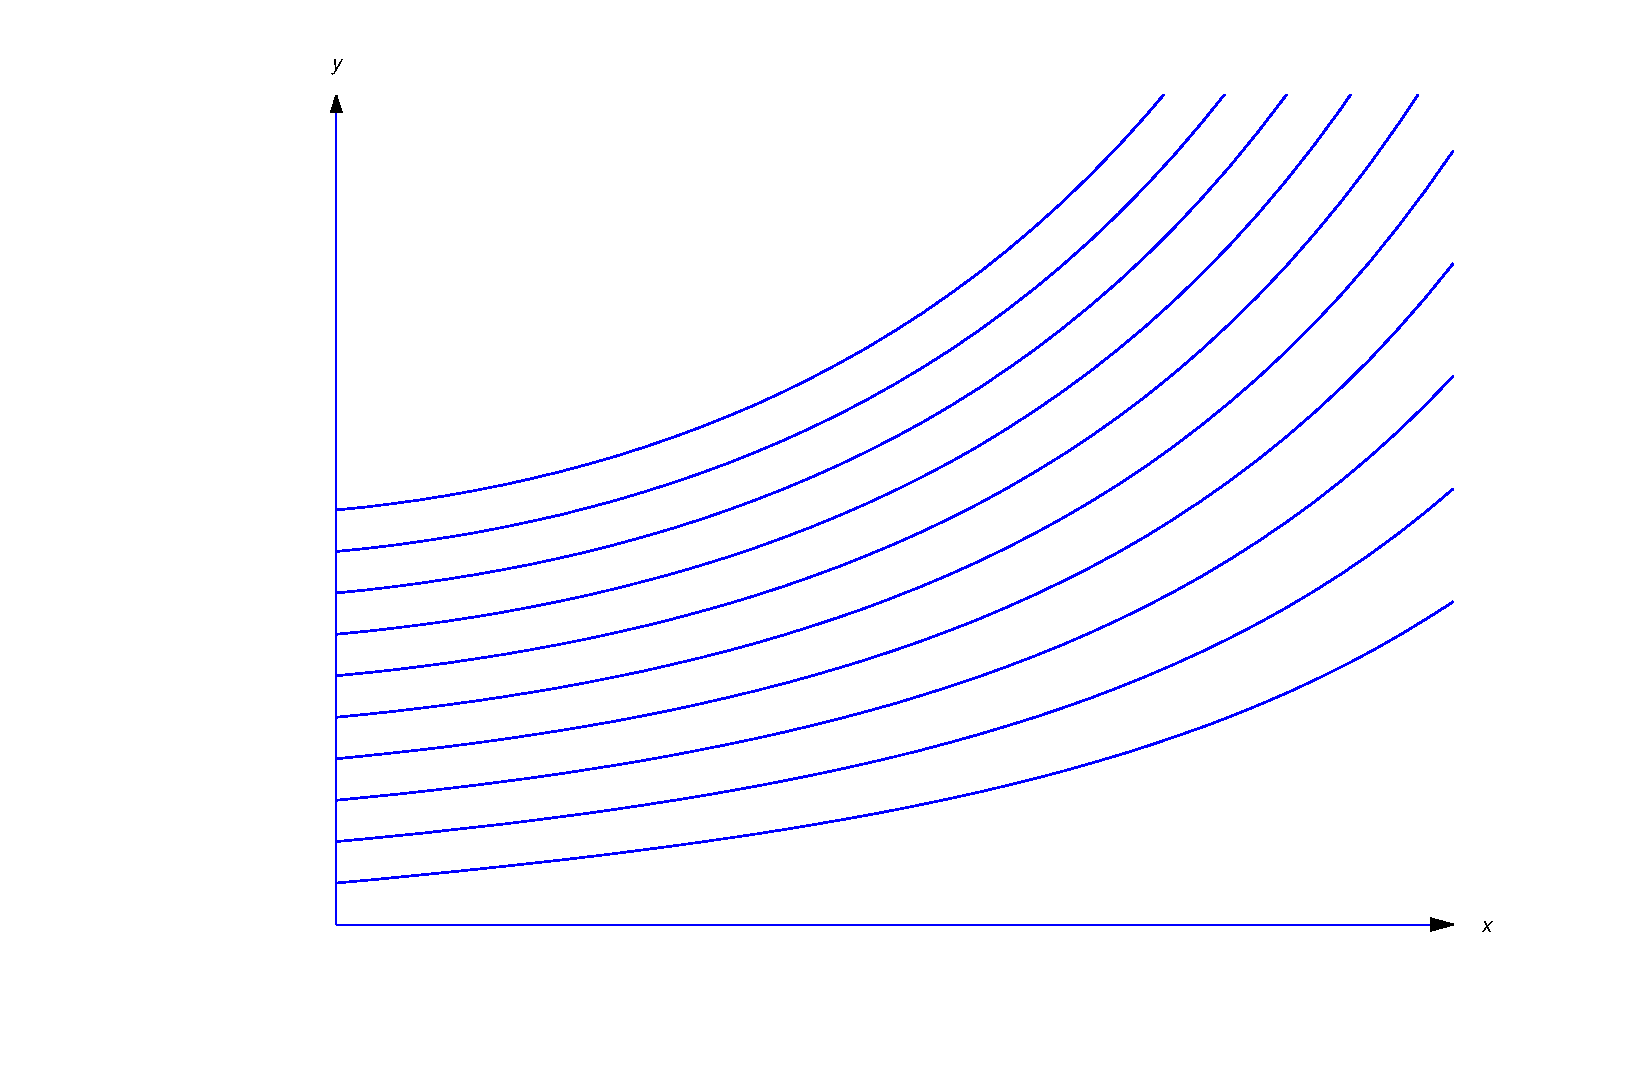
\includegraphics[bb=-78 148 689 643, width=5.67in, height=3.66in, keepaspectratio]{fig020105}
  }
  \color{blue}
  \caption{Solutions of $y'-2xy=1$, $y(0)=y_{0}$}
  \label{figure:2.1.5}
\end{figure}
\end{examplesolution}

\boxit{An Existence and Uniqueness Theorem}

\noindent
The method of variation of parameters leads to this theorem.

\begin{theorem}
  \color{blue}
  \label{thmtype:2.1.2} Suppose $p$ and $f$ are continuous on an open interval $(a,b)$, and let
  $y_{1}$ be any nontrivial solution of the complementary equation
  \[
    y'+p(x)y=0
  \]
  on $(a,b)$. Then:
  \begin{alist}
    \item % (a)
    The general solution of the nonhomogeneous equation
    \begin{equation}
      \label{eq:2.1.31}y'+p(x)y=f(x)
    \end{equation}
    on $(a,b)$ is
    \begin{equation}
      \label{eq:2.1.32}y=y_{1}(x)\left(c+\int f(x)/y_{1}(x)\,dx\right).
    \end{equation}

    \item % (b)
    If $x_{0}$ is an arbitrary point in $(a,b)$ and $y_{0}$ is an arbitrary real number, then the
    initial value problem
    \[
      y'+p(x)y=f(x),\quad y(x_{0})=y_{0}
    \]
    has the unique solution
    \[
      y=y_{1}(x)\left(\frac{y_{0}}{y_{1}(x_{0})}+\int^{x}_{x_{0}}\frac{f(t)}{y_{1}(t)}\,dt\right)
    \]
    on $(a,b)$.
  \end{alist}
\end{theorem}

\proof \part{a} To show that \eqref{eq:2.1.32} is the general solution of \eqref{eq:2.1.31} on
$(a,b)$, we must prove that:

\begin{rmlist}
  \item % (i)
  If $c$ is any constant, the function $y$ in \eqref{eq:2.1.32} is a solution of \eqref{eq:2.1.31}
  on $(a,b)$.

  \item % (ii)
  If $y$ is a solution of \eqref{eq:2.1.31} on $(a,b)$ then $y$ is of the form \eqref{eq:2.1.32} for
  some constant~$c$.
\end{rmlist}

To prove \part{i}, we first observe that any function of the form \eqref{eq:2.1.32} is defined on
$(a,b)$, since $p$ and $f$ are continuous on $(a,b)$. Differentiating \eqref{eq:2.1.32} yields
\[
  y'=y_{1}'(x)\left(c+\int f(x)/y_{1}(x)\, dx\right)+f(x).
\]
Since $y_{1}'=-p(x)y_{1}$, this and \eqref{eq:2.1.32} imply that
\begin{eqnarray*}
  y' & = & -p(x)y_{1}(x)\left(c+\int f(x)/y_{1}(x)\,dx\right)+f(x) \\
     & = & -p(x)y(x)+f(x),
\end{eqnarray*}
which implies that $y$ is a solution of \eqref{eq:2.1.31}.

To prove \part{ii}, suppose $y$ is a solution of \eqref{eq:2.1.31} on $(a,b)$. From the proof of
Theorem~\ref{thmtype:2.1.1}, we know that $y_{1}$ has no zeros on $(a,b)$, so the function
$u=y/y_{1}$ is defined on $(a,b)$. Moreover, since
\[
  y'=-py+f\mbox{\quad and\quad}y_{1}'=-py_{1},
\]
\begin{eqnarray*}
  u' & = & \frac{y_{1}y'-y_{1}'y}{y_{1}^{2}} \\[2\jot]
     & = & \frac{y_{1}(-py+f)-(-py_{1})y}{y_{1}^{2}}=\frac{f}{y_{1}}.
\end{eqnarray*}
Integrating $u'=f/y_{1}$ yields
\[
  u=\left(c+\int f(x)/y_{1}(x)\,dx\right),
\]
which implies \eqref{eq:2.1.32}, since $y=uy_{1}$.

\part{b} We've proved \part{a}, where $\int f(x)/y_{1}(x)\,dx$ in \eqref{eq:2.1.32} is an arbitrary
antiderivative of $f/y_{1}$. Now it's convenient to choose the antiderivative that equals zero when
$x=x_{0}$, and write the general solution of \eqref{eq:2.1.31} as
\[
  y=y_{1}(x)\left(c+\int^{x}_{x_{0}}\frac{f(t)}{y_{1}(t)}\,dt\right).
\]
Since
\[
  y(x_{0})=y_{1}(x_{0})\left(c+\int^{x_{0}}_{x_{0}}\frac{f(t)}{y_{1}(t)}\,dt\right)=cy_{1}(x_{0}),
\]
we see that $y(x_{0})=y_{0}$ if and only if $c=y_{0}/y_{1}(x_{0})$.

\exercises In Exercises~\ref{exer:2.1.1}--\ref{exer:2.1.5} find the general solution.

\begin{exerciselist}
  \begin{tabular}[t]{@{}p{168pt}@{}p{168pt}}
    \item\label{exer:2.1.1} $y'+ay=0$ ($a$=constant) &
    \item\label{exer:2.1.2}\vspace*{10pt} $y'+3x^{2}y=0$
  \end{tabular}

  \begin{tabular}[t]{@{}p{168pt}@{}p{168pt}}
    \item\label{exer:2.1.3} $xy'+(\ln x)y=0$ &
    \item\label{exer:2.1.4} $xy'+3y=0$
  \end{tabular}

  \begin{tabular}[t]{@{}p{168pt}@{}p{168pt}}
    \item\label{exer:2.1.5} $x^{2}y'+y=0$ &
  \end{tabular}

  \exercisetext{In Exercises~\ref{exer:2.1.6}--\ref{exer:2.1.11} solve the initial value problem.}

  \item\label{exer:2.1.6} $\dst{y'+\left(\frac{1+x}{x}\right)y=0,\quad y(1)=1}$

  \item\label{exer:2.1.7} $\dst{xy'+\left(1+\frac{1}{\ln x}\right)y=0,\quad y(e)=1}$

  \item\label{exer:2.1.8} $\dst{xy'+(1+x\cot x)y=0,\quad y\left(\frac{\pi}{2} \right)=2}$

  \item\label{exer:2.1.9} $\dst{y'-\left(\frac{2x}{1+x^{2}}\right)y=0,\quad y(0)=2}$

  \item\label{exer:2.1.10} $\dst{y'+\frac{k}{x}y=0,\quad y(1)=3 \quad\mbox{($k$= constant)}}$

  \item\label{exer:2.1.11} $\dst y'+(\tan kx)y=0,\quad y(0)=2 \quad\mbox{($k=$ constant)}$

  \exercisetext{In Exercises~\ref{exer:2.1.12} --\ref{exer:2.1.15} find the general solution. Also,
  plot a direction field and some integral curves on the rectangular region
  $\{-2\le x\le2,\ -2\le y\le2$\}.}

  \begin{tabular}{@{}p{168pt}@{}p{168pt}}
    \item\label{exer:2.1.12} \CGex $y'+3y=1$ &
    \item\label{exer:2.1.13}\vspace*{6pt} \CGex $\dst{y'+\left(\frac{1}{x}- 1\right)y=-\frac{2}{x}}$
  \end{tabular}

  \begin{tabular}{@{}p{168pt}@{}p{168pt}}
    \item\label{exer:2.1.14} \CGex $y'+2xy=xe^{-x^{2}}$ &
    \item\label{exer:2.1.15} \CGex $\dst{y'+\frac{2x}{1+x^{2}}y=\frac{e^{-x}}{1+x^{2}}}$
  \end{tabular}

  \exercisetext{In Exercises~\ref{exer:2.1.16} --\ref{exer:2.1.24} find the general solution.}

  \begin{tabular}[t]{@{}p{168pt}@{}p{168pt}}
    \item\label{exer:2.1.16} $\dst{y'+\frac{1}{x}y=\frac{7}{x^{2}}+3}$ &
    \item\label{exer:2.1.17}\vspace*{8pt} $\dst{y'+\frac{4}{x-1}y =\frac{1}{(x-1)^{5}}+\frac{\sin x}{(x-1)^{4}}}$
  \end{tabular}

  \begin{tabular}[t]{@{}p{168pt}@{}p{168pt}}
    \item\label{exer:2.1.18} $xy'+(1+2x^{2})y=x^{3}e^{-x^{2}}$ &
    \item\label{exer:2.1.19}\vspace*{-8pt} $\dst{xy'+2y=\frac{2}{x^{2}}+1}$
  \end{tabular}

  \begin{tabular}[t]{@{}p{168pt}@{}p{168pt}}
    \item\label{exer:2.1.20} $y'+(\tan x)y=\cos x$ &
    \item\label{exer:2.1.21}\vspace*{-5pt} $\dst{(1+x)y'+2y=\frac{\sin x}{1+x}}$
  \end{tabular}

  \item\label{exer:2.1.22} $(x-2)(x-1)y'-(4x-3)y=(x-2)^{3}$

  \begin{tabular}[t]{@{}p{168pt}@{}p{168pt}}
    \item\label{exer:2.1.23} $y'+(2\sin x\cos x)y=e^{-\sin^{2}x}$ &
    \item\label{exer:2.1.24} $x^{2}y'+3xy=e^{x}$
  \end{tabular}

  \exercisetext{In Exercises~\ref{exer:2.1.25}--\ref{exer:2.1.29} solve the initial value problem
  and sketch the graph of the solution.}

  \item\label{exer:2.1.25} \CGex $y'+7y=e^{3x},\quad y(0)=0$

  \item\label{exer:2.1.26} \CGex $\dst{(1+x^{2})y'+4xy=\frac{2}{1+x^{2}},\quad y(0)=1}$

  \item\label{exer:2.1.27} \CGex $\dst{xy'+3y=\frac{2}{x(1+x^{2})},\quad y(-1)=0}$

  \item\label{exer:2.1.28} \CGex $\dst{y'+(\cot x)y=\cos x,\quad y\left(\frac{\pi}{2}\right)=1}$

  \item\label{exer:2.1.29} \CGex $\dst{y'+\frac{1}{x}y=\frac{2}{x^{2}}+1,\quad y(-1)=0}$

  \exercisetext{In Exercises~\ref{exer:2.1.30}--\ref{exer:2.1.37} solve the initial value problem.}

  \item\label{exer:2.1.30}
        $\dst{(x-1)y'+3y=\frac{1}{(x-1)^{3}}+ \frac{\sin x}{(x-1)^{2}},\quad y(0)=1}$

  \item\label{exer:2.1.31} $xy'+2y=8x^{2},\quad y(1)=3$

  \item\label{exer:2.1.32} $xy'-2y=-x^{2},\quad y(1)=1$

  \item\label{exer:2.1.33} $y'+2xy=x,\quad y(0)=3$

  \item\label{exer:2.1.34} $\dst{(x-1)y'+3y=\frac{1+(x-1)\sec^{2}x}{(x-1)^{3}},\quad y(0)=-1}$

  \item\label{exer:2.1.35} $\dst{(x+2)y'+4y=\frac{1+2x^{2}}{x(x+2)^{3}},\quad y(-1)=2}$

  \item\label{exer:2.1.36} $(x^{2}-1)y'-2xy=x(x^{2}-1),\quad y(0)=4$

  \item\label{exer:2.1.37} $(x^{2}-5)y'-2xy=-2x(x^{2}-5),\quad y(2)=7$

  \exercisetext{In Exercises~\ref{exer:2.1.38}--\ref{exer:2.1.42} solve the initial value problem
  and leave the answer in a form involving a definite integral. (You can solve these problems
  numerically by methods discussed in Chapter~3.)}

  \item\label{exer:2.1.38} $y'+2xy=x^{2},\quad y(0)=3$

  \item\label{exer:2.1.39} $\dst{y'+\frac{1}{x}y=\frac{\sin x}{x^{2}},\quad y(1)=2}$

  \item\label{exer:2.1.40} $\dst{y'+y=\frac{e^{-x}\tan x}{x},\quad y(1)=0}$

  \item\label{exer:2.1.41} $\dst{y'+\frac{2x}{1+x^{2}}y=\frac{e^{x}}{(1+x^{2})^{2}},\quad y(0)=1}$

  \item\label{exer:2.1.42} $xy'+(x+1)y=e^{x^{2}},\quad y(1)=2$

  \item\label{exer:2.1.43}

  Experiments indicate that glucose is absorbed by the body at a rate proportional to the amount of
  glucose present in the bloodstream. Let $\lambda$ denote the (positive) constant of
  proportionality. Now suppose glucose is injected into a patient's bloodstream at a constant rate
  of $r$ units per unit of time. Let $G=G(t)$ be the number of units in the patient's bloodstream at
  time $t>0$. Then
  \[
    G'=-\lambda G+r,
  \]
  where the first term on the right is due to the absorption of the glucose by the patient's body
  and the second term is due to the injection. Determine $G$ for $t>0$, given that $G(0)=G_{0}$.
  Also, find $\lim_{t\to\infty}G(t)$.

  \item\label{exer:2.1.44}
  \begin{alist}
    \item % (a)
    \Lex Plot a direction field and some integral curves for
    \[
      xy'-2y=-1 \eqno{\rm(A)}
    \]
    on the rectangular region $\{-1\le x\le1,-.5\le y\le1.5\}$. What do all the integral curves have
    in common?

    \item % (b)
    Show that the general solution of (A) on $(-\infty,0)$ and $(0,\infty)$ is
    \[
      y=\frac{1}{2}+cx^{2}.
    \]

    \item % (c)
    Show that $y$ is a solution of (A) on $(-\infty,\infty)$ if and only if
    \[
      y=\left\{
      \begin{array}{ll}
        \dst{\frac{1}{2}+c_{1}x^{2}}, & x \ge0, \\[2\jot]
        \dst{\frac{1}{2}+c_{2}x^{2}}, & x<0,
      \end{array}\right.
    \]
    where $c_{1}$ and $c_{2}$ are arbitrary constants.

    \item % (c)
    Conclude from \part{c} that all solutions of (A) on $(-\infty,\infty)$ are solutions of the
    initial value problem
    \[
      xy'-2y=-1,\quad y(0)=\frac{1}{2}.
    \]

    \item % (d)
    Use \part{b} to show that if $x_{0}\ne0$ and $y_{0}$ is arbitrary, then the initial value
    problem
    \[
      xy'-2y=-1,\quad y(x_{0})=y_{0}
    \]
    has infinitely many solutions on ($-\infty,\infty$). Explain why this doesn't contradict
    Theorem~\ref{thmtype:2.1.2}\part{b}.
  \end{alist}

  \item\label{exer:2.1.45} Suppose $f$ is continuous on an open interval $(a,b)$ and $\alpha$ is a
        constant.
  \begin{alist}
    \item % (a)
    Derive a formula for the solution of the initial value problem
    \renewcommand{\theequation}{\Alph{equation}}
    \[
      y'+\alpha y=f(x),\quad y(x_{0})=y_{0}, \eqno{\rm(A)}
    \]
    where $x_{0}$ is in $(a,b)$ and $y_{0}$ is an arbitrary real number.

    \item % (b)
    Suppose $(a,b)=(a,\infty)$, $\alpha>0$ and $\displaystyle{\lim_{x\to\infty}f(x)=L}$. Show that
    if $y$ is the solution of (A), then $\displaystyle{\lim_{x\to \infty}y(x)=L/\alpha}$.
  \end{alist}

  \item\label{exer:2.1.46} Assume that all functions in this exercise are defined on a common
        interval $(a,b)$.
  \begin{alist}
    \item % (a)
    Prove: If $y_{1}$ and $y_{2}$ are solutions of
    \[
      y'+p(x)y=f_{1}(x)
    \]
    and
    \[
      y'+p(x)y=f_{2}(x)
    \]
    respectively, and $c_{1}$ and $c_{2}$ are constants, then $y=c_{1}y_{1}+c_{2}y_{2}$ is a
    solution of
    \[
      y'+p(x)y=c_{1}f_{1}(x)+c_{2}f_{2}(x).
    \]
    (This is the {\it principle of superposition.\/})

    \item % (b)
    Use \part{a} to show that if $y_{1}$ and $y_{2}$ are solutions of the nonhomogeneous equation
    \[
      y'+p(x)y=f(x), \eqno{\rm(A)}
    \]
    then $y_{1}-y_{2}$ is a solution of the homogeneous equation
    \[
      y'+p(x)y=0. \eqno{\rm(B)}
    \]

    \item % (c)
    Use \part{a} to show that if $y_{1}$ is a solution of (A) and $y_{2}$ is a solution of (B), then
    $y_{1}+y_{2}$ is a solution of (A).
  \end{alist}

  \item\label{exer:2.1.47} Some nonlinear equations can be transformed into linear equations by
        changing the dependent variable. Show that if
  \[
    g'(y)y'+p(x)g(y)=f(x)
  \]
  where $y$ is a function of $x$ and $g$ is a function of $y$, then the new dependent variable
  $z=g(y)$ satisfies the linear equation
  \[
    z'+p(x)z=f(x).
  \]

  \item\label{exer:2.1.48} Solve by the method discussed in Exercise~\ref{exer:2.1.47}.

  \vspace*{6pt}
  \begin{tabular}[t]{@{}p{168pt}@{}p{168pt}}
    {\bf (a)} $(\sec^{2}y)y'-3\tan y=-1$ & {\bf (b)} $\dst{e^{y^{2}}\left(2yy'+ \frac{2}{x}\right)=\frac{1}{x^{2}}}$
  \end{tabular}

  \begin{tabular}[t]{@{}p{168pt}@{}p{168pt}}
    {\bf (c)} $\dst{\frac{xy'}{y}+2\ln y=4x^{2}}$ & {\bf (d)} $\dst{\frac{y'}{(1+y)^{2}}- \frac{1}{x(1+y)}=-\frac{3}{x^{2}}}$
  \end{tabular}

  \item\label{exer:2.1.49} We've shown that if $p$ and $f$ are continuous on $(a,b)$ then every
        solution of
  \[
    y'+p(x)y=f(x) \eqno{\rm(A)}
  \]
  on $(a,b)$ can be written as $y=uy_{1}$, where $y_{1}$ is a nontrivial solution of the
  complementary equation for (A) and $u'=f/y_{1}$. Now suppose $f$, $f'$, \dots, $f^{(m)}$ and $p$,
  $p'$, \dots, $p^{(m-1)}$ are continuous on $(a,b)$, where $m$ is a positive integer, and define
  \begin{eqnarray*}
    f_{0} & = & f, \\
    f_{j} & = & f_{j-1}'+pf_{j-1},\quad1\le j\le m.
  \end{eqnarray*}
  Show that
  \[
    u^{(j+1)}=\frac{f_{j}}{y_{1}},\quad0\le j\le m.
  \]
\end{exerciselist}


\section{Separable Equations}

\noindent
A first order differential equation  is  {\color{blue}\it
separable} if it can be written as
\begin{equation} \label{eq:2.2.1}
h(y)y'=g(x),
\end{equation}
where the left side is a product of $y'$ and a function of $y$ and
the right side is a function of $x$. Rewriting a separable
differential equation in this form is called {\color{blue}\it separation of
variables.\/} In Section~2.1 we used separation of variables
to solve homogeneous linear equations. In this section we'll apply
this method to nonlinear equations.

To see how to solve \eqref{eq:2.2.1}, let's first assume that $y$
is a solution.
Let  $G(x)$ and $H(y)$ be antiderivatives of $g(x)$
and $h(y)$; that is,
\begin{equation} \label{eq:2.2.2}
H'(y)=h(y)\mbox{\quad and \quad}G'(x)=g(x).
\end{equation}
Then, from the chain rule,
$$
\frac{d}{dx}H(y(x))=H'(y(x))y'(x)=h(y)y'(x).
$$
Therefore \eqref{eq:2.2.1} is equivalent to
$$
\frac{d}{dx}H(y(x))=\frac{d}{dx}G(x).
$$
Integrating both sides of this equation and combining the constants of
integration yields
\begin{equation} \label{eq:2.2.3}
H(y(x))=G(x)+c.
\end{equation}
Although we derived this equation on the assumption that $y$
is a solution of \eqref{eq:2.2.1}, we can now view it differently:
Any differentiable function $y$ that satisfies \eqref{eq:2.2.3}
for some constant $c$ is a solution of \eqref{eq:2.2.1}. To see this, we
differentiate both sides of \eqref{eq:2.2.3}, using the chain rule on the
left, to obtain
$$
H'(y(x))y'(x)=G'(x),
$$
which is equivalent to
$$
h(y(x))y'(x)=g(x)
$$
because of \eqref{eq:2.2.2}.

In conclusion, to solve \eqref{eq:2.2.1} it suffices to find
functions $G=G(x)$ and $H=H(y)$ that satisfy \eqref{eq:2.2.2}.
Then any differentiable function  $y=y(x)$  that satisfies
\eqref{eq:2.2.3} is a solution of \eqref{eq:2.2.1}.

\begin{example}\label{example:2.2.1}\rm
Solve the equation
$$
y'=x(1+y^{2}).
$$
\end{example}

\solution Separating variables
yields
$$
\frac{y'}{1+y^{2}}=x.
$$
Integrating yields
$$
\tan^{-1}y=\frac{x^{2}}{2}+c
$$
Therefore
$$
y=\tan\left(\frac{x^{2}}{2}+c\right).
$$

\begin{example}\label{example:2.2.2} \rm  \mbox{}\newline
\begin{alist}
\item %(a)
Solve the equation
\begin{equation} \label{eq:2.2.4}
y'=-\frac{x}{y}.
\end{equation}

\item %(b)
Solve the initial value problem
\begin{equation} \label{eq:2.2.5}
y'=-\frac{x}{y},\quad y(1)=1.
\end{equation}

\item %(c)
Solve the initial value problem
\begin{equation} \label{eq:2.2.6}
y'=-\frac{x}{y},\quad y(1)=-2.
\end{equation}
\end{alist}
\end{example}

\solutionpart{a} Separating variables
in \eqref{eq:2.2.4}  yields
$$
yy'=-x.
$$
Integrating yields
$$
\frac{y^{2}}{2}=-\frac{x^{2}}{2}+c,\mbox{\quad or,\, equivalently, \quad}
x^{2}+y^{2}=2c.
$$
The last equation shows that $c$ must be positive if $y$ is to be a
solution of \eqref{eq:2.2.4} on an open interval. Therefore we let
$2c=a^{2}$ (with $a>0$) and rewrite the last equation as
\begin{equation} \label{eq:2.2.7}
x^{2}+y^{2}=a^{2}.
\end{equation}
 This equation has two differentiable solutions for $y$ in terms of
$x$:
\begin{equation} \label{eq:2.2.8}
y=\phantom{-}\sqrt{a^{2}-x^{2}},\quad-a<x<a,
\end{equation}
 and
\begin{equation} \label{eq:2.2.9}
y=-\sqrt{a^{2}-x^{2}},\quad-a<x<a.
\end{equation}
The solution curves defined by \eqref{eq:2.2.8}  are semicircles
above the
$x$-axis and  those defined by \eqref{eq:2.2.9}  are semicircles below the
$x$-axis (Figure~\ref{figure:2.2.1}).

\solutionpart{b}  The solution of  \eqref{eq:2.2.5}
is positive when $x=1$; hence, it  is of the form \eqref{eq:2.2.8}.
 Substituting $x=1$ and $y=1$ into \eqref{eq:2.2.7} to satisfy the
initial condition yields $a^{2}=2$; hence, the solution of
\eqref{eq:2.2.5}
is
$$
y=\sqrt{2-x^{2}},\quad-\sqrt{2}<x<\sqrt{2}.
$$

\solutionpart{c}  The solution of  \eqref{eq:2.2.6}
is negative when $x=1$ and   is therefore of the form \eqref{eq:2.2.9}.
 Substituting $x=1$ and $y=-2$ into \eqref{eq:2.2.7} to satisfy the
initial condition yields $a^{2}=5$. Hence, the solution of \eqref{eq:2.2.6}
is
$$
y=-\sqrt{5-x^{2}},\quad-\sqrt{5}<x<\sqrt{5}.
$$

\begin{figure}[H]
  \centering
  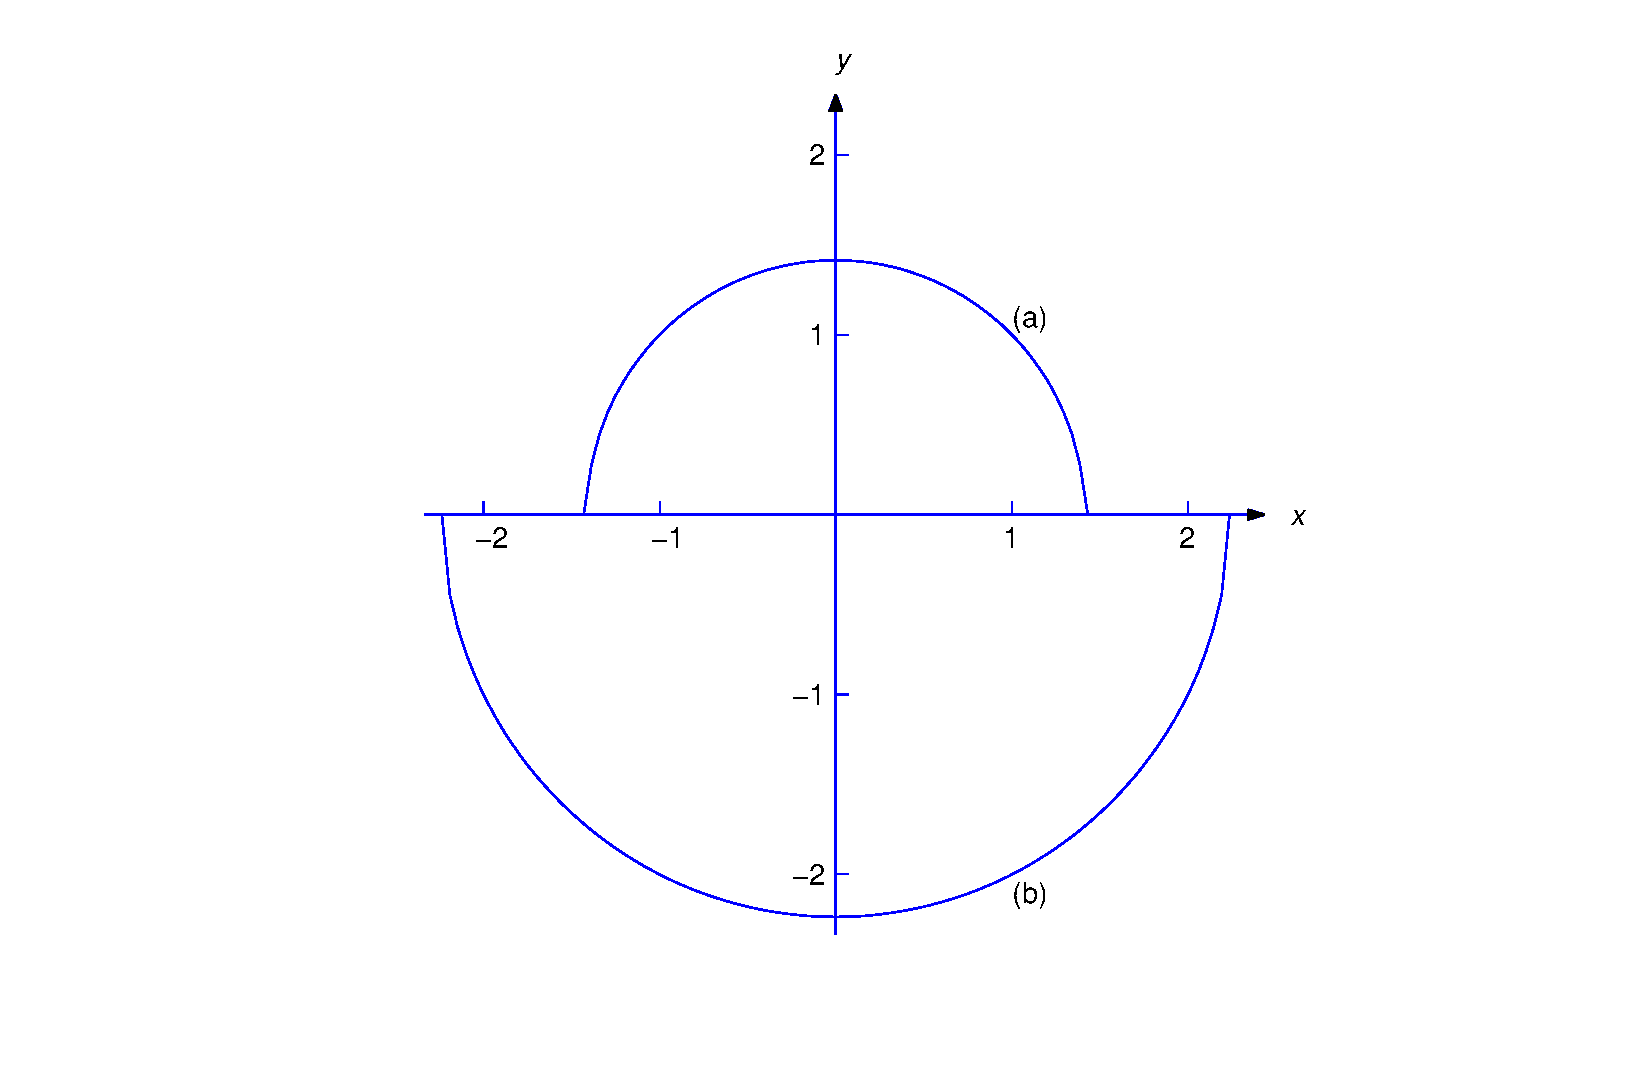
\includegraphics[bb=-78 148 689 643,width=5.67in,height=3.66in,keepaspectratio]{fig020201}
\color{blue}
  \caption{
{\bf (a)} $y=\sqrt{2-x^{2}}$,\, $-\sqrt{2}<x<\sqrt{2}$; \,
{\bf (b)} $y=-\sqrt{5-x^{2}}$,\, $-\sqrt{5}<x<\sqrt{5}$}
  \label{figure:2.2.1}
\end{figure}

\boxit{Implicit Solutions of Separable Equations}

\noindent
In Examples~\ref{example:2.2.1} and \ref{example:2.2.2} we were able to
solve the equation $H(y)=G(x)+c$ to obtain explicit formulas for
solutions of the given separable differential equations. As we'll
see in the next example, this isn't  always possible.
In this situation we must broaden our definition of a solution of a
separable equation. The next theorem provides the basis for this
modification.  We omit the proof, which requires a result from
advanced calculus called as the {\color{blue}\it implicit function
theorem\/}.

\begin{theorem}\color{blue}~\label{thmtype:2.2.1}
Suppose $g=g(x)$ is continuous on $(a,b)$ and $h=h(y)$
are continuous on $(c,d)$. Let $G$ be an antiderivative of
$g$ on $(a,b)$ and let $H$ be an antiderivative of $h$ on $(c,d)$.
Let $x_{0}$ be an arbitrary point in $(a,b)$, let $y_{0}$
be a point in $(c,d)$ such that $h(y_{0})\ne0$, and define
\begin{equation} \label{eq:2.2.10}
c=H(y_{0})-G(x_{0}).
\end{equation}
Then there's a function $y=y(x)$ defined on some open interval
$(a_{1},b_{1})$, where $a\le a_{1}<x_{0}<b_{1}\le b$, such that  $y(x_{0})=y_{0}$
and
\begin{equation} \label{eq:2.2.11}
H(y)=G(x)+c
\end{equation}
for $a_{1}<x<b_{1}$.
Therefore $y$ is a solution of the initial value problem
\begin{equation} \label{eq:2.2.12}
h(y)y'=g(x),\quad y(x_{0})=x_{0}.
\end{equation}
\end{theorem}

It's convenient to say that \eqref{eq:2.2.11} with $c$ arbitrary is an
{\color{blue}\it implicit solution\/} of $h(y)y'=g(x)$. Curves defined by
\eqref{eq:2.2.11} are integral curves of $h(y)y'=g(x)$. If $c$ satisfies
\eqref{eq:2.2.10}, we'll say that \eqref{eq:2.2.11} is an {\color{blue}\it
implicit
solution of the initial value problem\/} \eqref{eq:2.2.12}. However, keep
these  points in mind:
\begin{itemize}
\item  For some choices of $c$ there may not be any differentiable
functions $y$ that satisfy \eqref{eq:2.2.11}.
\item  The function $y$ in \eqref{eq:2.2.11} (not \eqref{eq:2.2.11} itself)
is a solution of $h(y)y'=g(x)$.
\end{itemize}

\begin{example}\label{example:2.2.3} \rm \mbox{}\newline
\begin{alist}
\item % (a)
Find implicit solutions of
\begin{equation} \label{eq:2.2.13}
y'=\frac{2x+1}{5y^{4}+1}.
\end{equation}
\item % (b)
Find an implicit solution of
\begin{equation} \label{eq:2.2.14}
y'=\frac{2x+1}{5y^{4}+1},\quad y(2)=1.
\end{equation}
\end{alist}
\end{example}

\solutionpart{a}
 Separating variables yields
$$
(5y^{4}+1)y'=2x+1.
$$
Integrating yields the implicit solution
\begin{equation} \label{eq:2.2.15}
y^{5}+y=x^{2}+x+c.
\end{equation}
of \eqref{eq:2.2.13}.

\solutionpart{b} Imposing the initial condition $y(2)=1$ in
\eqref{eq:2.2.15} yields $1+1=4+2+c$, so $c=-4$. Therefore
$$
y^{5}+y=x^{2}+x-4
$$
is an implicit solution of the initial value problem \eqref{eq:2.2.14}.
Although more than one differentiable function $y=y(x)$ satisfies
\ref{eq:2.2.13}) near $x=1$, it can be shown that there's only
one such function that satisfies the initial condition $y(1)=2$.

Figure~\ref{figure:2.2.2} shows a direction field and some integral curves
for \eqref{eq:2.2.13}.

\begin{figure}[tbp]
  \centering
  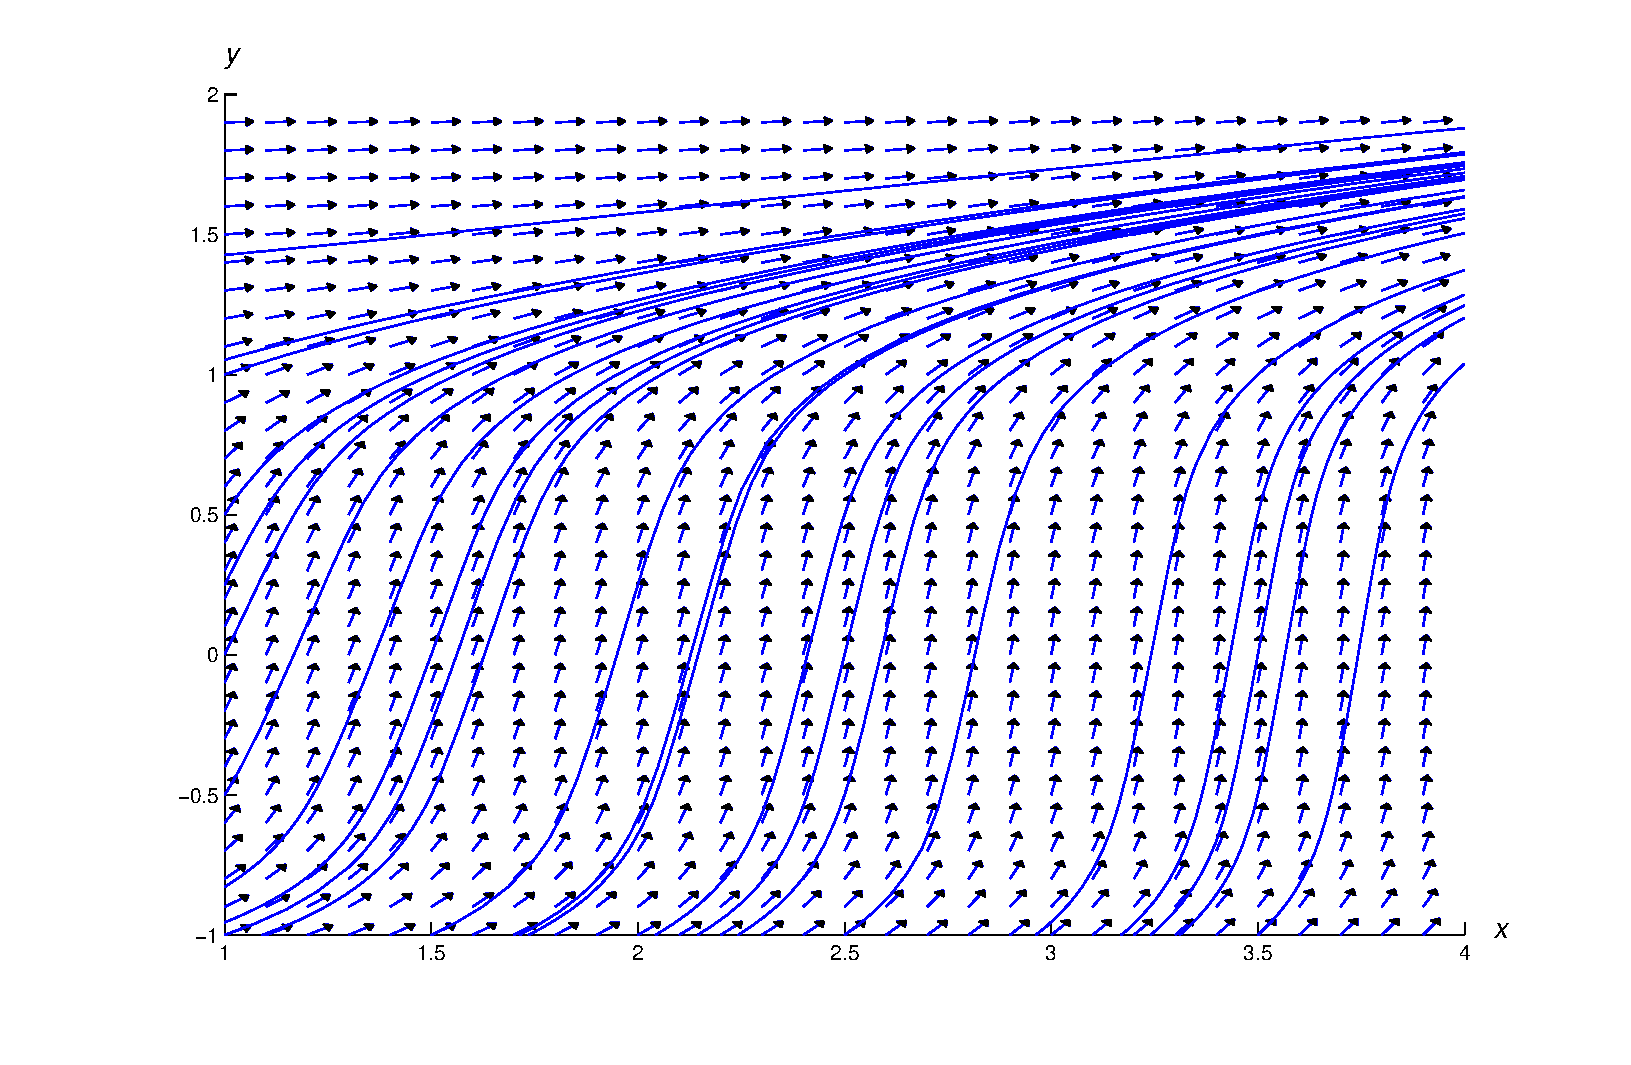
\includegraphics[bb=-78 148 689 643,width=5.67in,height=3.66in,keepaspectratio]{fig020202}
\color{blue}
  \caption{A direction field and integral curves for
$y'=\dst{\frac{2x+1}{5y^{4}+1}}$}
  \label{figure:2.2.2}
\end{figure}

\boxit{Constant Solutions of Separable Equations}

\noindent
An equation of the form
$$
y'=g(x)p(y)
$$
 is separable, since it can be rewritten as
$$
\frac{1}{p(y)}y'=g(x).
$$
 However, the division by  $p(y)$
is not legitimate  if $p(y)=0$ for some values of $y$.  The
next two examples show how to deal with this problem.

\begin{example}\label{example:2.2.4}
\rm  Find all solutions of
\begin{equation} \label{eq:2.2.16}
y'=2xy^{2}.
\end{equation}
\end{example}
\solution Here we must divide by $p(y)=y^{2}$ to separate variables.
This isn't  legitimate if $y$ is a solution of \eqref{eq:2.2.16} that
equals zero for some value of $x$. One such solution can be found by
inspection:  $y\equiv0$. Now suppose   $y$ is a solution
of \eqref{eq:2.2.16} that isn't  identically zero. Since $y$ is continuous
there must be an interval on which $y$ is never zero. Since division
by $y^{2}$ is legitimate for $x$ in this interval, we can separate
variables in \eqref{eq:2.2.16} to obtain
$$
\frac{y'}{y^{2}}=2x.
$$
 Integrating this yields
$$
-\frac{1}{y}=x^{2}+c,
$$
which is equivalent to
\begin{equation} \label{eq:2.2.17}
y=-\frac{1}{x^{2}+c}.
\end{equation}

We've now shown that if $y$ is a solution of \eqref{eq:2.2.16} that is
not identically zero, then $y$ must be of the form \eqref{eq:2.2.17}. By
substituting \eqref{eq:2.2.17} into \eqref{eq:2.2.16}, you can verify that
\eqref{eq:2.2.17} is  a solution of \eqref{eq:2.2.16}. Thus,
 solutions of \eqref{eq:2.2.16} are $y\equiv0$ and the functions
of the form \eqref{eq:2.2.17}. Note that the solution $y\equiv0$ isn't  of
the form \eqref{eq:2.2.17} for any value of $c$.

Figure~\ref{figure:2.2.3} shows a direction field and some integral
curves for \eqref{eq:2.2.16}

\begin{figure}[tbp]
  \centering
  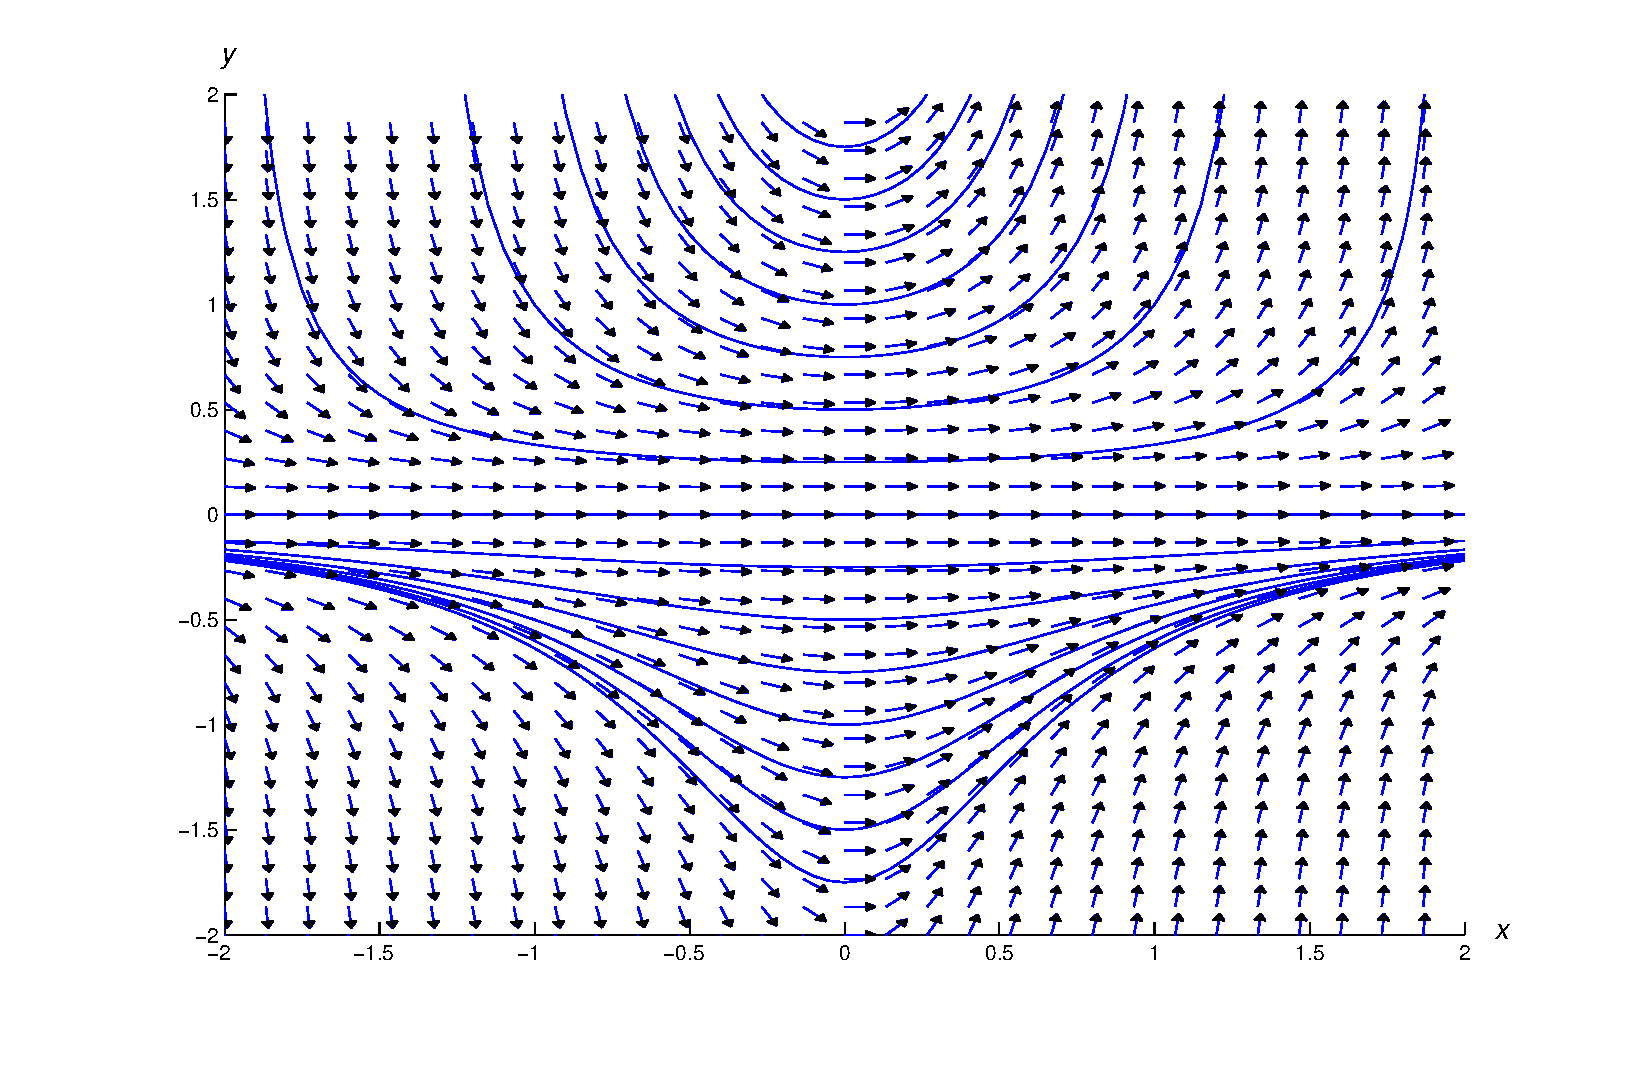
\includegraphics[bb=-78 148 689 643,width=5.67in,height=3.66in,keepaspectratio]{fig020203}
\color{blue}
  \caption{A direction field and  integral curves for $y'=2xy^{2}$}
  \label{figure:2.2.3}
\end{figure}

\begin{example}\label{example:2.2.5}
\rm  Find all solutions of
\begin{equation} \label{eq:2.2.18}
y'=\frac{1}{2}x(1-y^{2}).
\end{equation}
\end{example}

\solution Here we must divide by $p(y)=1-y^{2}$ to separate variables.
This isn't  legitimate if $y$ is a solution of \eqref{eq:2.2.18} that
equals $\pm1$ for some value of $x$. Two such solutions can be found
by inspection: $y\equiv1$ and $y\equiv-1$. Now suppose
$y$ is a solution of \eqref{eq:2.2.18} such that $1-y^{2}$ isn't
identically zero. Since $1-y^{2}$ is continuous there must be an
interval on which $1-y^{2}$ is never zero. Since division by $1-y^{2}$ is
legitimate for $x$ in this interval, we can separate variables in
\eqref{eq:2.2.18} to obtain
$$
\frac{2y'}{y^{2}-1}=-x.
$$
 A partial fraction expansion on the left yields
$$
\left[\frac{1}{y-1}-\frac{1}{y+1}\right]y'=-x,
$$
and integrating  yields
$$
\ln\left|\frac{y-1}{y+1}\right|=-\frac{x^{2}}{2}+k;
$$
 hence,
$$
\left|\frac{y-1}{y+1}\right|=e^{k}e^{-x^{2}/2}.
$$
 Since $y(x)\ne\pm1$ for $x$ on the interval under discussion, the
quantity
$(y-1)/(y+1)$  can't  change sign in this interval. Therefore
we can rewrite the last equation as
$$
\frac{y-1}{y+1}=ce^{-x^{2}/2},
$$
  where $c=\pm e^{k}$, depending upon the sign of $(y-1)/(y+1)$ on the
interval.
 Solving for  $y$ yields
\begin{equation} \label{eq:2.2.19}
y=\frac{1+ce^{-x^{2}/2}}{1-ce^{-x^{2}/2}}.
\end{equation}

We've now shown that if $y$ is a solution of \eqref{eq:2.2.18} that  is
not identically equal to $\pm1$, then $y$ must be as in
\eqref{eq:2.2.19}. By substituting \eqref{eq:2.2.19} into \eqref{eq:2.2.18} you
 can verify that \eqref{eq:2.2.19} is  a solution of
\eqref{eq:2.2.18}. Thus,  the solutions of \eqref{eq:2.2.18}
are $y\equiv1$, $y\equiv-1$ and the functions of the form
\eqref{eq:2.2.19}. Note that the constant solution $y\equiv1$ can be
obtained from this formula by taking $c=0$;     however, the other
constant solution, $y\equiv-1$, can't be obtained in this way.

Figure~\ref{figure:2.2.4} shows a direction field and some integrals for
\eqref{eq:2.2.18}.

\begin{figure}[H]
  \centering
  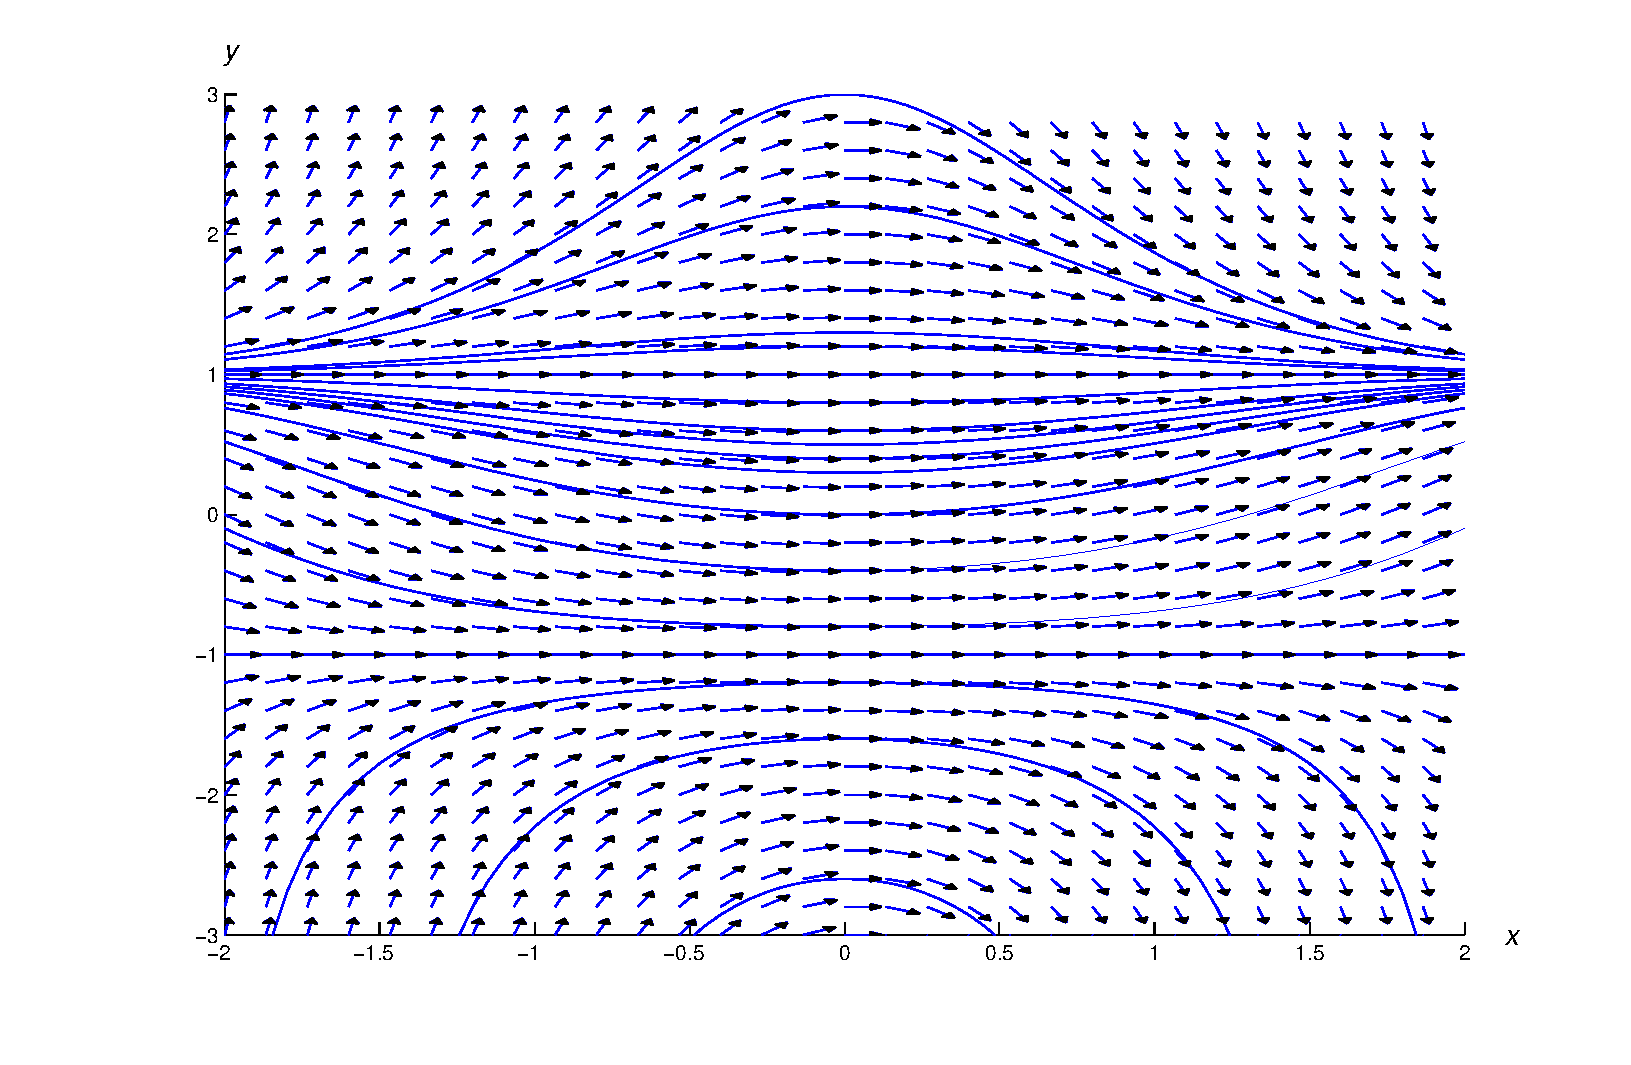
\includegraphics[bb=-78 148 689 643,width=5.67in,height=3.66in,keepaspectratio]{fig020204}
\color{blue}
\caption{
A direction field and integral curves for
$y'=\dst{\frac{x(1-y^{2})}{2}}$}
  \label{figure:2.2.4}
\end{figure}

\boxit{Differences Between Linear and Nonlinear Equations}

\noindent
Theorem~\ref{thmtype:2.1.2} states that if $p$ and $f$ are continuous on
$(a,b)$ then every solution of
$$
y'+p(x)y=f(x)
$$
 on  $(a,b)$  can be obtained by choosing a value for the constant
$c$  in the general solution, and   if
$x_{0}$ is any point in  $(a,b)$ and $y_{0}$ is arbitrary, then the
initial value problem
$$
y'+p(x)y=f(x),\quad y(x_{0})=y_{0}
$$
 has a solution on  $(a,b)$.

The not true for nonlinear equations. First, we
saw in Examples~\ref{example:2.2.4} and \ref{example:2.2.5} that a
nonlinear
equation may have solutions that can't be obtained by choosing a
specific value of a constant appearing in a one-parameter family of
solutions. Second, it is in general impossible to determine the
interval of validity of a solution to an initial value problem for a
nonlinear equation by simply examining the equation, since the
interval of validity may depend on the initial condition. For
instance, in Example~\ref{example:2.2.2} we saw that the solution of
$$
\frac{dy}{dx}=-\frac{x}{y},\quad y(x_{0})=y_{0}
$$
is valid on $(-a,a)$, where $a=\sqrt{x_{0}^{2}+y_{0}^{2}}$.

\begin{example}\label{example:2.2.6}
\rm  Solve the initial value problem
$$
y'=2xy^{2},\quad y(0)=y_{0}
$$
 and determine the  interval of validity of  the solution.
\end{example}

\solution  First suppose   $y_{0}\ne0$. From
Example~\ref{example:2.2.4}, we know that $y$ must be of the form
\begin{equation} \label{eq:2.2.20}
y=-\frac{1}{x^{2}+c}.
\end{equation}
 Imposing the initial condition shows  that $c=-1/y_{0}$.
Substituting this into \eqref{eq:2.2.20} and rearranging terms yields
the solution
$$
y=\frac{y_{0}}{1-y_{0}x^{2}}.
$$
This is also the solution if $y_{0}=0$. If $y_{0}<0$,
the denominator isn't  zero for any value of $x$, so the solution is valid on $(-\infty,\infty)$. If $y_{0}>0$, the solution
 is  valid only on $(-1/\sqrt{y_{0}},1/\sqrt{y_{0}})$.

\exercises
 In Exercises \ref{exer:2.2.1}--\ref{exer:2.2.6} find all solutions.

\begin{exerciselist}
 \begin{tabular}[t]{
@{}p{168pt}@{}p{168pt}}
 \item\label{exer:2.2.1} $\dst{y'=\frac{3x^{2}+2x+1}{y-2}}$&
\item\label{exer:2.2.2}\vspace*{18pt} $(\sin x)(\sin y)+(\cos y)y'=0$
\end{tabular}

 \begin{tabular}[t]{@{}p{168pt}@{}p{168pt}}
\item\label{exer:2.2.3} $xy'+y^{2}+y=0$
& \item\label{exer:2.2.4} $y'\ln|y|+x^{2}y=0$
\end{tabular}

\item\label{exer:2.2.5}
$\dst{(3y^{3}+3y\cos y+1)y'+\frac{(2x+1)y}{1+x^{2}}=0}$

\item\label{exer:2.2.6} $x^{2}yy'=(y^{2}-1)^{3/2}$

\exercisetext{In Exercises \ref{exer:2.2.7}--\ref{exer:2.2.10} find all
solutions. Also, plot a direction field and some integral curves on
the indicated rectangular region.}

\item\label{exer:2.2.7} \CGex $\dst{y'=x^{2}(1+y^{2})};\;\{-1\le x\le1,\
-1\le y\le1\}$

 \item\label{exer:2.2.8} \CGex$ y'(1+x^{2})+xy=0;\;\{-2\le x\le2,\ -1\le
y\le1\}$

\item\label{exer:2.2.9} \CGex $y'=(x-1)(y-1)(y-2);\;\{-2\le x\le2,\
-3\le y\le3\}$

 \item\label{exer:2.2.10} \CGex $(y-1)^{2}y'=2x+3;\;\{-2\le x\le2,\ -2\le
y\le5\}$

\exercisetext{In Exercises \ref{exer:2.2.11} and \ref{exer:2.2.12} solve
the initial value problem.}

\item\label{exer:2.2.11}
$\dst{y'=\frac{x^{2}+3x+2}{y-2},\quad y(1)=4}$

\item\label{exer:2.2.12} $y'+x(y^{2}+y)=0,\quad y(2)=1$

\exercisetext{In Exercises \ref{exer:2.2.13}-\ref{exer:2.2.16} solve
the initial value problem and graph the solution.}

\item\label{exer:2.2.13} \CGex
$(3y^{2}+4y)y'+2x+\cos x=0,\quad y(0)=1$

\item\label{exer:2.2.14} \CGex
$\dst{y'+\frac{(y+1)(y-1)(y-2)}{x+1}=0,\quad y(1)=0}$

\item\label{exer:2.2.15} \CGex $y'+2x(y+1)=0,\quad y(0)=2$

\item\label{exer:2.2.16} \CGex
$y'=2xy(1+y^{2}),\quad y(0)=1$

\exercisetext{In Exercises \ref{exer:2.2.17}--\ref{exer:2.2.23} solve the initial
value problem and find the interval of validity of the solution.}

\item\label{exer:2.2.17}
$y'(x^{2}+2)+4x(y^{2}+2y+1)=0,\quad y(1)=-1$

\item\label{exer:2.2.18}
$y'=-2x(y^{2}-3y+2),\quad y(0)=3$

 \begin{tabular}[t]{@{}p{168pt}@{}p{168pt}}
\item\label{exer:2.2.19} $\dst{y'=\frac{2x}{1+2y},
\quad y(2)=0}$ & \item \vspace*{5.5pt}\label{exer:2.2.20} $y'=2y-y^{2},
\quad y(0)=1$ \end{tabular}

\item\label{exer:2.2.21}
$x+yy'=0,\quad y(3)=-4$

\item\label{exer:2.2.22}
$y'+x^{2}(y+1)(y-2)^{2}=0,\quad y(4)=2$

\item\label{exer:2.2.23}
$(x+1)(x-2)y'+y=0,\quad y(1)=-3$

\item\label{exer:2.2.24} Solve $\dst{y'=\frac{(1+y^{2})}{(1+x^{2})}}$ explicitly.
\hint{Use the identity
$\dst{\tan(A+B)=\frac{\tan A+\tan B}{1-\tan A\tan B}}$.}

\item\label{exer:2.2.25} Solve $\dst
{y'\sqrt{1-x^{2}}+\sqrt{1-y^{2}}=0}$ explicitly.
\hint{Use the identity
$\sin(A-B)=\sin A\cos B-\cos A\sin B$.}

\item\label{exer:2.2.26}
Solve $\dst{y'=\frac{\cos x}{\sin y},\quad y(\pi)=\frac{\pi}{2}}$
explicitly. \hint{Use the identity $\cos(x+\pi/2)=-\sin x$ and the
periodicity of the cosine.}

\item\label{exer:2.2.27}
Solve the initial value problem
$$
y'=ay-by^{2},\quad y(0)=y_{0}.
$$
Discuss the behavior  of the solution if
\part{a} $y_{0}\ge0$; \part{b} $y_{0}<0$.

\item\label{exer:2.2.28}
 The population $P=P(t)$ of a  species satisfies
the logistic equation
$$
P'=aP(1-\alpha P)
$$
 and  $P(0)=P_{0}>0$.  Find $P$  for $t>0$, and  find
$\lim_{t\to\infty}P(t)$.

\item\label{exer:2.2.29}
An epidemic spreads through a population at a rate
proportional to the product of the number of people already infected
and the number of people susceptible, but not yet infected. Therefore,
 if $S$ denotes the total population of susceptible people and
$I=I(t)$ denotes the number of infected people at time $t$, then
$$
I'=rI(S-I),
$$
where $r$ is a positive constant. Assuming that $I(0)=I_{0}$,
find $I(t)$ for $t>0$, and show that
$\lim_{t\to\infty}I(t)=S$.

\item\label{exer:2.2.30}
\Lex
The result of Exercise~\ref{exer:2.2.29} is discouraging: if any
susceptible member of the group is
initially infected, then in the long run all susceptible members are
infected!
 On a more hopeful note, suppose   the disease spreads
according to the model of Exercise~\ref{exer:2.2.29}, but there's a
medication that cures the infected population at a rate proportional
to the number of infected individuals. Now the equation for the number
of infected individuals becomes
$$
I'=rI(S-I)-qI
\eqno{\rm(A)}
$$
where $q$ is a positive constant.
\begin{alist}
\item % (a)
Choose  $r$ and $S$ positive.
By plotting  direction fields and solutions of (A) on
suitable rectangular grids
$$
R=\{0\le t\le T,\ 0\le I\le d\}
$$
in the $(t,I)$-plane, verify that if $I$ is any solution of
(A) such that $I(0)>0$, then $\lim_{t\to\infty}I(t)=S-q/r$
if $q<rS$ and $\lim_{t\to\infty}I(t)=0$ if $q\ge rS$.
\item % (b)
To verify the experimental results of \part{a}, use separation of
variables to solve (A) with initial condition $I(0)=I_{0}>0$, and find
$\lim_{t\to\infty}I(t)$. \hint{There are three cases to consider:
\part{i} $q<rS$;     \part{ii}   $q>rS$;   \part{iii} $q=rS$.}
\end{alist}

\item\label{exer:2.2.31}
\Lex
Consider the differential equation
$$
y'=ay-by^{2}-q,
\eqno{\rm(A)}
$$
where $a$, $b$ are positive constants, and $q$ is an arbitrary
constant. Suppose  $y$ denotes a solution of this equation
that satisfies the initial condition $y(0)=y_{0}$.

\begin{alist}
\item % (a)
Choose  $a$ and $b$ positive and  $q<a^{2}/4b$.
By plotting  direction fields and solutions of (A) on
suitable rectangular grids
$$
R=\{0\le t\le T,\ c\le y\le d\}
\eqno{\rm(B)}
$$
in the $(t,y)$-plane,  discover that there are numbers $y_{1}$ and
$y_{2}$ with $y_{1}<y_{2}$ such that if $y_{0}>y_{1}$ then
$\lim_{t\to\infty}y(t)=y_{2}$, and if $y_{0}<y_{1}$ then $y(t)=-\infty$
for some finite value of~$t$. (What happens if $y_{0}=y_{1}$?)

\item % (b)
Choose $a$ and $b$ positive and $q=a^{2}/4b$. By plotting direction
fields
and solutions of (A) on suitable rectangular grids of the form (B),
discover that there's a number $y_{1}$ such that if $y_{0}\ge y_{1}$ then
$\lim_{t\to\infty}y(t)=y_{1}$, while if $y_{0}<y_{1}$ then  $y(t)=-\infty$
for some finite value of $t$.

\item % (c)
Choose positive $a$, $b$ and $q>a^{2}/4b$. By plotting direction fields
and solutions of (A) on suitable rectangular grids of the form (B),
discover that
no matter what $y_{0}$ is, $y(t)=-\infty$ for some finite value of $t$.

\item % (d)
Verify your results experiments analytically.
Start by separating variables in (A)  to obtain
$$
\frac{y'}{ay-by^{2}-q}=1.
$$
To decide what to do next you'll have to use the
quadratic formula. This should lead you to see why there are
three cases.  Take it from there!

Because of its role in the transition between these
three cases,  $q_{0}=a^{2}/4b$ is called a {\color{blue}\it bifurcation value\/}
of $q$. In general, if $q$ is a parameter in any differential
equation,  $q_{0}$ is said to be a bifurcation value of
$q$ if the nature of the solutions of the equation with $q<q_{0}$
is qualitatively different from the nature of the solutions
with $q>q_{0}$.
\end{alist}

\item\label{exer:2.2.32} \Lex
By plotting direction fields and solutions of
$$
y'=qy-y^{3},
$$
convince yourself that $q_{0}=0$ is a bifurcation value of $q$
for this equation. Explain what makes you draw this conclusion.

\item\label{exer:2.2.33}
Suppose a disease spreads according to the model of
Exercise~\ref{exer:2.2.29}, but
there's a medication that cures the infected population at a constant
rate of $q$ individuals per unit  time, where $q>0$.
Then
the equation for the number of infected individuals becomes
$$
I'=rI(S-I)-q.
$$
Assuming that $I(0)=I_{0}>0$, use the results of
Exercise~\ref{exer:2.2.31} to describe what happens as $t\to\infty$.

\item\label{exer:2.2.34}
Assuming that $p\not\equiv0$, state conditions under which the linear
equation
$$
y'+p(x)y=f(x)
$$
is separable.  If the equation satisfies these conditions, solve it by
separation of variables and by the method developed in
Section~2.1.

\exercisetext{Solve the equations in
Exercises~\ref{exer:2.2.35}--\ref{exer:2.2.38} using variation of
parameters followed by separation of variables.}

 \begin{tabular}[t]{@{}p{168pt}@{}p{168pt}}
\item\label{exer:2.2.35} $\dst{y'+y=\frac{2xe^{-x}}{1+ye^{x}}}$&
\item\label{exer:2.2.36}\vspace*{7pt}  $\dst{xy'-2y=\frac{x^{6}}{y+x^{2}}}$
\end{tabular}

 \begin{tabular}[t]{@{}p{168pt}@{}p{168pt}}
\item\label{exer:2.2.37} $\dst{y'-y}=\frac{(x+1)e^{4x}}{(y+e^{x})^{2}}$&
\item\label{exer:2.2.38} $y'-2y=\dst\frac{xe^{2x}}{1-ye^{-2x}}$
\end{tabular}

\item\label{exer:2.2.39}
Use variation of parameters to show that the solutions of the
following equations are of the form $y=uy_{1}$, where $u$ satisfies a
separable equation $u'=g(x)p(u)$. Find $y_{1}$ and $g$ for each
equation.

\begin{tabular}[t]{@{}p{168pt}@{}p{168pt}}
{\bf (a)} $xy'+y=h(x)p(xy)$
& {\bf (b)} $\dst{xy'-y=h(x)p\left(\frac{y}{x}\right)}$\\[2\jot]
{\bf (c)} $y'+y=h(x)p(e^{x}y)$
& {\bf (d)} $xy'+ry=h(x)p(x^{r}y)$\\[2\jot]
{\bf (e)} $\dst{y'+\frac{v'(x)}{v(x)}y=h(x)
p\left(v(x)y\right)}$
\end{tabular}
\end{exerciselist}


\section{Existence and Uniqueness of Solutions of Nonlinear Equations}

\noindent
Although  there are  methods for
 solving some nonlinear equations, it's
impossible to find  useful formulas for the solutions of most.
Whether we're looking for  exact solutions or numerical
approximations, it's useful to know  conditions that imply the
existence and uniqueness of solutions of initial value problems for
nonlinear equations. In this section we state  such a condition and
illustrate it with examples.

\vspace*{-15pt}
\begin{figure}[H]
  \centering
\scalebox{.9}{
  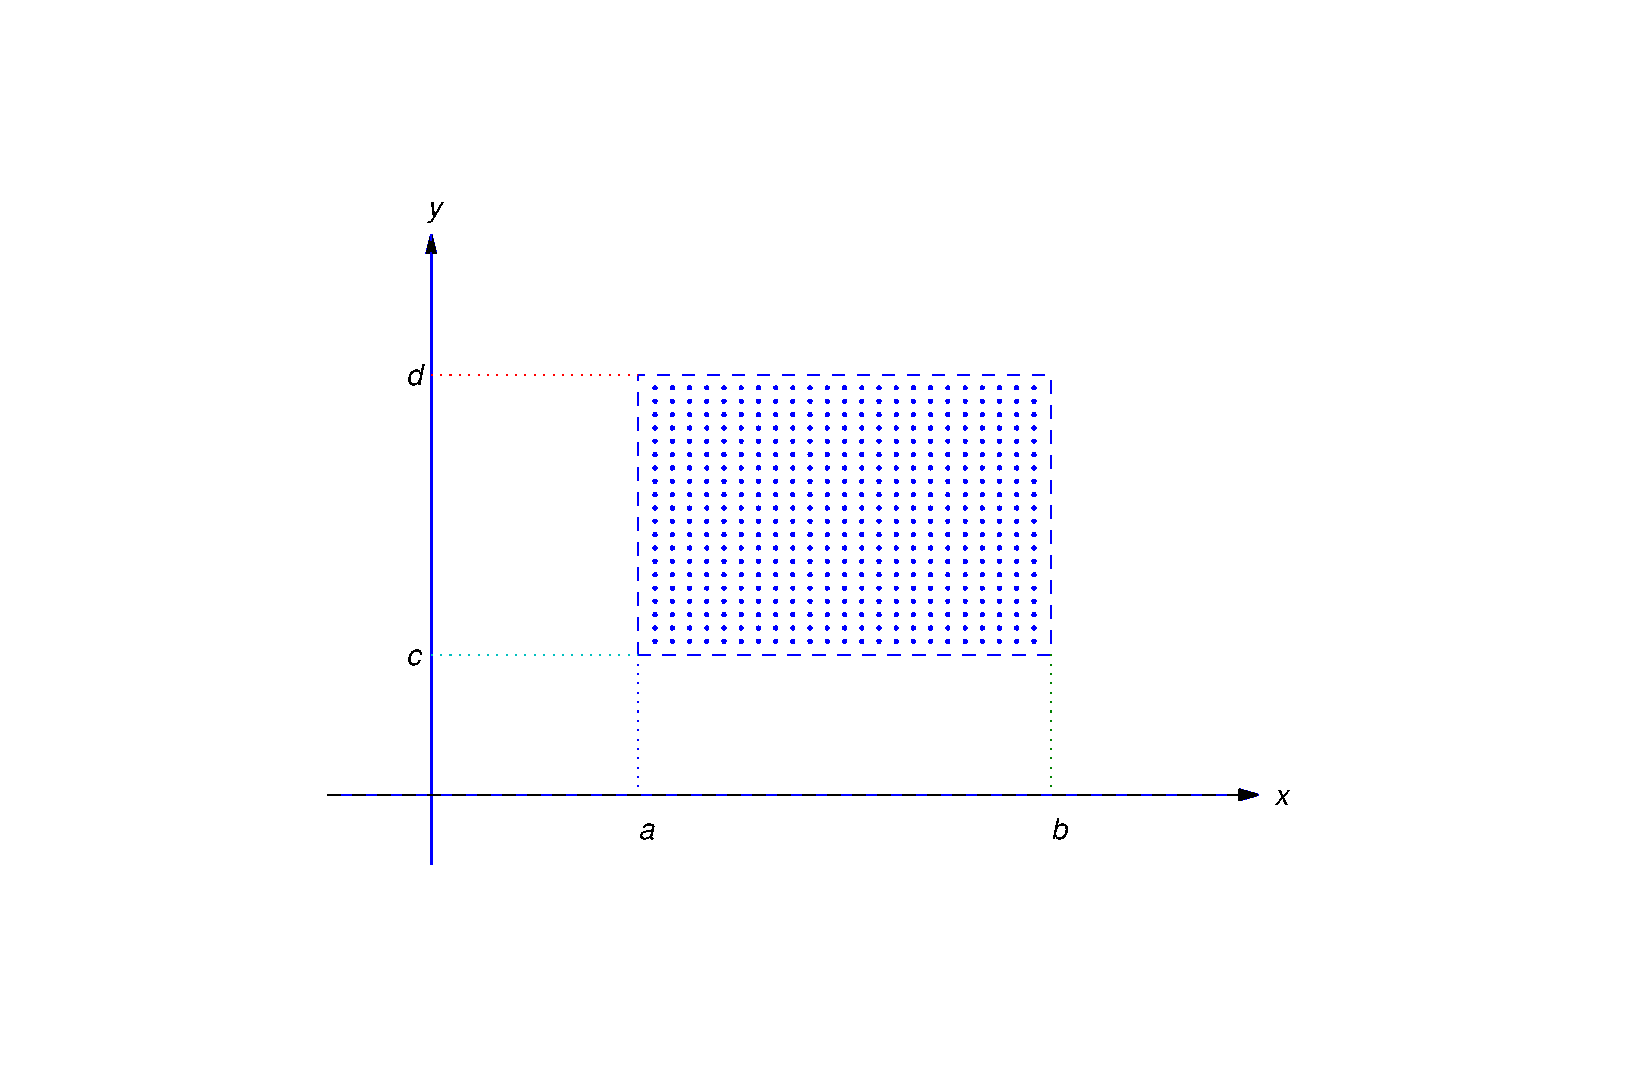
\includegraphics[bb=-78 148 689 643,width=5.67in,height=3.66in,keepaspectratio]{fig020301}}
\color{blue}
\vspace*{-35pt}
  \caption{An open rectangle}
  \label{figure:2.3.1}
\end{figure}

Some terminology:
 an {\color{blue}\it open rectangle $R$\/}
 is a set of points $(x,y)$ such that
$$
a<x<b\mbox{\quad  and \quad}c<y<d
$$
 (Figure~\ref{figure:2.3.1}).  We'll denote this set by
$R:  \{ a < x < b, c < y < d \}$.
 ``Open'' means that the
boundary rectangle (indicated by the dashed lines in
Figure~\ref{figure:2.3.1}) isn't  included in  $R$ .

The next theorem gives sufficient conditions for existence and
uniqueness of solutions of initial value problems for first order
nonlinear differential equations. We omit the proof, which is beyond
the scope of this book.

\begin{theorem}\color{blue} \label{thmtype:2.3.1} \mbox{}\newline
\vspace*{-5pt}
\begin{alist}
\item %(a)
 If  $f$ is continuous
on an open rectangle
$$
R:  \{ a < x < b, c < y < d \}
$$
 that contains $(x_0,y_0)$
then  the initial value problem
\begin{equation} \label{eq:2.3.1}
y'=f(x,y), \quad y(x_0)=y_0
\end{equation}
 has at least one solution  on some open subinterval
of  $(a,b)$ that contains $x_0$.

\item % (b)
 If  both $f$ and  $f_y$ are
 continuous on $R$ then \eqref{eq:2.3.1} has a unique
solution on some open subinterval  of $(a,b)$ that contains $x_0$.
\end{alist}
\end{theorem}

It's important to understand exactly what Theorem~\ref{thmtype:2.3.1}
says.

\begin{itemize}
\item \part{a} is an {\color{blue}\it existence theorem\/}. It guarantees that a
solution exists on some open interval that contains $x_0$, but provides
no information on how to find the solution, or to determine the open
interval on which it exists. Moreover, \part{a} provides no
information on the number of solutions that \eqref{eq:2.3.1} may have. It
leaves open the possibility that \eqref{eq:2.3.1} may have two or more
solutions that differ for values of $x$ arbitrarily close to $x_0$. We
will see in Example~\ref{example:2.3.6} that this can happen.

\item \part{b} is a {\color{blue}\it uniqueness theorem\/}. It guarantees that
\eqref{eq:2.3.1} has a unique solution on some open interval (a,b) that
contains $x_0$. However, if $(a,b)\ne(-\infty,\infty)$,
\eqref{eq:2.3.1} may have more than one solution on a larger interval
that contains $(a,b)$. For example, it may happen that $b<\infty$ and all
solutions have the same values on $(a,b)$, but two solutions $y_1$ and
$y_2$ are defined on some interval $(a,b_1)$ with $b_1>b$, and have
different values for $b<x<b_1$;   thus, the graphs of the $y_1$ and
$y_2$ ``branch off'' in different directions at $x=b$. (See
Example~\ref{example:2.3.7} and Figure~\ref{figure:2.3.3}). In this case,
continuity implies that $y_1(b)=y_2(b)$ (call their common value
$\overline y$), and  $y_1$ and $y_2$ are both solutions of the initial
value problem
\begin{equation} \label{eq:2.3.2}
y'=f(x,y),\quad y(b)=\overline y
\end{equation}
that differ on every open interval that contains $b$. Therefore
$f$ or $f_y$ must have a discontinuity at some point in each open
rectangle that contains $(b,\overline y)$, since if this were not so,
\eqref{eq:2.3.2} would have a unique solution on some open interval
that contains $b$. We leave it to you to give a similar analysis of the
case where $a>-\infty$.
 \end{itemize}

\begin{example}\label{example:2.3.1}
\rm   Consider  the initial value problem
\begin{equation} \label{eq:2.3.3}
y'={x^2-y^2 \over 1+x^2+y^2}, \quad y(x_0)=y_0.
\end{equation}
Since
$$
f(x,y)  = {x^2-y^2 \over 1+x^2+y^2}\mbox{\quad and \quad}
f_y(x,y)  =  -{2y(1+2x^2)\over (1+x^2+y^2)^2}
$$
are continuous for all $(x,y)$, Theorem~\ref{thmtype:2.3.1} implies that
if $(x_0,y_0)$ is arbitrary, then
\eqref{eq:2.3.3} has a unique solution on some open interval that contains
$x_0$.
\end{example}

\begin{example}\label{example:2.3.2}
\rm  Consider  the initial value problem
\begin{equation} \label{eq:2.3.4}
y'={x^2-y^2 \over x^2+y^2}, \quad y(x_0)=y_0.
\end{equation}
Here
$$
f(x,y)  =  {x^2-y^2 \over x^2+y^2}\mbox{\quad and \quad}
f_y(x,y)  =  \dst -{4x^2y \over (x^2+y^2)^2}
$$
are continuous everywhere except at $(0,0)$. If $(x_0,y_0)
\ne(0,0)$, there's an open rectangle $R$ that contains
$(x_0,y_0)$ that does not contain $(0,0)$. Since $f$ and $f_y$ are
continuous on $R$, Theorem~\ref{thmtype:2.3.1} implies that if
$(x_0,y_0)\ne(0,0)$ then
\eqref{eq:2.3.4}
has a unique solution on some open interval that contains $x_0$.
\end{example}

\begin{example}\label{example:2.3.3}
\rm  Consider the initial value problem
\begin{equation} \label{eq:2.3.5}
y'={x+y\over x-y},\quad y(x_0)=y_0.
\end{equation}
Here
$$
f(x,y)  =  {x+y\over x-y}\mbox{\quad and \quad}
f_y(x,y)  =  {2x\over (x-y)^2}
$$
are continuous everywhere except on the line $y=x$. If $y_0\ne x_0$,
there's an open rectangle $R$ that contains $(x_0,y_0)$ that
does not intersect the line $y=x$. Since $f$ and $f_y$ are continuous
on $R$, Theorem~\ref{thmtype:2.3.1} implies that if $y_0\ne x_0$,
\eqref{eq:2.3.5} has a unique solution on some open interval that contains
$x_0$.
\end{example}

\begin{example}\label{example:2.3.4}
\rm In Example~\ref{example:2.2.4} we saw that the
solutions of
\begin{equation} \label{eq:2.3.6}
y'=2xy^2
\end{equation}
are
 $$
y\equiv0\mbox{\quad and \quad} y=-{1 \over x^2+c},
$$
where $c$ is an arbitrary constant. In particular, this implies that
no solution of \eqref{eq:2.3.6} other than $y\equiv0$ can equal zero for
any value of $x$. Show that Theorem~\ref{thmtype:2.3.1}\part{b} implies
this.
\end{example}

\solution
We'll obtain a contradiction
by assuming that \eqref{eq:2.3.6} has a solution $y_1$ that equals
zero for some value of $x$, but isn't  identically zero. If $y_1$
has this property,  there's a point $x_0$ such that $y_1(x_0)=0$,
but $y_1(x)\ne0$ for some value of $x$ in every open interval that contains
$x_0$. This means that the initial value problem
\begin{equation} \label{eq:2.3.7}
y'=2xy^2,\quad y(x_0)=0
\end{equation}
has two solutions $y\equiv0$ and $y=y_1$ that differ for some value of
$x$ on every open interval that contains $x_0$. This contradicts
Theorem~\ref{thmtype:2.3.1}(b), since in \eqref{eq:2.3.6} the functions
$$
f(x,y)=2xy^2 \mbox{\quad and \quad} f_y(x,y)= 4xy.
$$
are both continuous
for all $(x,y)$, which implies that \eqref{eq:2.3.7} has a unique
solution on some open interval that contains $x_0$.

\begin{example}\label{example:2.3.5}
\rm  Consider the initial value problem
\begin{equation} \label{eq:2.3.8}
y' = {10\over 3}xy^{2/5}, \quad y(x_0) = y_0.
\end{equation}
\begin{alist}
\item %(a)
For what points $(x_0,y_0)$ does Theorem~\ref{thmtype:2.3.1}\part{a}
imply that
\eqref{eq:2.3.8} has a solution?

\item %(b)
For what points $(x_0,y_0)$ does Theorem~\ref{thmtype:2.3.1}\part{b}
imply that
\eqref{eq:2.3.8} has a  unique solution on some open interval that contains
$x_0$?
\end{alist}
\end{example}

\solutionpart{a} Since
$$
f(x,y) = {10\over 3}xy^{2/5}
$$
is continuous for all $(x,y)$,  Theorem~\ref{thmtype:2.3.1}
implies that \eqref{eq:2.3.8} has a solution for every $(x_0,y_0)$.

\solutionpart{b} Here
$$
f_y(x,y) = {4 \over 3}xy^{-3/5}
$$
is continuous for all $(x,y)$ with $y\ne 0$. Therefore, if $y_0\ne0$
there's an open rectangle on which both $f$ and $f_y$ are
continuous, and Theorem~\ref{thmtype:2.3.1} implies that \eqref{eq:2.3.8} has
a unique solution on some open interval that contains $x_0$.

If $y=0$ then $f_y(x,y)$ is undefined, and therefore discontinuous;
hence, Theorem~\ref{thmtype:2.3.1} does not apply to \eqref{eq:2.3.8} if
$y_0=0$.

\begin{example}\label{example:2.3.6}
\rm  Example~\ref{example:2.3.5} leaves open the possibility  that the
initial value problem
\begin{equation} \label{eq:2.3.9}
y'={10 \over 3}xy^{2/5}, \quad y(0)=0
\end{equation}
has more than one solution on every open interval that contains $x_0=0$.  Show
that this is true.
\end{example}

\solution
By inspection, $y\equiv0$ is a solution of the
differential equation
\begin{equation} \label{eq:2.3.10}
y'={10 \over 3} xy ^{2/5}.
\end{equation}
 Since $y\equiv0$ satisfies the initial condition $y(0)=0$,
it's a solution of \eqref{eq:2.3.9}.

Now suppose  $y$ is a solution of \eqref{eq:2.3.10} that isn't
identically zero.
 Separating variables in \eqref{eq:2.3.10} yields
$$
 y^{-2/5}y'={10 \over 3}x
$$
on any open interval where $y$ has no zeros.
 Integrating this and rewriting the arbitrary constant as $5c/3$ yields
$$
{5\over 3}y^{3/5} = {5\over 3}(x^2+c).
$$
Therefore
\begin{equation} \label{eq:2.3.11}
y = (x^2+c)^{5/3}.
\end{equation}

Since we divided by $y$ to separate variables in \eqref{eq:2.3.10}, our
derivation of \eqref{eq:2.3.11} is legitimate only on open intervals where $y$
has no zeros. However, \eqref{eq:2.3.11} actually defines $y$ for all $x$,
and differentiating \eqref{eq:2.3.11} shows that
$$
y'={10 \over 3}x(x^2+c)^{2/3}={10 \over 3}xy^{2/5},\,-\infty<x<\infty.
$$
Therefore \eqref{eq:2.3.11} satisfies \eqref{eq:2.3.10} on
$(-\infty,\infty)$
even if $c\le 0$, so that $y(\sqrt{|c|})=y(-\sqrt{|c|})=0$. In
particular, taking $c=0$ in \eqref{eq:2.3.11} yields
$$
y=x^{10/3}
$$
as a second solution of \eqref{eq:2.3.9}.
 Both solutions are defined on
$(-\infty,\infty)$, and they differ on every
open interval that contains $x_0=0$ (see Figure~\ref{figure:2.3.2}.)
In fact, there are {\color{blue}\it four\/} distinct solutions of
\eqref{eq:2.3.9}  defined on $(-\infty,\infty)$ that differ
from each other on every open interval that contains $x_0=0$.
  Can you identify the other two?

\begin{figure}[tbp]
  \centering
  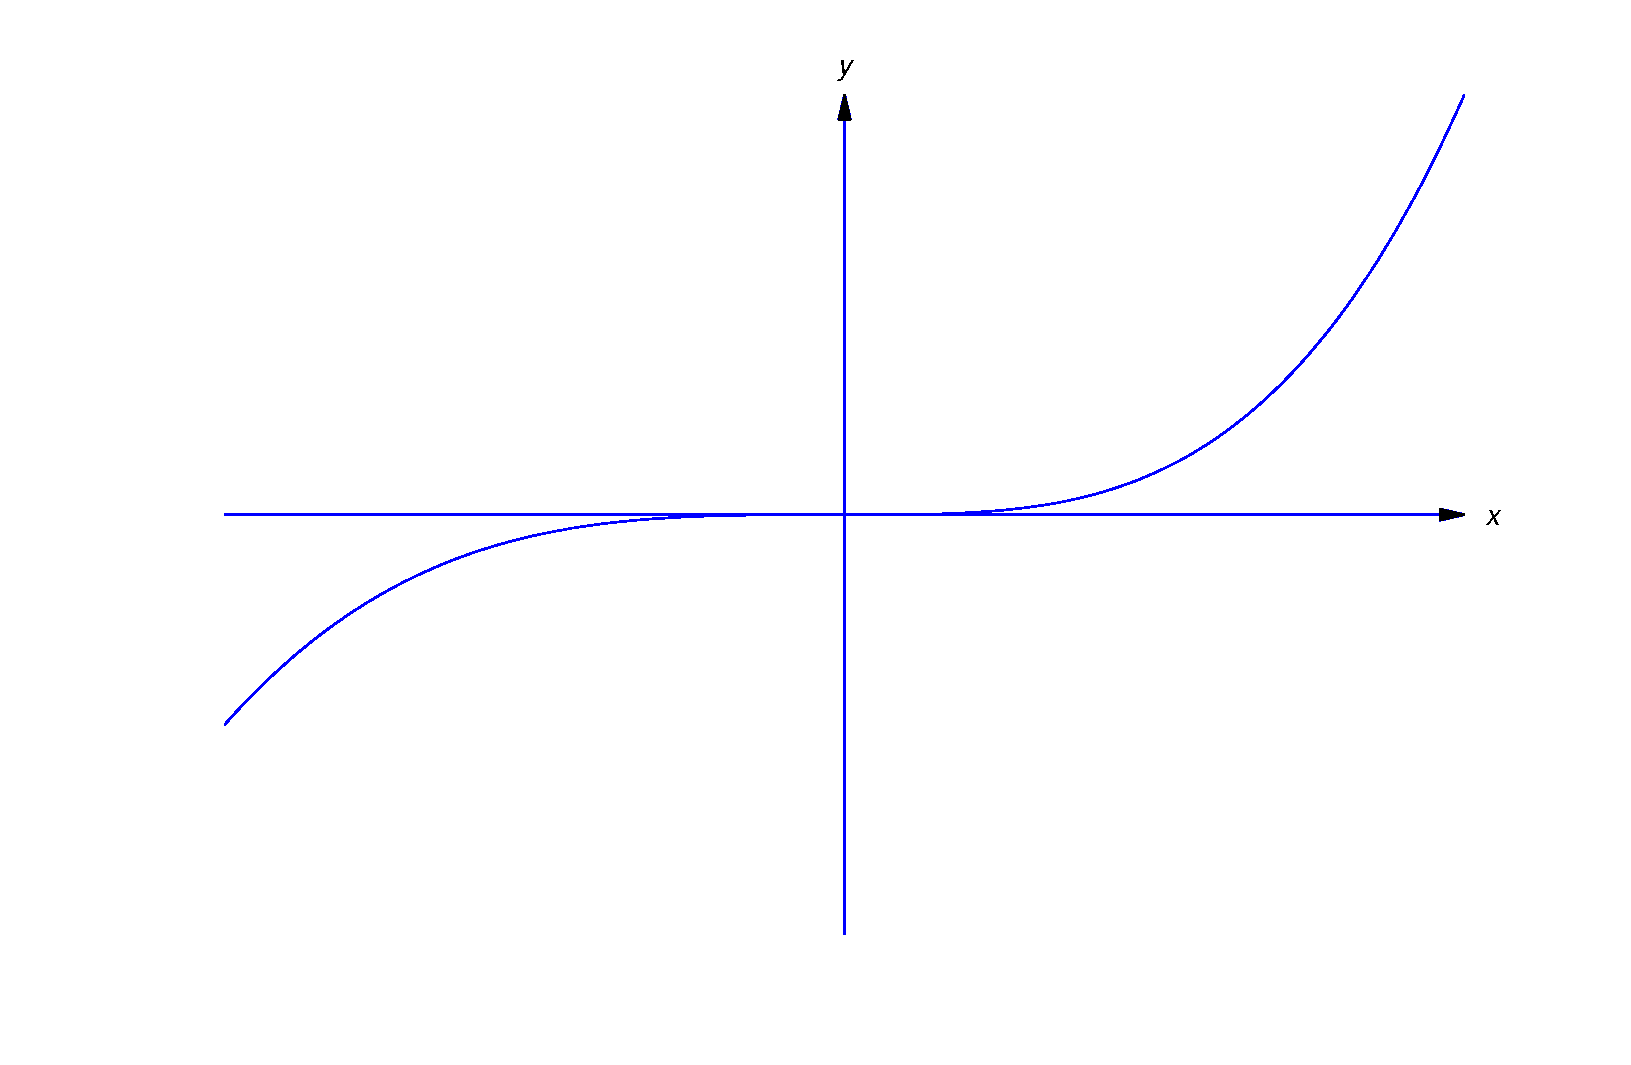
\includegraphics[bb=-78 148 689 643,width=5.67in,height=3.66in,keepaspectratio]{fig020302}
\color{blue}
\caption{Two solutions ($y=0$ and $y=x^{1/2}$) of \eqref{eq:2.3.9}  that
differ on every interval  containing $x_{0}=0$}
  \label{figure:2.3.2}
\end{figure}

\begin{example} \label{example:2.3.7}
\rm  From Example~\ref{example:2.3.5}, the initial value
problem
\begin{equation} \label{eq:2.3.12}
y'={10 \over 3}xy^{2/5}, \quad y(0)=-1
\end{equation}
 has a  unique solution on some open interval that contains $x_0=0$.
Find a solution and determine the largest open interval $(a,b)$ on
which it's unique.
\end{example}

\solution
Let $y$ be any solution of \eqref{eq:2.3.12}. Because of the initial
condition $y(0)=-1$ and the continuity of $y$, there's an open interval
$I$ that contains $x_0=0$ on which $y$ has no zeros, and is consequently
of the form \eqref{eq:2.3.11}. Setting $x=0$ and $y=-1$ in \eqref{eq:2.3.11}
yields $c=-1$, so
\begin{equation} \label{eq:2.3.13}
y=(x^2-1)^{5/3}
\end{equation}
for $x$  in $I$.
Therefore every solution of \eqref{eq:2.3.12} differs from zero
and is given by \eqref{eq:2.3.13} on $(-1,1)$; that is,
\eqref{eq:2.3.13} is the unique solution of \eqref{eq:2.3.12} on
$(-1,1)$.
 This is the largest open interval on which
\eqref{eq:2.3.12} has a unique solution. To see this, note that
\eqref{eq:2.3.13} is a solution of \eqref{eq:2.3.12} on $(-\infty,\infty)$.
From Exercise~2.2.~\hspace*{-3pt}\ref{exer:2.2.15}, there are infinitely many
other solutions
of \eqref{eq:2.3.12} that differ from \eqref{eq:2.3.13} on every open interval
larger than
$(-1,1)$. One such solution is
$$
y = \left\{ \begin{array}{cl}
(x^2-1)^{5/3}, & -1 \le x \le 1, \\[6pt]
0,             & |x|>1. \end{array} \right.
$$
(Figure \ref{figure:2.3.3}).

\begin{figure}[htbp]
\color{blue}
  \begin{minipage}[b]{0.5\linewidth}
    \centering
   \scalebox{.65}{
  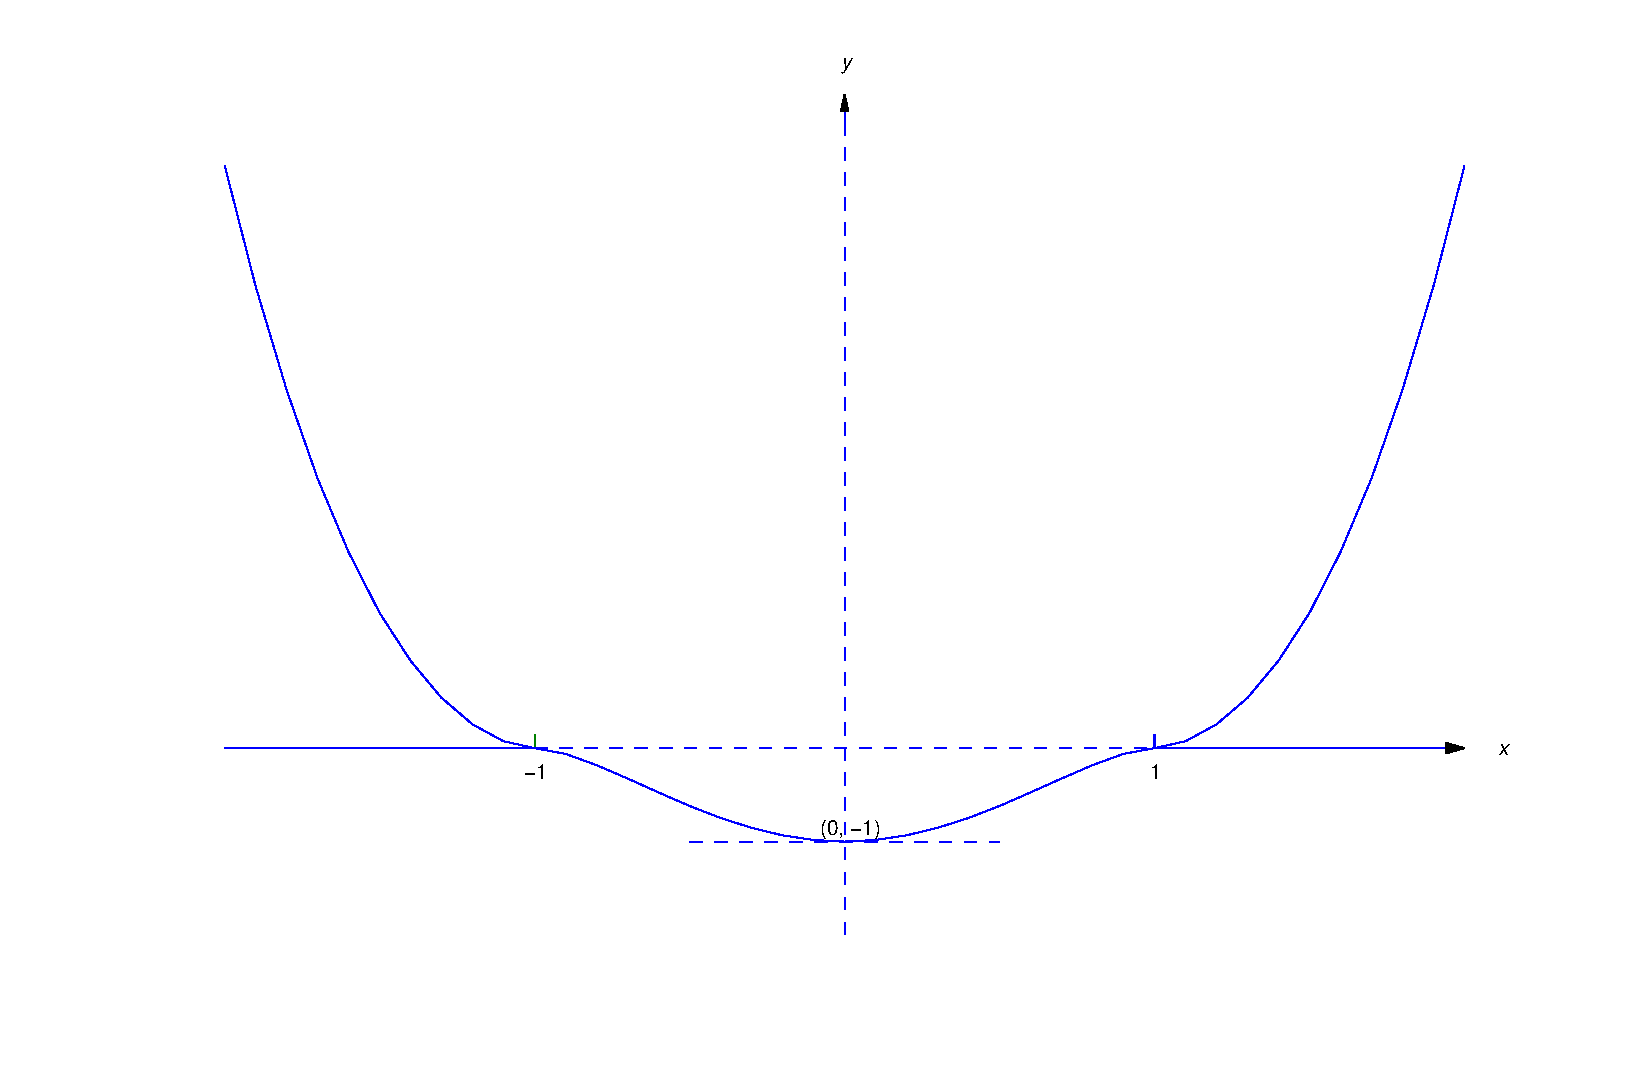
\includegraphics[bb=-78 148 689 643,width=5.67in,height=3.66in,keepaspectratio]{fig020303}}
\caption{ Two solutions of
\eqref{eq:2.3.12} on
$(-\infty,\infty)$ that coincide on $(-1,1)$, but on no larger open
interval}
  \label{figure:2.3.3}
  \end{minipage}
  \hspace{0.6cm}
  \begin{minipage}[b]{0.5\linewidth}
    \centering
   \scalebox{.65}{
  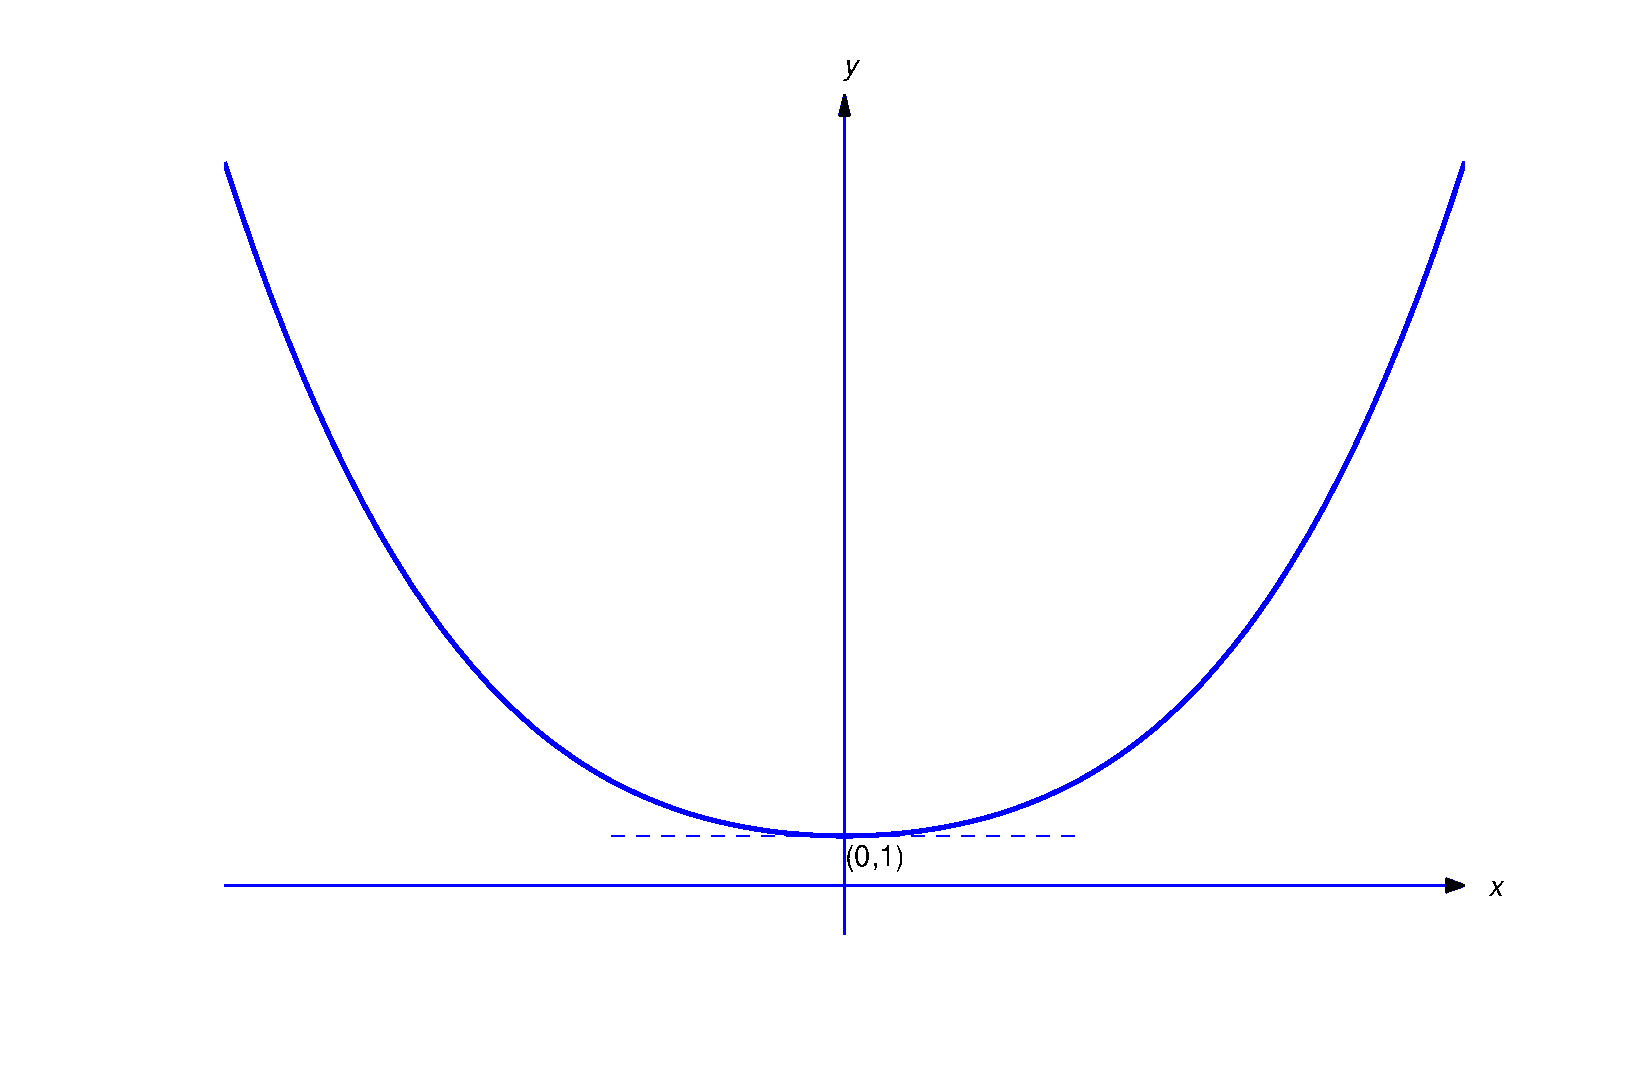
\includegraphics[bb=-78 148 689 643,width=5.67in,height=3.66in,keepaspectratio]{fig020304} }
  \caption{The unique solution of \eqref{eq:2.3.14}}
  \label{figure:2.3.4}
  \end{minipage}
\end{figure}

\begin{example}\label{example:2.3.8}
\rm  From Example~\ref{example:2.3.5}, the initial value
problem
\begin{equation} \label{eq:2.3.14}
y'={10 \over 3}xy^{2/5}, \quad y(0)=1
\end{equation}
 has a unique solution on some open interval that contains $x_0=0$.
Find the solution and determine the largest open interval on which it's
unique.
\end{example}

\solution
Let $y$ be any solution of \eqref{eq:2.3.14}. Because of the initial
condition $y(0)=1$ and the continuity of $y$, there's an open interval
$I$ that contains $x_0=0$ on which $y$ has no zeros, and is consequently
of the form \eqref{eq:2.3.11}. Setting $x=0$ and $y=1$ in \eqref{eq:2.3.11}
yields $c=1$, so
\begin{equation} \label{eq:2.3.15}
y=(x^2+1)^{5/3}
\end{equation}
for $x$ in $I$. Therefore every solution of \eqref{eq:2.3.14}
differs from zero and is given by \eqref{eq:2.3.15} on $(-\infty,\infty)$;
that is, \eqref{eq:2.3.15} is the unique solution of \eqref{eq:2.3.14} on
$(-\infty,\infty)$.
Figure~\ref{figure:2.3.4} shows the graph of this solution.

\exercises
 In Exercises \ref{exer:2.3.1}-\ref{exer:2.3.13} find all $(x_0,y_0)$ for
which Theorem~\ref{thmtype:2.3.1}
implies that the initial value problem $y'=f(x,y),\  y(x_0)=y_0$ has
\part{a}
a solution   \part{b} a  unique solution on some open interval that
contains
$x_0$.

\begin{exerciselist}

\begin{tabular}[t]{@{}p{168pt}@{}p{168pt}}
\item\label{exer:2.3.1} $\dst {y'={x^2+y^2
\over \sin
x}}$ &  \item\label{exer:2.3.2}\vspace*{10pt} $\dst
{y'={e^x+y \over x^2+y^2}}$ \end{tabular}

\begin{tabular}[t]{@{}p{168pt}@{}p{168pt}}
 \item\label{exer:2.3.3} $y'= \tan xy$
&  \item\label{exer:2.3.4} $\dst {y'={x^2+y^2
\over \ln xy}}$ \end{tabular}

\begin{tabular}[t]{@{}p{168pt}@{}p{168pt}}
 \item\label{exer:2.3.5} $y'=
(x^2+y^2)y^{1/3}$ &\  \item\label{exer:2.3.6}
\ $y'=2xy$ \end{tabular}

\begin{tabular}[t]{@{}p{168pt}@{}p{168pt}}
\vspace*{10pt} \item\label{exer:2.3.7} $\dst
{y'=\ln(1+x^2+y^2)}$
& \vspace*{4pt} \item\label{exer:2.3.8} $\dst {y'={2x+3y
\over x-4y}}$ \end{tabular}

\begin{tabular}[t]{@{}p{168pt}@{}p{168pt}}
 \item\label{exer:2.3.9} $\dst
{y'=(x^2+y^2)^{1/2}}$ &\item\label{exer:2.3.10}\  $y' =
x(y^2-1)^{2/3}$ \end{tabular}

\begin{tabular}[t]{@{}p{168pt}@{}p{168pt}}
\item\label{exer:2.3.11} $y'=(x^2+y^2)^2$
& \item\label{exer:2.3.12} $y'=(x+y)^{1/2}$
\end{tabular}

\item\label{exer:2.3.13}
$\dst {y'={\tan y \over x-1}}$

\item\label{exer:2.3.14}
Apply Theorem~\ref{thmtype:2.3.1} to the initial value problem
$$
y'+p(x)y = q(x), \quad y(x_0)=y_0
$$
for a linear equation, and compare the conclusions that can be drawn
from it to those that follow from Theorem 2.1.2.

\item\label{exer:2.3.15}
\begin{alist}
\item %(a)
Verify that the function
$$
y = \left\{ \begin{array}{cl}
(x^2-1)^{5/3}, & -1 < x < 1, \\[6pt]
0, & |x| \ge 1, \end{array} \right.
$$
is a solution of the initial value problem
$$
y'={10\over 3}xy^{2/5}, \quad y(0)=-1
$$
on $(-\infty,\infty)$. \hint{You'll need the definition $$
y'(\overline{x}) = \lim_{x \to \overline{x}} {y(x)-y(\overline{x})
\over x-\overline{x}} $$ to verify that $y$ satisfies the differential
equation at $\overline{x} = \pm 1$.}

\item %(b)
Verify that if $\epsilon_i=0$ or $1$ for $i=1$, $2$ and $a$, $b>1$, then
the function
$$
y = \left\{ \begin{array}{cl}
\epsilon_1(x^2-a^2)^{5/3}, & - \infty < x < -a, \\[6pt]
0, & -a \le x \le -1, \\[6pt]
(x^2-1)^{5/3}, &  -1 < x < 1, \\[6pt]
0, & 1 \le x \le b, \\[6pt]
\epsilon_2(x^2-b^2)^{5/3}, & b < x < \infty, \end{array} \right.
$$
is a solution of the initial value problem of \part{a} on
$(-\infty,\infty)$.
\end{alist}

\item\label{exer:2.3.16}
Use the ideas developed in Exercise~\ref{exer:2.3.15} to find
infinitely
many solutions  of the initial value problem
$$
y'=y^{2/5}, \quad y(0)=1
$$
on $(-\infty,\infty)$.

\item\label{exer:2.3.17}
 Consider the initial value
problem
$$
 y' = 3x(y-1)^{1/3}, \quad y(x_0) = y_0.
\eqno{\rm (A)}
$$

\begin{alist}
\item %(a)
For what points $(x_0,y_0)$ does Theorem~\ref{thmtype:2.3.1} imply that
(A) has a solution?
\item %(b)
 For what points $(x_0,y_0)$ does Theorem~\ref{thmtype:2.3.1} imply that
(A) has a  unique solution on some open interval
that contains  $x_0$?
\end{alist}

\item\label{exer:2.3.18}
Find nine solutions of the initial value problem
$$
y'=3x(y-1)^{1/3}, \quad y(0)=1
$$
that are all defined on $(-\infty,\infty)$ and differ from each other
for values of  $x$ in every open interval that contains $x_0=0$.

\item\label{exer:2.3.19}  From Theorem~\ref{thmtype:2.3.1}, the initial
value
problem
 $$
y'=3x(y-1)^{1/3}, \quad y(0)=9
$$
has a unique solution on an open interval that contains  $x_0=0$. Find the
solution and determine the largest open interval on which it's unique.

\item\label{exer:2.3.20}
\begin{alist}
\item %(a)
 From Theorem~\ref{thmtype:2.3.1},
the initial value problem
$$
 y'=3x(y-1)^{1/3}, \quad y(3)=-7
\eqno{\rm (A)}
$$
 has a unique solution on some open interval that contains $x_0=3$.
Determine
the largest such open interval, and find the solution on this interval.
\item %(b)
 Find infinitely many solutions of (A), all defined
on
$(-\infty,\infty)$.
\end{alist}

\item\label{exer:2.3.21}
Prove:
\begin{alist}
\item % ()
If
$$
f(x,y_0) = 0,\quad a<x<b,
\eqno{\rm (A)}
$$
and  $x_0$ is in  $(a,b)$,
then $y\equiv y_0$ is a solution of
$$
y'=f(x,y), \quad y(x_0)=y_0
$$
on $(a,b)$.
\item % (b)
If $f$ and $f_y$ are continuous on an open rectangle
that contains $(x_0,y_0)$ and (A) holds, no
solution of $y'=f(x,y)$ other than $y\equiv y_0$ can equal $y_0$ at
any point in $(a,b)$.
\end{alist}
\end{exerciselist}


\section{Transformation of Nonlinear Equations into Separable Equations}

\noindent
In Section~2.1 we found that the solutions of a linear nonhomogeneous equation
\[
  y'+p(x)y=f(x)
\]
are of the form $y=uy_{1}$, where $y_{1}$ is a nontrivial solution of the complementary equation
\begin{equation}
  \label{eq:2.4.1}y'+p(x)y=0
\end{equation}
and $u$ is a solution of
\[
  u'y_{1}(x)=f(x).
\]
Note that this last equation is separable, since it can be rewritten as
\[
  u'=\frac{f(x)}{y_{1}(x)}.
\]
In this section we'll consider nonlinear differential equations that are not separable to begin with, but can be solved in a similar fashion by writing their solutions in the form $y=uy_{1}$, where $y_{1}$ is a suitably chosen known function and $u$ satisfies a separable equation. We'll say in this case that we {\color{blue}\it transformed\/} the given equation into a separable equation.

\boxit{Bernoulli Equations}

\noindent
A
\href{https://mathshistory.st-andrews.ac.uk/Biographies/Bernoulli_Jacob/}{\color{blue}
\it Bernoulli equation}
is an equation of the form
\begin{equation}
  \label{eq:2.4.2}y'+p(x)y=f(x)y^{r},
\end{equation}
where $r$ can be any real number other than $0$ or $1$. (Note that \eqref{eq:2.4.2} is linear if and only if $r=0$ or $r=1$.) We can transform \eqref{eq:2.4.2} into a separable equation by variation of parameters: if $y_{1}$ is a nontrivial solution of \eqref{eq:2.4.1}, substituting $y=uy_{1}$ into \eqref{eq:2.4.2} yields
\[
  u'y_{1}+u(y_{1}'+p(x)y_{1})=f(x)(uy_{1})^{r},
\]
which is equivalent to the separable equation
\[
  u'y_{1}(x)=f(x)\left(y_{1}(x)\right)^{r}u^{r}\mbox{\quad or \quad}{\frac{u'}{u^{r}}}=f(x)\left(y_{1}(x)\right)^{r-1},
\]
since $y_{1}'+p(x)y_{1}=0$.

\begin{example}
  \label{example:2.4.1} \rm Solve the Bernoulli equation
  \begin{equation}
    \label{eq:2.4.3}y'-y=xy^{2}.
  \end{equation}
\end{example}

\solution Since $y_{1}=e^{x}$ is a solution of $y'-y=0$, we look for solutions of \eqref{eq:2.4.3} in the form $y=ue^{x}$, where
\[
  u'e^{x}=xu^{2}e^{2x}\mbox{\quad or, equivalently, \quad}u'=xu^{2}e^{x}.
\]
Separating variables yields
\[
  \frac{u'}{u^{2}}=xe^{x},
\]
and integrating yields
\[
  -\frac{1}{u}=(x-1)e^{x}+c.
\]
Hence,
\[
  u=-\frac{1}{(x-1)e^{x}+c}
\]
and
\[
  y=-\frac{1}{x-1+ce^{-x}}.
\]

Figure~\ref{eq:2.4.1} shows direction field and some integral curves of \eqref{eq:2.4.3}.

\begin{figure}[tbp]
  \centering
  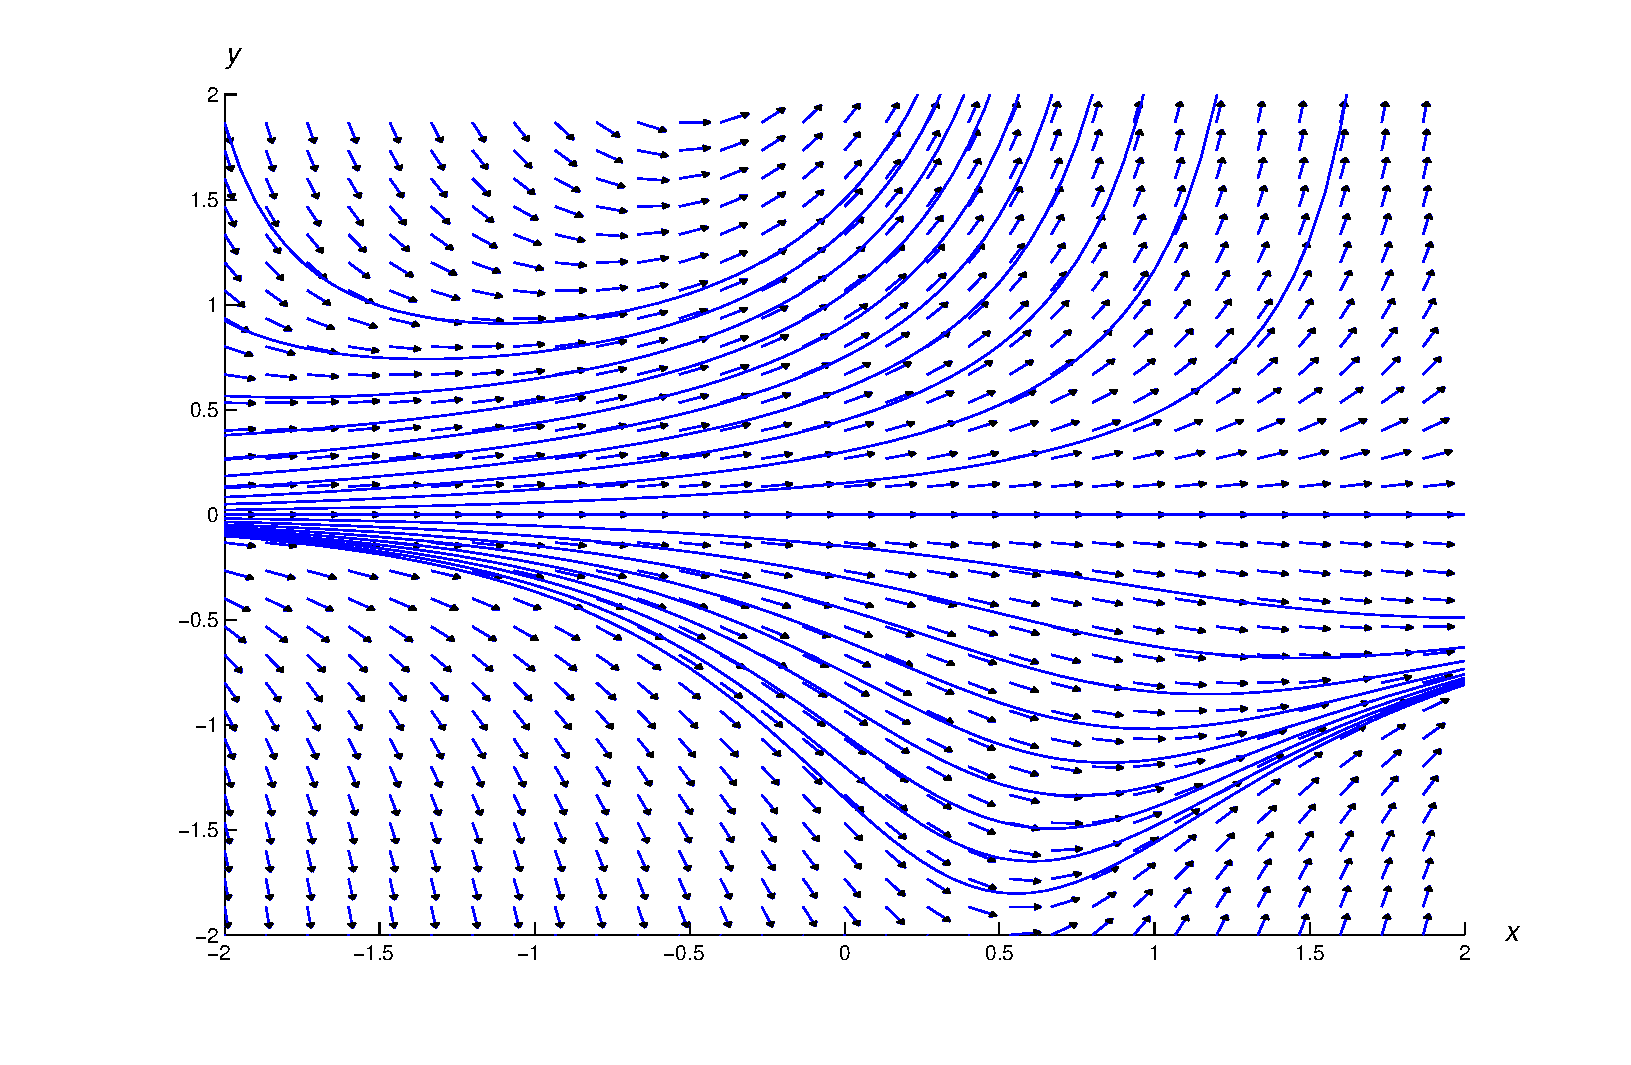
\includegraphics[bb=-78 148 689 643, width=5.67in, height=3.66in, keepaspectratio]{fig020401}
  \color{blue}
  \caption{A direction field and integral curves for $y'-y=xy^{2}$}
  \label{figure:2.4.1}
\end{figure}

\boxit{Other Nonlinear Equations That Can be Transformed Into Separable Equations}

\noindent
We've seen that the nonlinear Bernoulli equation can be transformed into a separable equation by the substitution $y=uy_{1}$ if $y_{1}$ is suitably chosen. Now let's discover a sufficient condition for a nonlinear first order differential equation
\begin{equation}
  \label{eq:2.4.4}y'=f(x,y)
\end{equation}
to be transformable into a separable equation in the same way. Substituting $y=uy_{1}$ into \eqref{eq:2.4.4} yields
\[
  u'y_{1}(x)+uy_{1}'(x)=f(x,uy_{1}(x)),
\]
which is equivalent to
\begin{equation}
  \label{eq:2.4.5}u'y_{1}(x)=f(x,uy_{1}(x))-uy_{1}'(x).
\end{equation}
If
\[
  f(x,uy_{1}(x))=q(u)y_{1}'(x)
\]
for some function $q$, then \eqref{eq:2.4.5} becomes
\begin{equation}
  \label{eq:2.4.6}u'y_{1}(x)=(q(u)-u)y_{1}'(x),
\end{equation}
which is separable. After checking for constant solutions $u\equiv u_{0}$ such that $q(u_{0})=u_{0}$, we can separate variables to obtain
\[
  \frac{u'}{q(u)-u}=\frac{y_{1}'(x)}{y_{1}(x)}.
\]

\boxit{Homogeneous Nonlinear Equations}

\noindent
In the text we'll consider only the most widely studied class of equations for which the method of the preceding paragraph works. Other types of equations appear in Exercises~\ref{exer:2.4.44}--\ref{exer:2.4.51}.

The differential equation \eqref{eq:2.4.4} is said to be {\color{blue}\it homogeneous\/} if $x$ and $y$ occur in $f$ in such a way that $f(x,y)$ depends only on the ratio $y/x$; that is, \eqref{eq:2.4.4} can be written as
\begin{equation}
  \label{eq:2.4.7}y'=q(y/x),
\end{equation}
where $q=q(u)$ is a function of a single variable. For example,
\[
  y'=\frac{y+xe^{-y/x}}{x}=\frac{y}{x}+e^{-y/x}
\]
and
\[
  y'=\frac{y^{2}+xy-x^{2}}{x^{2}}=\left(\frac{y}{x}\right)^{2}+\frac{y}{x}-1
\]
are of the form \eqref{eq:2.4.7}, with
\[
  q(u)=u+e^{-u}\mbox{\quad and \quad}q(u)=u^{2}+u-1,
\]
respectively. The general method discussed above can be applied to \eqref{eq:2.4.7} with $y_{1}=x$ (and therefore $y_{1}'=1$). Thus, substituting $y=ux$ in \eqref{eq:2.4.7} yields
\[
  u'x+u=q(u),
\]
and separation of variables (after checking for constant solutions $u\equiv u_{0}$ such that $q(u_{0})=u_{0}$) yields
\[
  \frac{u'}{q(u)-u}=\frac{1}{x}.
\]

Before turning to examples, we point out something that you may've have already noticed: the definition of {\color{blue}\it homogeneous equation\/} given here isn't the same as the definition given in Section~2.1, where we said that a linear equation of the form
\[
  y'+p(x)y=0
\]
is homogeneous. We make no apology for this inconsistency, since we didn't create it historically, {\color{blue}\it homogeneous\/} has been used in these two inconsistent ways. The one having to do with linear equations is the most important. This is the only section of the book where the meaning defined here will apply.

Since $y/x$ is in general undefined if $x=0$, we'll consider solutions of nonhomogeneous equations only on open intervals that do not contain the point $x=0$.

\begin{example}
  \label{example:2.4.2}\rm Solve
  \begin{equation}
    \label{eq:2.4.8}y'=\frac{y+xe^{-y/x}}{x}.
  \end{equation}
\end{example}

\solution Substituting $y=ux$ into \eqref{eq:2.4.8} yields
\[
  u'x+u=\frac{ux+xe^{-ux/x}}{x}=u+e^{-u}.
\]
Simplifying and separating variables yields
\[
  e^{u}u'=\frac{1}{x}.
\]
Integrating yields $e^{u}=\ln|x|+c$. Therefore $u=\ln(\ln|x|+c)$ and $y=ux=x\ln(\ln|x|+c)$.

Figure~\ref{figure:2.4.2} shows a direction field and integral curves for \eqref{eq:2.4.8}.

\begin{figure}[H]
  \centering
  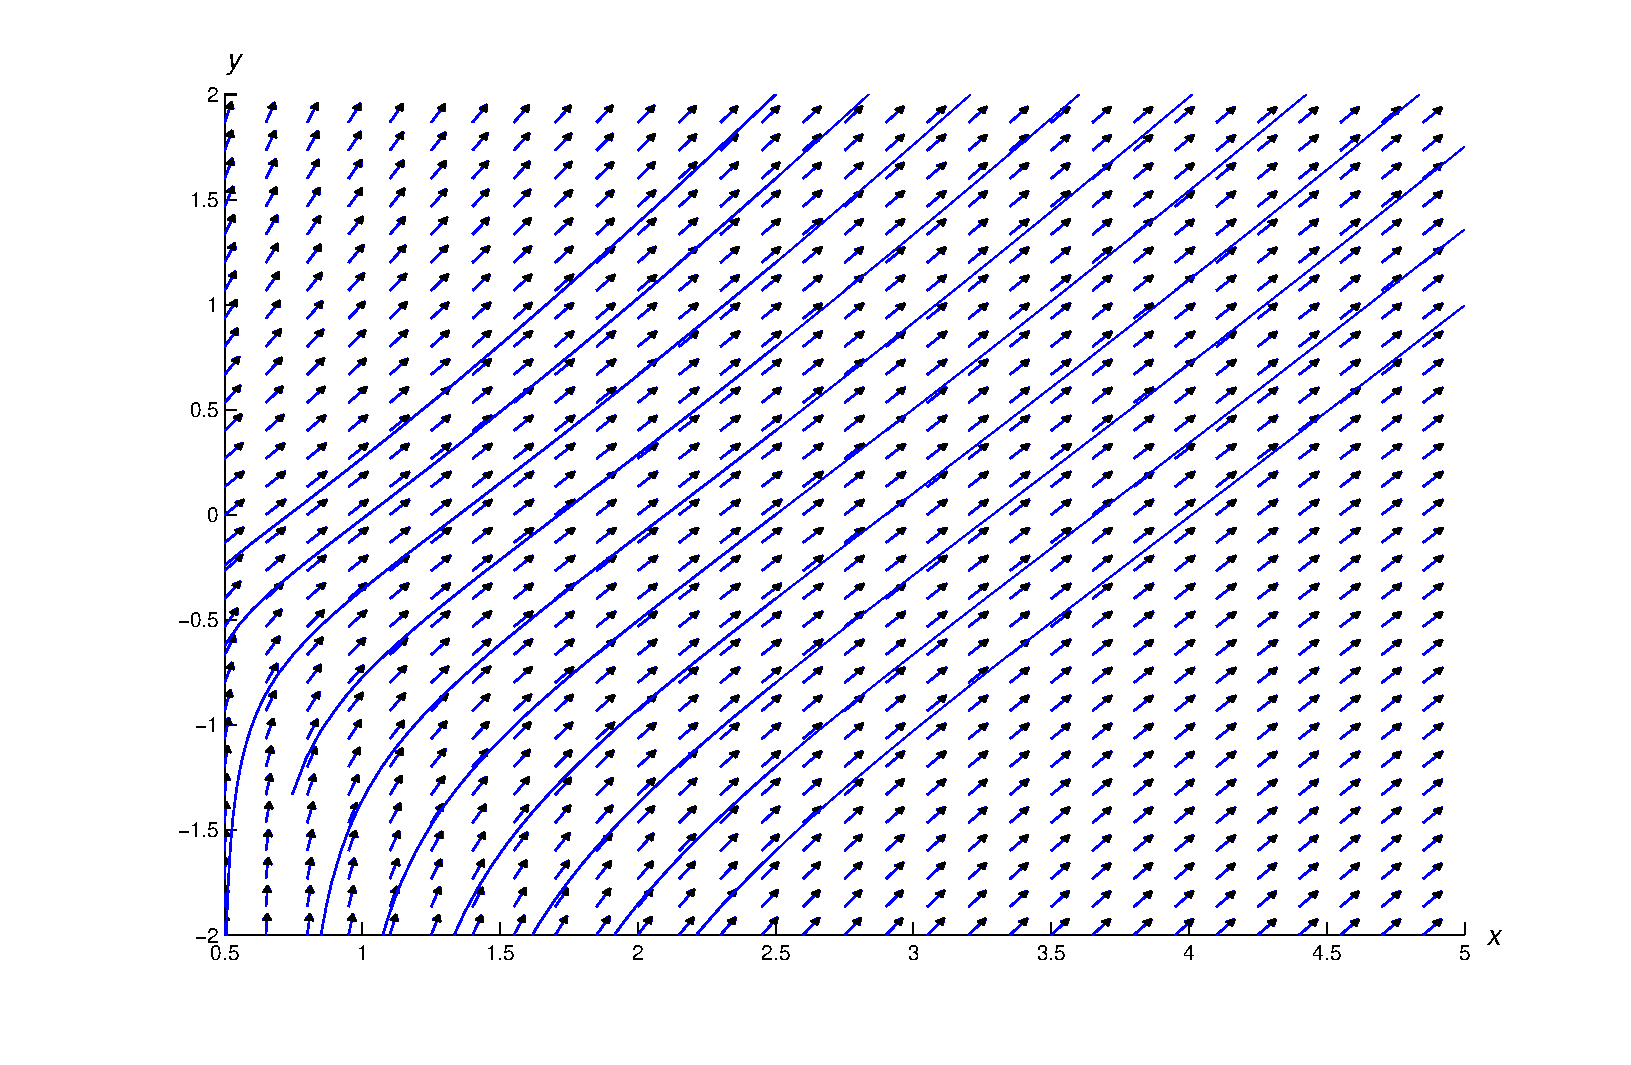
\includegraphics[bb=-78 148 689 643, width=5.67in, height=3.66in, keepaspectratio]{fig020402}
  \color{blue}
  \caption{A direction field and some integral curves for $y'=\dst{\frac{y+xe^{-y/x}}{x}}$}
  \label{figure:2.4.2}
\end{figure}

\begin{example}
  \label{example:2.4.3}\rm \mbox{}
  \newline
  \begin{alist}
    \item % (a)
    Solve
    \begin{equation}
      \label{eq:2.4.9}x^{2}y'=y^{2}+xy-x^{2}.
    \end{equation}

    \item % (b)
    Solve the initial value problem
    \begin{equation}
      \label{eq:2.4.10}x^{2}y'=y^{2}+xy-x^{2},\quad y(1)=2.
    \end{equation}
  \end{alist}
\end{example}

\solutionpart{a} We first find solutions of \eqref{eq:2.4.9} on open intervals that don't contain $x=0$. We can rewrite \eqref{eq:2.4.9} as
\[
  y'=\frac{y^{2}+xy-x^{2}}{x^{2}}
\]
for $x$ in any such interval. Substituting $y=ux$ yields
\[
  u'x+u=\frac{(ux)^{2}+x(ux)-x^{2}}{x^{2}}=u^{2}+u-1,
\]
so
\begin{equation}
  \label{eq:2.4.11}u'x=u^{2}-1.
\end{equation}
By inspection this equation has the constant solutions $u\equiv1$ and $u\equiv-1$. Therefore $y=x$ and $y=-x$ are solutions of \eqref{eq:2.4.9}. If $u$ is a solution of \eqref{eq:2.4.11} that doesn't assume the values $\pm1$ on some interval, separating variables yields
\[
  \frac{u'}{u^{2}-1}=\frac{1}{x},
\]
or, after a partial fraction expansion,
\[
  \frac{1}{2}\left[\frac{1}{u-1}-\frac{1}{u+1}\right]u'= \frac{1}{x}.
\]
Multiplying by 2 and integrating yields
\[
  \ln\left|\frac{u-1}{u+1}\right|=2\ln|x|+k,
\]
or
\[
  \left|\frac{u-1}{u+1}\right|=e^{k}x^{2},
\]
which holds if
\begin{equation}
  \label{eq:2.4.12}\frac{u-1}{u+1}=cx^{2}
\end{equation}
where $c$ is an arbitrary constant. Solving for $u$ yields
\[
  u=\frac{1+cx^{2}}{1-cx^{2}}.
\]

\begin{figure}[htbp]
  \color{blue}
  \begin{minipage}[b]{0.5\linewidth}
    \centering
    \scalebox{.6}{
    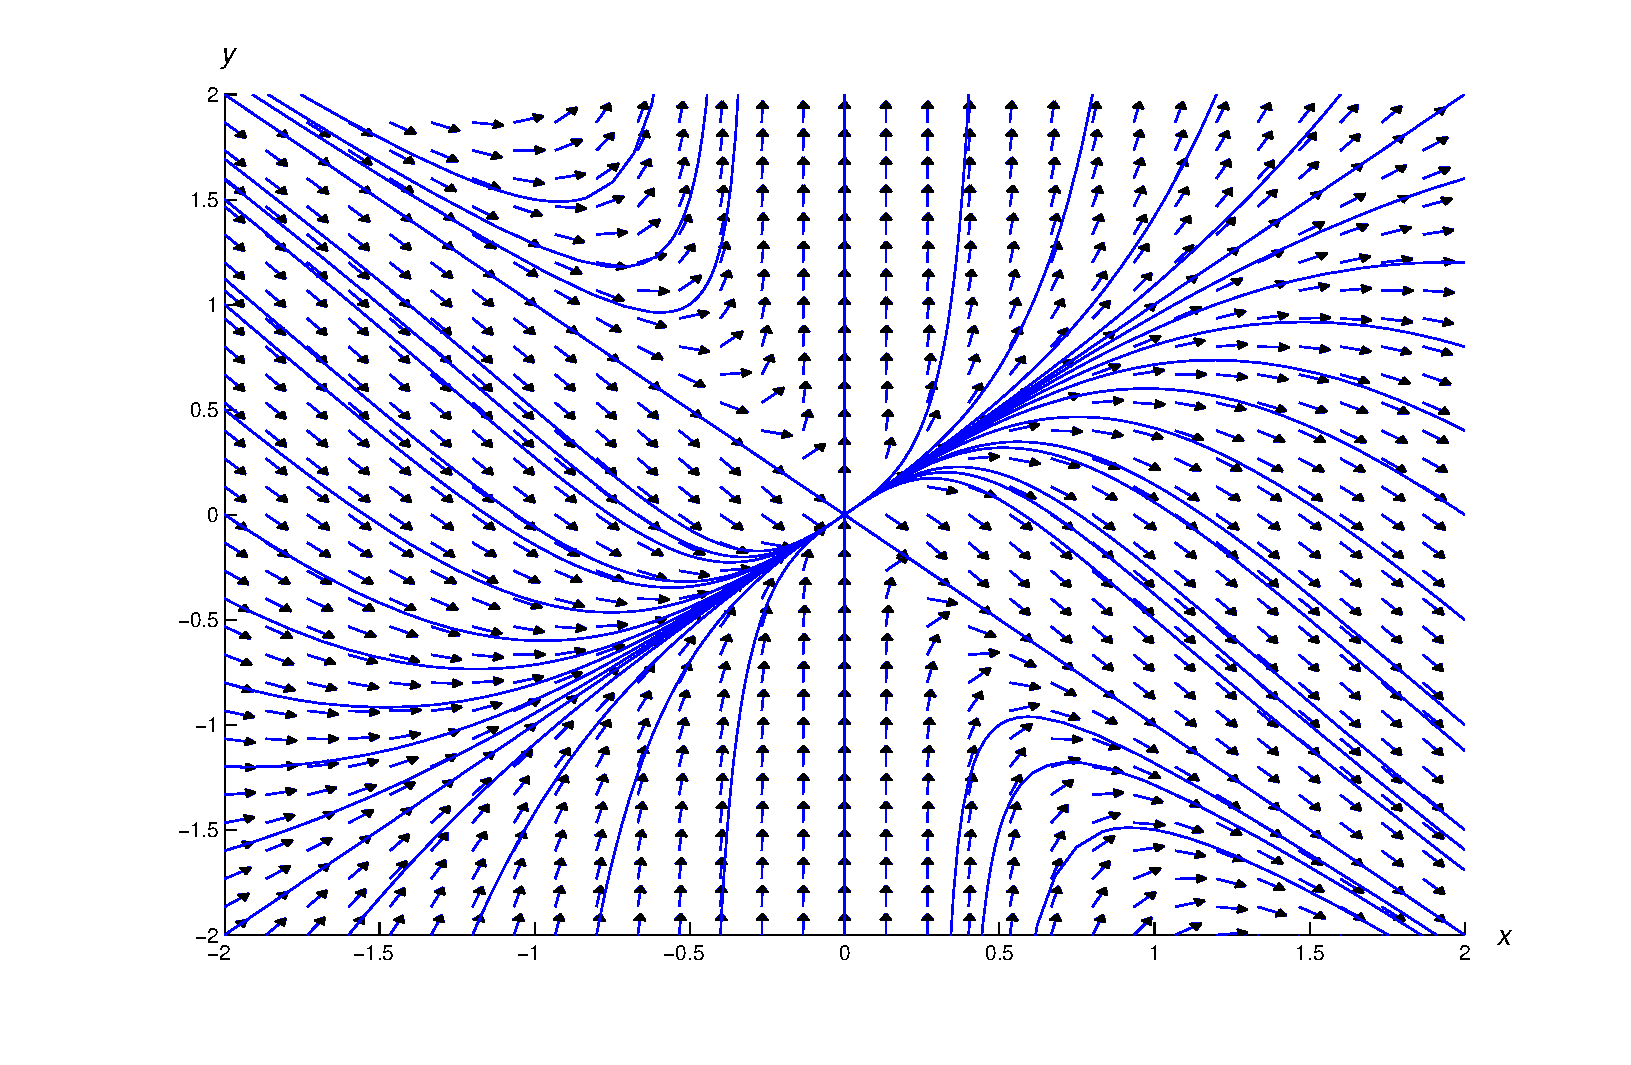
\includegraphics[bb=-78 148 689 643, width=5.67in, height=3.66in, keepaspectratio]{fig020403}
    }
    \color{blue}
    \caption{A direction field and integral curves for $x^{2}y'=y^{2}+xy-x^{2}$}
    \label{figure:2.4.3}
  \end{minipage}
  \hspace{0.6cm}
  \begin{minipage}[b]{0.5\linewidth}
    \centering
    \scalebox{.7}{
    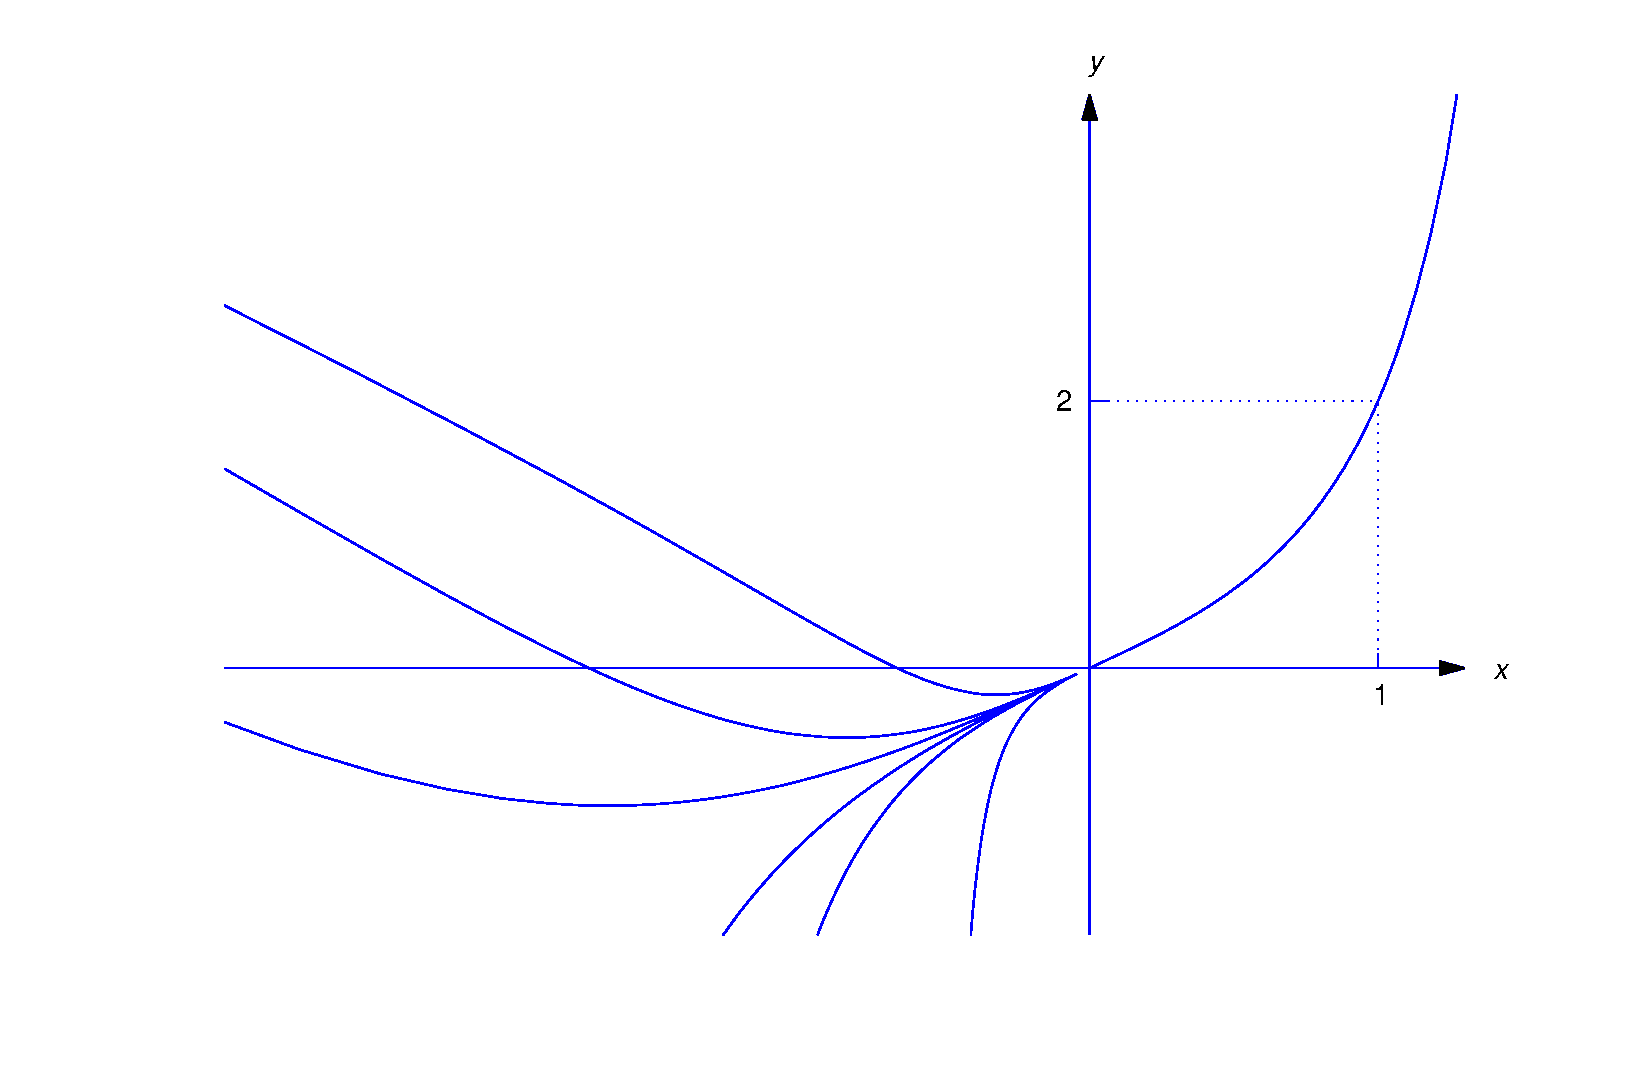
\includegraphics[bb=-78 148 689 643, width=5.67in, height=3.66in, keepaspectratio]{fig020404}}
    \caption{Solutions of $x^{2}y'=y^{2}+xy-x^{2}$,\; $y(1)=2$}
    \label{figure:2.4.4}
  \end{minipage}
\end{figure}

\noindent
Therefore
\begin{equation}
  \label{eq:2.4.13}y=ux=\frac{x(1+cx^{2})}{1-cx^{2}}
\end{equation}
is a solution of \eqref{eq:2.4.10} for any choice of the constant $c$. Setting $c=0$ in \eqref{eq:2.4.13} yields the solution $y=x$. However, the solution $y=-x$ can't be obtained from \eqref{eq:2.4.13}. Thus, the solutions of \eqref{eq:2.4.9} on intervals that don't contain $x=0$ are $y=-x$ and functions of the form \eqref{eq:2.4.13}.

The situation is more complicated if $x=0$ is the open interval. First, note that $y=-x$ satisfies \eqref{eq:2.4.9} on $(-\infty,\infty)$. If $c_{1}$ and $c_{2}$ are arbitrary constants, the function
\begin{equation}
  \label{eq:2.4.14}y=\left\{
  \begin{array}{ll}
    \dst\frac{x(1+c_{1}x^{2})}{1-c_{1}x^{2}},        & a<x<0,    \\
    [2\jot]\dst\frac{x(1+c_{2}x^{2})}{1-c_{2}x^{2}}, & 0\le x<b,
  \end{array}\right.
\end{equation}
is a solution of \eqref{eq:2.4.9} on $(a,b)$, where
\[
  a=\left\{
  \begin{array}{cl}
    -\dst\frac{1}{\sqrt{c_{1}}} & \mbox{ if }c_{1}>0,   \\
    -\infty                     & \mbox{ if }c_{1}\le0,
  \end{array}\right.\mbox{\quad and \quad}b=\left\{
  \begin{array}{cl}
    \dst\frac{1}{\sqrt{c_{2}}} & \mbox{ if }c_{2}>0,   \\
    \infty                     & \mbox{ if }c_{2}\le0.
  \end{array}\right.
\]
We leave it to you to verify this. To do so, note that if $y$ is any function of the form \eqref{eq:2.4.13} then $y(0)=0$ and $y'(0)=1$.

Figure~\ref{figure:2.4.3} shows a direction field and some integral curves for \eqref{eq:2.4.9}.

\solutionpart{b} We could obtain $c$ by imposing the initial condition $y(1)=2$ in \eqref{eq:2.4.13}, and then solving for $c$. However, it's easier to use \eqref{eq:2.4.12}. Since $u=y/x$, the initial condition $y(1)=2$ implies that $u(1)=2$. Substituting this into \eqref{eq:2.4.12} yields $c=1/3$. Hence, the solution of \eqref{eq:2.4.10} is
\[
  y=\frac{x(1+x^{2}/3)}{1-x^{2}/3}.
\]
The interval of validity of this solution is $(-\sqrt{3},\sqrt{3})$. However, the largest interval on which \eqref{eq:2.4.10} has a unique solution is $(0,\sqrt{3})$. To see this, note from \eqref{eq:2.4.14} that any function of the form
\begin{equation}
  \label{eq:2.4.15}y=\left\{
  \begin{array}{ll}
    \dst\frac{x(1+cx^{2})}{1-cx^{2}},   & a<x\le0,         \\[2\jot]
    \dst\frac{x(1+x^{2}/3)}{1-x^{2}/3}, & 0\le x<\sqrt{3},
  \end{array}\right.
\end{equation}
is a solution of \eqref{eq:2.4.10} on $(a,\sqrt{3})$, where $a=-1/\sqrt{c}$ if $c>0$ or $a=-\infty$ if $c\le0$. (Why doesn't this contradict Theorem~\ref{thmtype:2.3.1}?)

Figure~\ref{figure:2.4.4} shows several solutions of the initial value problem~\eqref{eq:2.4.10}. Note that these solutions coincide on $(0,\sqrt{3})$.

In the last two examples we were able to solve the given equations explicitly. However, this isn't always possible, as you'll see in the exercises.

\exercises In Exercises~\ref{exer:2.4.1}--\ref{exer:2.4.4} solve the given Bernoulli equation.

\begin{exerciselist}
  \begin{tabular}[t]{@{}p{168pt}@{}p{168pt}}
    \item\label{exer:2.4.1} $y'+y=y^{2}$ &
    \item\label{exer:2.4.2} $\dst{7xy'-2y=-\frac{x^{2}}{y^{6}}}$
  \end{tabular}

  \begin{tabular}[t]{@{}p{168pt}@{}p{168pt}}
    \item\label{exer:2.4.3} $x^{2}y'+2y=2e^{1/x}y^{1/2}$ &

    \item\label{exer:2.4.4} \vspace*{-5pt}$\dst{(1+x^{2})y'+2xy =\frac{1}{(1+x^{2})y}}$
  \end{tabular}

  \exercisetext{In Exercises~\ref{exer:2.4.5} and \ref{exer:2.4.6} find all solutions. Also, plot a direction field and some integral curves on the indicated rectangular region.}

  \item\label{exer:2.4.5} \CGex $y'-xy=x^{3}y^{3};\quad\{-3\le x\le3,\-2\le y\ge2\}$

  \item\label{exer:2.4.6} \CGex $\dst{y'-\frac{1+x}{3x}y=y^{4}};\quad\{-2\le x\le2,-2\le y\le2\}$

  \exercisetext{In Exercises~\ref{exer:2.4.7}--\ref{exer:2.4.11} solve the initial value problem.}

  \item\label{exer:2.4.7} $y'-2y=xy^{3},\quad y(0)=2\sqrt{2}$

  \item\label{exer:2.4.8} $y'-xy=xy^{3/2},\quad y(1)=4$

  \item\label{exer:2.4.9} $xy'+y=x^{4}y^{4},\quad y(1)=1/2$

  \item\label{exer:2.4.10} $y'-2y=2y^{1/2},\quad y(0)=1$

  \item\label{exer:2.4.11} $\dst{y'-4y=\frac{48x}{y^{2}},\quad y(0)=1}$

  \exercisetext{In Exercises~\ref{exer:2.4.12} and \ref{exer:2.4.13} solve the initial value problem and graph the solution.}

  \item\label{exer:2.4.12} \CGex $x^{2}y'+2xy=y^{3},\quad y(1)=1/\sqrt{2}$

  \item\label{exer:2.4.13} \CGex $y'-y=xy^{1/2},\quad y(0)=4$

  \item\label{exer:2.4.14} You may have noticed that the logistic equation
  \[
    P'=aP(1-\alpha P)
  \]
  from Verhulst's model for population growth can be written in Bernoulli form as
  \[
    P'-aP=-a\alpha P^{2}.
  \]
  This isn't particularly interesting, since the logistic equation is separable, and therefore solvable by the method studied in Section~2.2. So let's consider a more complicated model, where $a$ is a positive constant and $\alpha$ is a positive continuous function of $t$ on $[0,\infty)$. The equation for this model is
  \[
    P'-aP=-a\alpha(t)P^{2},
  \]
  a non-separable Bernoulli equation.
  \begin{alist}
    \item % (a)
    Assuming that $P(0)=P_{0}>0$, find $P$ for $t>0$. \hint{Express your result in terms of the integral $\int_{0}^{t}\alpha(\tau)e^{a\tau}\,d\tau$.}

    \item % (b)
    Verify that your result reduces to the known results for the Malthusian model where $\alpha=0$, and the Verhulst model where $\alpha$ is a nonzero constant.

    \item % (c)
    Assuming that
    \[
      \lim_{t\to\infty}e^{-at}\int_{0}^{t}\alpha(\tau)e^{a\tau}\,d\tau=L
    \]
    exists (finite or infinite), find $\lim_{t\to\infty}P(t)$.
  \end{alist}

  \exercisetext{In Exercises~\ref{exer:2.4.15}--\ref{exer:2.4.18} solve the equation explicitly.}

  \begin{tabular}[t]{@{}p{168pt}@{}p{168pt}}
    \item\label{exer:2.4.15} $y'=\dst\frac{y+x}{x}$ & \vspace*{5pt}
    \item\label{exer:2.4.16} $y'=\dst\frac{y^{2}+2xy}{x^{2}}$
  \end{tabular}

  \begin{tabular}[t]{@{}p{168pt}@{}p{168pt}}
    \item\label{exer:2.4.17} $xy^{3}y'=y^{4}+x^{4}$ &
    \item\label{exer:2.4.18} $y'=\dst\frac{y}{x}+\sec\frac{y}{x}$
  \end{tabular}

  \exercisetext{In Exercises~\ref{exer:2.4.19}-\ref{exer:2.4.21} solve the equation explicitly. Also, plot a direction field and some integral curves on the indicated rectangular region.}

  \item\label{exer:2.4.19} \CGex $x^{2}y'=xy+x^{2}+y^{2};\quad\{-8\le x\le8,-8\le y\le8\}$

  \item\label{exer:2.4.20} \CGex $xyy'=x^{2}+2y^{2};\quad\{-4\le x\le4,-4\le y\le4\}$

  \item\label{exer:2.4.21} \CGex $y'=\dst\frac{2y^{2}+x^{2}e^{-(y/x)^{2}}}{2xy}; \quad\{-8\le x\le8,-8\le y\le8\}$

  \exercisetext{In Exercises~\ref{exer:2.4.22}--\ref{exer:2.4.27} solve the initial value problem.}

  \item\label{exer:2.4.22} $y'=\dst\frac{xy+y^{2}}{x^{2}}, \quad y(-1)=2$

  \item\label{exer:2.4.23} $y'=\dst\frac{x^{3}+y^{3}}{xy^{2}},\quad y(1)=3$

  \item\label{exer:2.4.24} $xyy'+x^{2}+y^{2}=0,\quad y(1)=2$

  \item\label{exer:2.4.25} $y'=\dst\frac{y^{2}-3xy-5x^{2}}{x^{2}},\quad y(1)=-1$

  \item\label{exer:2.4.26} $x^{2}y'=2x^{2}+y^{2}+4xy,\quad y(1)=1$

  \item\label{exer:2.4.27} $xyy'=3x^{2}+4y^{2},\quad y(1)=\sqrt{3}$

  \exercisetext{In Exercises~\ref{exer:2.4.28}--\ref{exer:2.4.34} solve the given homogeneous equation implicitly.}

  \begin{tabular}[t]{@{}p{168pt}@{}p{168pt}}
    \item\label{exer:2.4.28} $y'=\dst\frac{x+y}{x-y}$ &
    \item\label{exer:2.4.29}\vspace*{13pt} $(y'x-y)(\ln|y|-\ln|x|)=x$
  \end{tabular}

  \begin{tabular}[t]{@{}p{168pt}@{}p{168pt}}
    \item\label{exer:2.4.30} $y'=\dst\frac{y^{3}+2xy^{2}+x^{2}y+x^{3}}{x(y+x)^{2}}$ &
    \item\label{exer:2.4.31} $y'=\dst\frac{x+2y}{2x+y}$
  \end{tabular}

  \begin{tabular}[t]{@{}p{168pt}@{}p{168pt}}
    \item\label{exer:2.4.32} $y'=\dst\frac{y}{y-2x}$ &
    \item\label{exer:2.4.33} $y'=\dst\frac{xy^{2}+2y^{3}}{x^{3}+x^{2}y+xy^{2}}$
  \end{tabular}

  \item\label{exer:2.4.34} $y'=\dst\frac{x^{3}+x^{2}y+3y^{3}}{x^{3}+3xy^{2}}$

  \item\label{exer:2.4.35} \Lex
  \begin{alist}
    \item % (a)
    Find a solution of the initial value problem
    \[
      x^{2}y'=y^{2}+xy-4x^{2},\quad y(-1)=0 \eqno{\rm(A)}
    \]
    on the interval $(-\infty,0)$. Verify that this solution is actually valid on $(-\infty,\infty)$.

    \item % (b)
    Use Theorem~\ref{thmtype:2.3.1} to show that (A) has a unique solution on $(-\infty,0)$.

    \item % (c)
    Plot a direction field for the differential equation in (A) on a square
    \[
      \{-r\le x\le r,-r\le y\le r\},
    \]
    where $r$ is any positive number. Graph the solution you obtained in \part{a} on this field.

    \item % (d)
    Graph other solutions of (A) that are defined on $(-\infty,\infty)$.

    \item % (e)
    Graph other solutions of (A) that are defined only on intervals of the form $(-\infty,a)$, where is a finite positive number.
  \end{alist}

  \item\label{exer:2.4.36} \Lex
  \begin{alist}
    \item % (a)
    Solve the equation
    \[
      xyy'=x^{2}-xy+y^{2}\eqno{\rm(A)}
    \]
    implicitly.

    \item % (b)
    Plot a direction field for (A) on a square
    \[
      \{0\le x\le r,0\le y\le r\}
    \]
    where $r$ is any positive number.

    \item % (c)
    Let $K$ be a positive integer. (You may have to try several choices for $K$.) Graph solutions of the initial value problems
    \[
      xyy'=x^{2}-xy+y^{2},\quad y(r/2)=\frac{kr}{K},
    \]
    for $k=1$, $2$, \dots, $K$. Based on your observations, find conditions on the positive numbers $x_{0}$ and $y_{0}$ such that the initial value problem
    \[
      xyy'=x^{2}-xy+y^{2},\quad y(x_{0})=y_{0}, \eqno{\rm(B)}
    \]
    has a unique solution (i) on $(0,\infty)$ or (ii) only on an interval $(a,\infty)$, where $a>0$?

    \item % (d)
    What can you say about the graph of the solution of (B) as $x\to\infty$? (Again, assume that $x_{0}>0$ and $y_{0}>0$.)
  \end{alist}

  \item\label{exer:2.4.37} \Lex
  \begin{alist}
    \item % (a)
    Solve the equation
    \[
      y'=\frac{2y^{2}-xy+2x^{2}}{xy+2x^{2}}\eqno{\rm(A)}
    \]
    implicitly.

    \item % (b)
    Plot a direction field for (A) on a square
    \[
      \{-r\le x\le r,-r\le y\le r\}
    \]
    where $r$ is any positive number. By graphing solutions of (A), determine necessary and sufficient conditions on $(x_{0},y_{0})$ such that (A) has a solution on (i) $(-\infty,0)$ or (ii) $(0,\infty)$ such that $y(x_{0})=y_{0}$.
  \end{alist}

  \item\label{exer:2.4.38} \Lex Follow the instructions of Exercise~\ref{exer:2.4.37} for the equation
  \[
    y'=\frac{xy+x^{2}+y^{2}}{xy}.
  \]

  \item\label{exer:2.4.39} \Lex Pick any nonlinear homogeneous equation $y'=q(y/x)$ you like, and plot direction fields on the square $\{-r\le x\le r,\ -r\le y\le r\}$, where $r>0$. What happens to the direction field as you vary $r$? Why?

  \item\label{exer:2.4.40} Prove: If $ad-bc\ne0$, the equation
  \[
    y'=\frac{ax+by+\alpha}{cx+dy+\beta}
  \]
  can be transformed into the homogeneous nonlinear equation
  \[
    \frac{dY}{dX}=\frac{aX+bY}{cX+dY}
  \]
  by the substitution $x=X-X_{0}$, $y=Y-Y_{0}$, where $X_{0}$ and $Y_{0}$ are suitably chosen constants.

  \exercisetext{In Exercises~\ref{exer:2.4.41}-\ref{exer:2.4.43} use a method suggested by Exercise~\ref{exer:2.4.40} to solve the given equation implicitly.}

  \begin{tabular}[t]{@{}p{168pt}@{}p{168pt}}
    \item\label{exer:2.4.41} $y'=\dst\frac{-6x+y-3}{2x-y-1}$ &
    \item\label{exer:2.4.42}\vspace*{10pt} $y'=\dst\frac{2x+y+1}{x+2y-4}$
  \end{tabular}

  \item\label{exer:2.4.43} $y'=\dst\frac{-x+3y-14}{x+y-2}$

  \exercisetext{In Exercises~\ref{exer:2.4.44}--\ref{exer:2.4.51} find a function $y_{1}$ such that the substitution $y=uy_{1}$ transforms the given equation into a separable equation of the form \eqref{eq:2.4.6}. Then solve the given equation explicitly.}

  \begin{tabular}[t]{@{}p{168pt}@{}p{168pt}}
    \item\label{exer:2.4.44} $3xy^{2}y'=y^{3}+x$ & \vspace*{10pt}
    \item\label{exer:2.4.45} $xyy'=3x^{6}+6y^{2}$
  \end{tabular}

  \begin{tabular}[t]{@{}p{168pt}@{}p{168pt}}
    \item\label{exer:2.4.46} $x^{3}y'=2(y^{2}+x^{2}y-x^{4})$ &
    \item\label{exer:2.4.47} $y'=y^{2}e^{-x}+4y+2e^{x}$
  \end{tabular}

  \begin{tabular}[t]{@{}p{168pt}@{}p{168pt}}
    \item\label{exer:2.4.48} $y'=\dst\frac{y^{2}+y\tan x+\tan^{2}x}{\sin^{2}x}$ &
    \item\label{exer:2.4.49} $x(\ln x)^{2}y'=-4(\ln x)^{2}+y\ln x+y^{2}$
  \end{tabular}

  \begin{tabular}[t]{@{}p{168pt}@{}p{168pt}}
    \item\label{exer:2.4.50} $2x(y+2\sqrt{x})y'=(y+\sqrt{x})^{2}$ &
    \item\label{exer:2.4.51} $(y+e^{x^{2}})y'=2x(y^{2}+ye^{x^{2}}+e^{2x^{2}})$
  \end{tabular}

  \medskip

  \item\label{exer:2.4.52} Solve the initial value problem
  \[
    y'+\frac{2}{x}y=\frac{3x^{2}y^{2}+6xy+2}{x^{2}(2xy+3)},\quad y(2)=2.
  \]

  \item\label{exer:2.4.53} Solve the initial value problem
  \[
    y'+\frac{3}{x}y=\frac{3x^{4}y^{2}+10x^{2}y+6}{x^{3}(2x^{2}y+5)},\quad y(1)=1.
  \]

  \item\label{exer:2.4.54} Prove: If $y$ is a solution of a homogeneous nonlinear equation $y'=q(y/x)$, so is $y_{1}=y(ax)/a$, where $a$ is any nonzero constant.

  \item\label{exer:2.4.55} A {\color{blue}\it generalized}
  \href{https://mathshistory.st-andrews.ac.uk/Biographies/Riccati/}{\color{blue}
  \it Riccati equation}
  is of the form
  \[
    y'=P(x)+Q(x)y+R(x)y^{2}. \eqno{\rm(A)}
  \]
  (If $R\equiv-1$, (A) is a
  \href{https://mathshistory.st-andrews.ac.uk/Biographies/Riccati/}{\color{blue}
  \it Riccati equation\/}.) Let $y_{1}$ be a known solution and $y$ an arbitrary solution of (A). Let $z=y-y_{1}$. Show that $z$ is a solution of a Bernoulli equation with $n=2$.

  \exercisetext{In Exercises~\ref{exer:2.4.56}--\ref{exer:2.4.59}, given that $y_{1}$ is a solution of the given equation, use the method suggested by Exercise \ref{exer:2.4.55} to find other solutions.}

  \item\label{exer:2.4.56} $y'=1+x-(1+2x)y+xy^{2}$; \quad $y_{1}=1$

  \item\label{exer:2.4.57} $y'=e^{2x}+(1-2e^{x})y+y^{2}$; \quad $y_{1}=e^{x}$

  \item\label{exer:2.4.58} $xy'=2-x+(2x-2)y-xy^{2}$; \quad $y_{1}=1$

  \item\label{exer:2.4.59} $xy'=x^{3}+(1-2x^{2})y+xy^{2}$; \quad $y_{1}=x$
\end{exerciselist}


\section{Exact Equations}

\noindent
In this  section it's convenient to write first order
differential equations in the form
\begin{equation} \label{eq:2.5.1}
M(x,y)\,dx+N(x,y)\,dy=0.
\end{equation}
This equation  can be interpreted as
\begin{equation} \label{eq:2.5.2}
M(x,y)+N(x,y)\,{dy\over dx}=0,
\end{equation}
where $x$ is the independent variable and $y$ is the dependent
variable, or as
\begin{equation} \label{eq:2.5.3}
M(x,y)\,{dx\over dy}+N(x,y)=0,
\end{equation}
where $y$ is the independent variable and $x$ is the dependent
variable. Since the solutions of \eqref{eq:2.5.2} and \eqref{eq:2.5.3} will
often have to be left in
implicit, form we'll say that $F(x,y)=c$ is an implicit solution of
\eqref{eq:2.5.1} if every differentiable function $y=y(x)$ that satisfies
$F(x,y)=c$ is a solution of \eqref{eq:2.5.2} and every
differentiable function $x=x(y)$ that satisfies $F(x,y)=c$ is a
solution of \eqref{eq:2.5.3}.

Here are  some examples:

\begin{center}\label{table:2.5.1}\vspace*{6pt}

\begin{tabular}{|c|c|c|} \hline
& & \\[-6pt]
Equation \eqref{eq:2.5.1}&Equation \eqref{eq:2.5.2}&Equation \eqref{eq:2.5.3}
\\[9pt]\hline & & \\[-6pt]
$3x^2y^2\,dx+2x^3y\,dy =0$ &$3x^2y^2+2x^3y\,\dst{dy\over
dx} =0$  &$3x^2y^2\,\dst{dx\over dy}+2x^3y=0$
\\[9pt]\hline
& & \\[-6pt]
$(x^2+y^2)\,dx +2xy\,dy=0$ &
$(x^2+y^2)+2xy\,\dst{dy\over dx}=0$&
$(x^2+y^2)\,\dst{dx\over dy} +2xy=0$
\\[9pt]\hline
& & \\[-6pt]
$3y\sin x\,dx-2xy\cos x\,dy =0$
&$3y\sin x-2xy\cos x\,\dst{dy\over dx} =0$
& $3y\sin x\,\dst{dx\over dy}-2xy\cos x  =0$
\\[9pt]\hline
\end{tabular}
\end{center}

Note that a separable equation can be written as
\eqref{eq:2.5.1} as
$$
M(x)\,dx+N(y)\,dy=0.
$$

We'll  develop a method for solving \eqref{eq:2.5.1} under appropriate
assumptions on $M$ and $N$. This method is an extension
of the method of separation of variables
(Exercise~\ref{exer:2.5.41}).  Before stating it we
consider an  example.

\begin{example}\label{example:2.5.1} \rm
Show that
\begin{equation} \label{eq:2.5.4}
x^4y^3+x^2y^5+2xy=c
\end{equation}
is an implicit solution of
\begin{equation} \label{eq:2.5.5}
(4x^3y^3+2xy^5+2y)\,dx+(3x^4y^2+5x^2y^4+2x)\,dy=0.
\end{equation}
\end{example}

\solution
Regarding $y$ as a function of $x$ and
differentiating \eqref{eq:2.5.4} implicitly with respect to
$x$ yields
$$
(4x^3y^3+2xy^5+2y)+(3x^4y^2+5x^2y^4+2x)\,{dy\over dx}=0.
$$
Similarly, regarding $x$ as a function of $y$ and
differentiating \eqref{eq:2.5.4} implicitly with respect to
$y$ yields
$$
(4x^3y^3+2xy^5+2y){dx\over dy}+(3x^4y^2+5x^2y^4+2x)=0.
$$
Therefore \eqref{eq:2.5.4} is an implicit solution of \eqref{eq:2.5.5}
in either of its two possible interpretations. \bbox

You may think this example is pointless, since
concocting a differential equation that has a given implicit solution
isn't particularly interesting. However, it illustrates the
next important theorem, which  we'll prove by using implicit
differentiation,  as  in  Example~\ref{example:2.5.1}.

\begin{theorem}\color{blue} \label{thmtype:2.5.1}
If $F=F(x,y)$ has continuous partial derivatives
$F_x$ and $F_y$, then
\begin{equation} \label{eq:2.5.6}
F(x,y)=c\qquad \mbox{{\rm(}$c$=constant\mbox{)}},
\end{equation}
is an implicit solution of the differential equation
\begin{equation} \label{eq:2.5.7}
F_x(x,y)\,dx+F_y(x,y)\,dy=0.
\end{equation}
\end{theorem}

\proof Regarding $y$ as a function of $x$ and  differentiating
\eqref{eq:2.5.6}  implicitly with respect to $x$ yields
$$
F_x(x,y)+F_y(x,y)\,{dy\over dx}=0.
$$
On the other hand,
 regarding $x$ as a function of $y$ and  differentiating
\eqref{eq:2.5.6}  implicitly with respect to $y$ yields
$$
F_x(x,y)\,{dx\over dy}+F_y(x,y)=0.
$$
Thus, \eqref{eq:2.5.6} is an
implicit solution of  \eqref{eq:2.5.7} in either of its two possible
interpretations. \bbox

We'll say that  the equation
\begin{equation} \label{eq:2.5.8}
M(x,y)\,dx+N(x,y)\,dy=0
\end{equation}
 is  {\color{blue}\it exact} on an open rectangle  $R$ if there's
a function $F=F(x,y)$ such  $F_x$
and $F_y$  are continuous, and
\begin{equation} \label{eq:2.5.9}
F_x(x,y)=M(x,y) \mbox{\quad and \quad} F_y(x,y)=N(x,y)
\end{equation}
for  all  $(x,y)$ in $R$.
This usage of ``exact'' is related  to its usage in calculus,
where the expression
$$
F_x(x,y)\,dx+F_y(x,y)\,dy
$$
(obtained by substituting \eqref{eq:2.5.9} into the left side of
\eqref{eq:2.5.8}) is the  {\color{blue}\it exact differential of\/} $F$.

Example~\ref{example:2.5.1} shows that it's easy to solve
\eqref{eq:2.5.8}
if it's exact {\color{blue}\it and}  we know a function $F$ that satisfies
\eqref{eq:2.5.9}. The important questions are:

 {\sc Question 1.}  Given an equation
\eqref{eq:2.5.8}, how can we determine whether it's  exact?

 {\sc Question 2.} If \eqref{eq:2.5.8} is exact, how do we find
a function $F$ satisfying \eqref{eq:2.5.9}?

To discover the answer to Question~1,
 assume that  there's a function $F$  that satisfies \eqref{eq:2.5.9} on
some open rectangle $R$, and in addition that $F$ has continuous mixed
partial derivatives $F_{xy}$ and $F_{yx}$.  Then a theorem from calculus
implies that
\begin{equation} \label{eq:2.5.10}
F_{xy}=F_{yx}.
\end{equation}
If $F_x=M$ and $F_y=N$,
differentiating the first of these equations with respect to
$y$ and the second with respect to $x$ yields
\begin{equation} \label{eq:2.5.11}
F_{xy}=M_y\mbox{\quad and \quad}  F_{yx}=N_x.
\end{equation}
From  \eqref{eq:2.5.10}  and \eqref{eq:2.5.11}, we conclude that
 a necessary condition for exactness is that $M_y=N_x$.
This motivates the next theorem, which we state without proof.

\begin{theorem}\color{blue} $[$The Exactness
Condition$]$\label{thmtype:2.5.2}
 \space  Suppose  $M$ and
$N$ are continuous and have continuous partial derivatives
$M_y$ and $N_x$ on an open rectangle $R$. Then
$$
M(x,y)\,dx+N(x,y)\,dy=0
$$
is exact on $R$ if and only if
\begin{equation} \label{eq:2.5.12}
M_y(x,y)=N_x(x,y)
\end{equation}
for all $(x,y)$ in  $R$..
\end{theorem}

To help you  remember the exactness condition, observe
that the coefficients of $dx$ and $dy$ are differentiated in
\eqref{eq:2.5.12} with respect to the ``opposite'' variables; that is,
the coefficient of $dx$ is differentiated with respect to $y$, while the
coefficient of $dy$ is differentiated with respect to $x$.

\begin{example}\label{example:2.5.2} \rm
 Show that the equation
$$
3x^2y\,dx+4x^3\,dy=0
$$
is not exact on any open rectangle.
\end{example}

\solution   Here
$$
M(x,y)=3x^2y\mbox{\quad and \quad} N(x,y)=4x^3
$$
so
$$
M_y(x,y)=3x^2 \mbox{\quad and \quad} N_x(x,y)=12 x^2.
$$
Therefore  $M_y=N_x$   on the line $x=0$,
but not on any open rectangle, so
there's no
function $F$ such that $F_x(x,y)=M(x,y)$ and $F_y(x,y)=N(x,y)$
for all $(x,y)$ on any open rectangle.
\bbox

The next example illustrates two possible methods for finding a
function $F$ that satisfies the condition $F_x=M$ and $F_y=N$ if
$M\,dx+N\,dy=0 $ is exact.

\begin{example}\label{example:2.5.3} \rm
Solve
\begin{equation} \label{eq:2.5.13}
(4x^3y^3+3x^2)\,dx+(3x^4y^2+6y^2)\,dy=0.
\end{equation}
\end{example}

\solution{(Method 1)}
Here
$$
M(x,y)=4x^3y^3+3x^2,\quad N(x,y)=3x^4y^2+6y^2,
$$
and
$$
M_y(x,y)=N_x(x,y)=12 x^3y^2
$$
for all $(x,y)$.
Therefore
Theorem~\ref{thmtype:2.5.2} implies that there's a function $F$ such that
\begin{equation} \label{eq:2.5.14}
F_x(x,y)=M(x,y)=4x^3y^3+3x^2
\end{equation}
 and
\begin{equation} \label{eq:2.5.15}
F_y(x,y)=N(x,y)=3x^4y^2+6y^2
\end{equation}
 for all $(x,y)$.  To find $F$, we integrate \eqref{eq:2.5.14} with
respect to $x$ to obtain
\begin{equation} \label{eq:2.5.16}
F(x,y)=x^4y^3+x^3+\phi(y),
\end{equation}
 where $\phi (y)$ is the ``constant'' of integration.  (Here
$\phi$ is ``constant'' in  that it's independent of $x$, the
variable of integration.)  If $\phi$ is any differentiable function of
$y$ then $F$  satisfies \eqref{eq:2.5.14}.  To
determine $\phi$ so that
$F$ also satisfies \eqref{eq:2.5.15}, assume that $\phi$ is
differentiable and differentiate $F$ with respect to $y$.
This yields
$$
F_y(x,y)=3x^4y^2+\phi'(y).
$$
 Comparing this with \eqref{eq:2.5.15} shows that
$$
\phi'(y)=6y^2.
$$
 We integrate this with respect to $y$ and take the
constant of integration to be zero because we're interested only in
finding {\color{blue}\it some} $F$ that satisfies \eqref{eq:2.5.14} and
\eqref{eq:2.5.15}. This  yields
$$
\phi (y)=2y^3.
$$
Substituting this into \eqref{eq:2.5.16} yields
\begin{equation} \label{eq:2.5.17}
F(x,y)=x^4y^3+x^3+2y^3.
\end{equation}
Now Theorem~\ref{thmtype:2.5.1} implies that
$$
x^4y^3+x^3+2y^3=c
$$
is an implicit solution of \eqref{eq:2.5.13}. Solving this for $y$
yields the explicit solution
$$
y=\left(c-x^3\over2+x^4\right)^{1/3}.
$$

\solution{(Method 2)} Instead of first integrating
\eqref{eq:2.5.14}
with respect to $x$, we could begin by integrating \eqref{eq:2.5.15} with
respect to $y$ to obtain
\begin{equation} \label{eq:2.5.18}
F(x,y)=x^4y^3+2y^3+\psi (x),
\end{equation}
 where $\psi$ is an arbitrary  function of
$x$.  To determine $\psi$, we assume that $\psi$ is
differentiable and differentiate $F$ with respect to $x$,
which yields
$$
F_x(x,y)=4x^3y^3+\psi'(x).
$$
 Comparing this with \eqref{eq:2.5.14} shows that
$$
\psi'(x)=3x^2.
$$
Integrating this and again taking  the constant of
integration to be zero yields
$$
\psi(x)=x^3.
$$
 Substituting this into \eqref{eq:2.5.18} yields \eqref{eq:2.5.17}.

Figure~\ref{figure:2.5.1} shows a direction field and  some
integral curves of \eqref{eq:2.5.13},

              \begin{figure}[tbp]
  \centering
  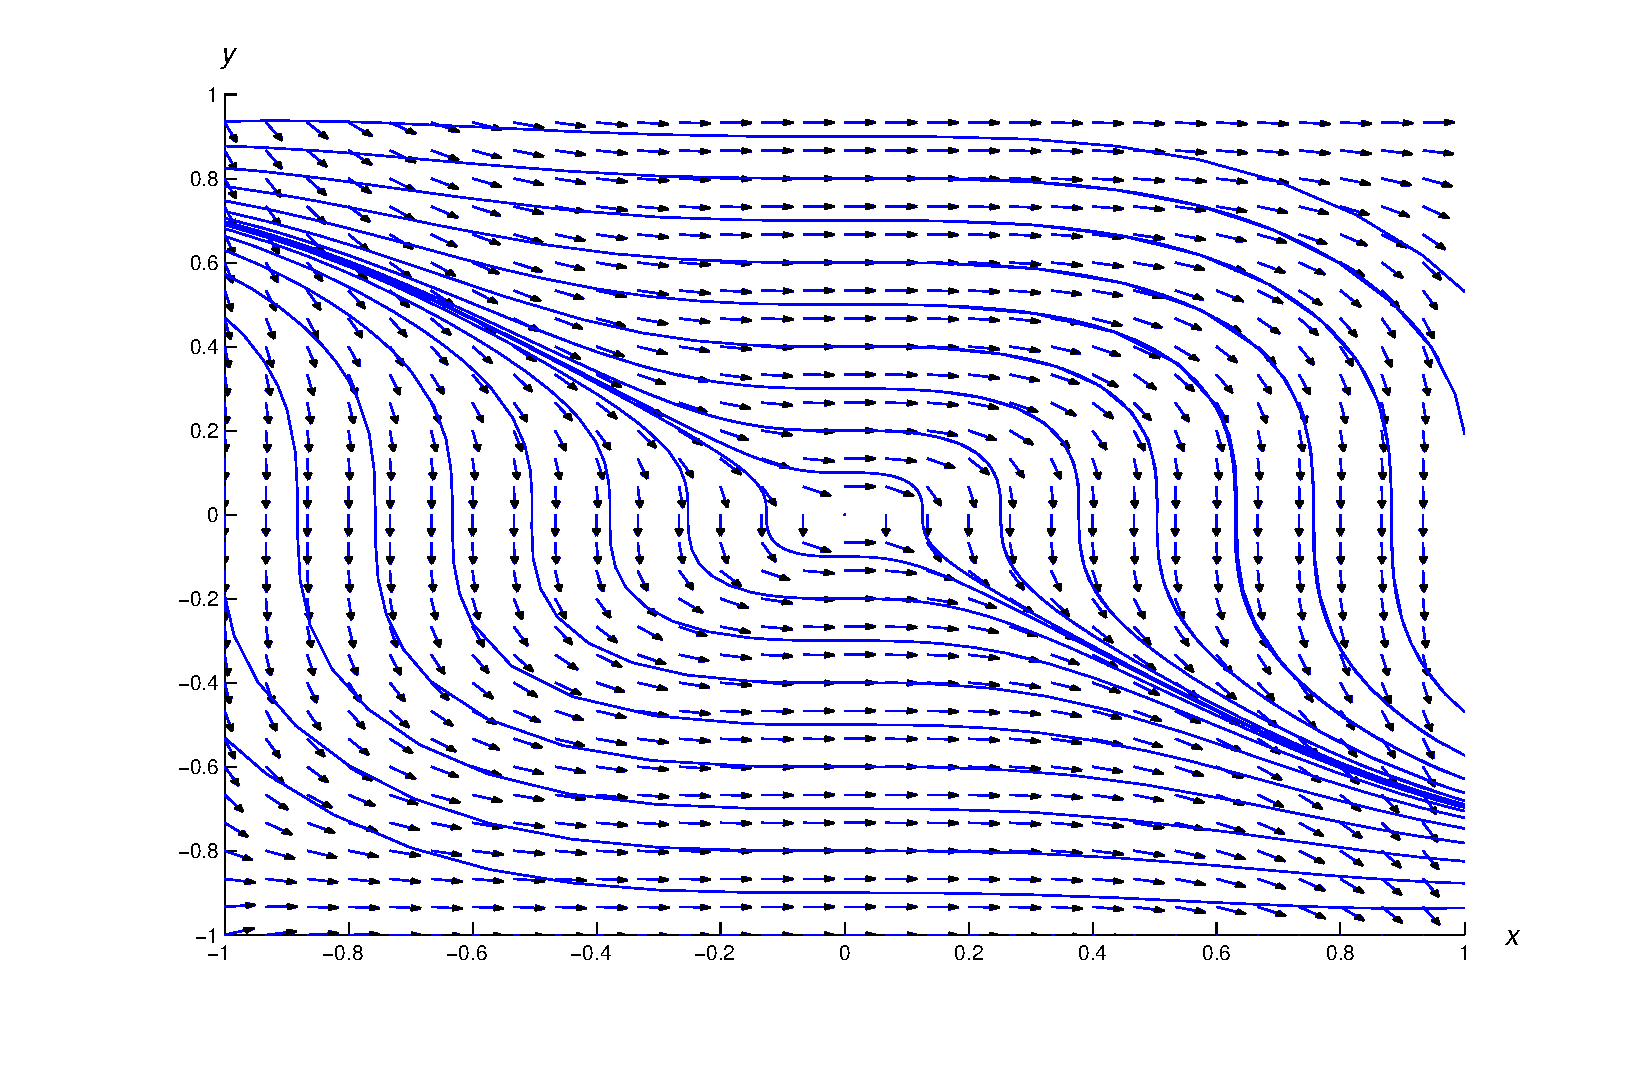
\includegraphics[bb=-78 148 689 643,width=5.67in,height=3.66in,keepaspectratio]{fig020501}
\color{blue}
\caption{A direction field and  integral curves for
$(4x^3y^3+3x^2)\,dx+(3x^4y^2+6y^2)\,dy=0$}
  \label{figure:2.5.1}
\end{figure}

Here's a summary of the procedure used in Method 1 of this
example. You should summarize procedure used in Method~2.

\smallskip
\color{blue}
\centerline{{\bf Procedure For Solving An Exact
Equation}}

\begin{description}
\item{\bf Step 1.} Check that the equation
\begin{equation} \label{eq:2.5.19}
 M(x,y)\,dx+N(x,y)\,dy=0
\end{equation}
satisfies the exactness condition  $M_y=N_x$. If not,
don't go further with this procedure.
\item{\bf Step 2.} Integrate
$$
{\partial F(x,y)\over\partial x}=M(x,y)
$$
with respect to $x$ to obtain
\begin{equation} \label{eq:2.5.20}
F(x,y)=G(x,y)+\phi(y),
\end{equation}
where $G$ is an antiderivative of $M$ with respect to $x$, and $\phi$
is an unknown function of $y$.
\item{\bf Step 3.} Differentiate \eqref{eq:2.5.20} with respect to
$y$  to obtain
$$
{\partial F(x,y)\over\partial y}={\partial G(x,y)\over\partial
y}+\phi'(y).
$$
\item{\bf Step 4.} Equate the right side of this equation to $N$ and solve
for $\phi'$;    thus,
$$
 {\partial G(x,y)\over\partial y}+\phi'(y)=N(x,y),\mbox{\quad  so \quad }
\phi'(y)=N(x,y)-{\partial G(x,y)\over\partial y}.
$$
\item{\bf Step 5.} Integrate $\phi'$ with respect to $y$, taking the
constant of integration to be zero, and substitute the result in
\eqref{eq:2.5.20} to obtain $F(x,y)$.
\item{\bf Step 6.} Set $F(x,y)=c$ to obtain an implicit solution of
\eqref{eq:2.5.19}. If possible, solve for $y$ explicitly as a
function of $x$.
\end{description}
\color{black}

It's a common mistake to omit Step 6. However, it's important to
include this step, since $F$ isn't  itself a solution of
\eqref{eq:2.5.19}.

Many equations can be conveniently solved by either of the two methods
used in Example~\ref{example:2.5.3}. However, sometimes the integration
required in one approach is  more difficult than in the
other. In such cases we choose the approach that requires the easier
integration.

\begin{example}\label{example:2.5.4} \rm
 Solve the equation
\begin{equation}  \label{eq:2.5.21}
(ye^{xy} \tan x+e^{xy} \sec^2x)\,dx+xe^{xy} \tan x\,dy=0.
\end{equation}
\end{example}

\solution We leave it to you to check that
$M_y=N_x$ on any open rectangle  where $\tan x$ and $\sec x$ are
defined. Here we must find a function $F$ such that
\begin{equation} \label{eq:2.5.22}
F_x(x,y)=ye^{xy} \tan x+e^{xy} \sec^2 x
\end{equation}
 and
\begin{equation}  \label{eq:2.5.23}
F_y(x,y)=xe^{xy} \tan x.
\end{equation}
 It's difficult to integrate \eqref{eq:2.5.22} with respect to $x$, but
easy to integrate \eqref{eq:2.5.23} with respect to $y$.  This yields
\begin{equation} \label{eq:2.5.24}
F(x,y)=e^{xy} \tan x+\psi (x).
\end{equation}
Differentiating this with respect to $x$ yields
$$
F_x(x,y)=ye^{xy}\tan x+e^{xy}\sec^2x+\psi'(x).
$$
 Comparing this with \eqref{eq:2.5.22} shows that  $\psi'(x)=0$.
Hence, $\psi$ is  a constant, which we can take to be zero in
\eqref{eq:2.5.24}, and
$$
e^{xy} \tan x=c
$$
is an implicit solution of \eqref{eq:2.5.21}. \bbox

Attempting to apply our procedure to an equation that isn't  exact
will lead to failure in  Step 4, since the function
$$
 N-{\partial G\over\partial y}
$$
won't be independent of $x$ if $M_y\ne N_x$
(Exercise~\ref{exer:2.5.31}), and therefore
can't be the derivative of a function of $y$ alone. Here's an example that
illustrates this.

\begin{example}\label{example:2.5.5}  \rm
 Verify that the equation
\begin{equation} \label{eq:2.5.25}
3x^2y^2\,dx+6x^3y\,dy=0
\end{equation}
is not exact, and show  that the procedure for solving exact equations
  fails when applied to \eqref{eq:2.5.25}.
\end{example}

\solution   Here
$$
M_y(x,y)=6x^2y \mbox{\quad  and \quad } N_x(x,y)=18x^2y,
$$
so \eqref{eq:2.5.25} isn't  exact. Nevertheless,  let's try to find
a function $F$ such that
\begin{equation} \label{eq:2.5.26}
F_x(x,y)=3x^2y^2
\end{equation}
and
\begin{equation} \label{eq:2.5.27}
F_y(x,y)=6x^3y.
\end{equation}
Integrating \eqref{eq:2.5.26} with respect to $x$ yields
$$
F(x,y)=x^3y^2+\phi(y),
$$
and differentiating this with respect to $y$ yields
$$
F_y(x,y)=2x^3y+\phi'(y).
$$
For this equation to be consistent with \eqref{eq:2.5.27},
$$
6x^3y=2x^3y+\phi'(y),
$$
or
$$
\phi'(y)=4x^3y.
$$
This is a contradiction, since $\phi'$  must be independent
of $x$. Therefore the procedure fails.

\exercises
In Exercises~\ref{exer:2.5.1}--\ref{exer:2.5.17} determine which equations
are exact and solve them.

\begin{exerciselist}
\item\label{exer:2.5.1}
$6x^2y^2\,dx+4x^3y\,dy=0$

\item\label{exer:2.5.2}
$(3y\cos x+4xe^x+2x^2e^x)\,dx+(3\sin x+3)\,dy=0$

\item\label{exer:2.5.3}
$14x^2y^3\,dx+21 x^2y^2\,dy=0$

\item\label{exer:2.5.4}
$(2x-2y^2)\,dx+(12y^2-4xy)\,dy=0$

\begin{tabular}[t]{@{}p{168pt}@{}p{168pt}}
 \item\label{exer:2.5.5}$(x+y)^2\,dx+(x+y)^2\,dy=0$&
\item\label{exer:2.5.6}$(4x+7y)\,dx+(3x+4y)\,dy=0$
\end{tabular}

\item\label{exer:2.5.7}
$(-2y^2\sin x+3y^3-2x)\,dx+(4y\cos x+9xy^2)\,dy=0$

\item\label{exer:2.5.8}
$(2x+y)\,dx+(2y+2x)\,dy=0$

\item\label{exer:2.5.9}
$(3x^2+2xy+4y^2)\,dx+(x^2+8xy+18y)\,dy=0$

\item\label{exer:2.5.10}
$(2x^2+8xy+y^2)\,dx+(2x^2+xy^3/3)\,dy=0$

\item\label{exer:2.5.11}
$\dst{\left({1\over x}+2x\right)\,dx+
\left({1\over y}+2y\right)\,dy=0}$

\item\label{exer:2.5.12}
$(y\sin xy+xy^2\cos xy)\,dx+(x\sin xy+xy^2\cos xy)\,dy=0$

\item\label{exer:2.5.13}
$\dst{{x\,dx\over(x^2+y^2)^{3/2}}+{y\,dy
\over(x^2+y^2)^{3/2}}=0}$

\item\label{exer:2.5.14}
$\left(e^x(x^2y^2+2xy^2)+6x\right)\,dx+(2x^2ye^x+2)\,dy=0$

\item\label{exer:2.5.15}
$\left(x^2e^{x^2+y}(2x^2+3)+4x\right)\,dx+(x^3e^{x^2+y}-12y^2)\,dy=0$

\item\label{exer:2.5.16}
$\left(e^{xy}(x^4y+4x^3)+3y\right)\,dx+(x^5e^{xy}+3x)\,dy=0$

\item\label{exer:2.5.17}
$(3x^2\cos xy-x^3y\sin xy+4x)\,dx+(8y-x^4\sin xy)\,dy=0$

\exercisetext{In Exercises~\ref{exer:2.5.18}--\ref{exer:2.5.22} solve
the initial value problem.}

\item\label{exer:2.5.18}
$(4x^3y^2-6x^2y-2x-3)\,dx+(2x^4y-2x^3)\,dy=0,\quad y(1)=3$

\item\label{exer:2.5.19}
$(-4y\cos x+4\sin x\cos x+\sec^2x)\,dx+
(4y-4\sin x)\,dy=0,\quad y(\pi/4)=0$

\item\label{exer:2.5.20}
$(y^3-1)e^x\,dx+3y^2(e^x+1)\,dy=0,\quad y(0)=0$

\item\label{exer:2.5.21}
$(\sin x-y\sin x-2\cos x)\,dx+\cos x\,dy=0,\quad y(0)=1$

\item\label{exer:2.5.22}
$(2x-1)(y-1)\,dx+(x+2)(x-3)\,dy=0,\quad y(1)=-1$

\item\label{exer:2.5.23} \CGex
Solve the exact equation
$$
(7x+4y)\,dx+(4x+3y)\,dy=0.
$$
Plot a direction field and some integral curves for this equation on
the rectangle
$$
\{-1\le x\le1,-1\le y\le1\}.
$$

\item\label{exer:2.5.24} \CGex
Solve the exact equation
$$
e^x(x^4y^2+4x^3y^2+1)\,dx+(2x^4ye^x+2y)\,dy=0.
$$
Plot a direction field and some integral curves for this equation on
the rectangle
$$
\{-2\le x\le2,-1\le y\le1\}.
$$

\item\label{exer:2.5.25} \CGex
Plot a direction field and some integral curves for the exact equation
$$
(x^3y^4+x)\,dx+(x^4y^3+y)\,dy=0
$$
on the rectangle $\{-1\le x\le 1,-1\le y\le1\}$. (See
Exercise~\ref{exer:2.5.37}\part{a}).

\item\label{exer:2.5.26} \CGex
Plot a direction field and some integral curves for the exact equation
$$
(3x^2+2y)\,dx+(2y+2x)\,dy=0
$$
on the rectangle $\{-2\le x\le 2,-2\le y\le2\}$. (See
Exercise~\ref{exer:2.5.37}(b)).

\item\label{exer:2.5.27} \Lex
\begin{alist}
\item % (a)
Solve the exact equation
$$
(x^3y^4+2x)\,dx+(x^4y^3+3y)\,dy=0
\eqno{\rm(A)}
$$
implicitly.
\item % (b)
For what choices of $(x_0,y_0)$ does
Theorem~\ref{thmtype:2.3.1} imply that the initial value problem
$$
(x^3y^4+2x)\,dx+(x^4y^3+3y)\,dy=0,\quad y(x_0)=y_0,
\eqno{\rm(B)}
$$
has a unique solution on an open interval $(a,b)$  that contains $x_0$?
\item % (b)
Plot a direction field and some integral curves for (A)
on a rectangular region centered at the origin. What is the
 interval of validity of the solution of (B)?
\end{alist}

\item\label{exer:2.5.28} \Lex
\begin{alist}
\item % (a)
Solve the exact equation
$$
(x^2+y^2)\,dx+2xy\,dy=0
\eqno{\rm(A)}
$$
implicitly.
\item % (b)
For what choices of $(x_0,y_0)$ does
Theorem~\ref{thmtype:2.3.1} imply that the initial value problem
$$
(x^2+y^2)\,dx+2xy\,dy=0,\quad y(x_0)=y_0,
\eqno{\rm(B)}
$$
has a unique solution $y=y(x)$ on some open interval $(a,b)$
that contains $x_0$?
\item % (c)
Plot a direction field and some integral curves for (A). From
the plot determine,
the  interval $(a,b)$ of \part{b}, the monotonicity
properties (if any) of the solution of (B), and $\lim_{x\to
a+}y(x)$ and $\lim_{x\to b-}y(x)$. \hint{Your answers will
depend upon which quadrant contains $(x_0,y_0)$.}
\end{alist}

\item\label{exer:2.5.29}
Find all functions $M$ such that the  equation is exact.
\begin{alist}
\item %(a)
$M(x,y)\,dx+(x^2-y^2)\,dy=0$
\item %(b)
$M(x,y)\,dx+2xy\sin x\cos y\,dy=0$
\item %(c)
$M(x,y)\,dx+(e^x-e^y\sin x)\,dy=0$
\end{alist}

\item\label{exer:2.5.30}
Find all functions $N$ such that the  equation is exact.
\begin{alist}
\item %(a)
$(x^3y^2+2xy+3y^2)\,dx+N(x,y)\,dy=0$
\item %(b)
$(\ln xy+2y\sin x)\,dx+N(x,y)\,dy=0$
\item %(c)
$(x\sin x+y\sin y)\,dx+N(x,y)\,dy=0$
\end{alist}

\item\label{exer:2.5.31}
Suppose $M$, $N$, and their partial derivatives are continuous on
an open rectangle
$R$, and $G$ is an antiderivative of $M$ with respect to $x$; that is,
$$
{\partial G\over\partial x}=M.
$$
Show that if $M_y\ne N_x$ in $R$ then the function
$$
 N-{\partial  G\over\partial y}
$$
is not independent of $x$.

\item\label{exer:2.5.32}
Prove:  If the equations $M_1\,dx+N_1\,dy=0$ and $M_2\,
dx+N_2\,dy=0$ are exact on an open rectangle $R$,  so is
the equation $$(M_1+M_2)\,dx+(N_1+N_2)\,dy=0.$$

\item\label{exer:2.5.33}
Find conditions on the constants $A$, $B$, $C$, and $D$ such that
the equation
$$
(Ax+By)\,dx+(Cx+Dy)\,dy=0
$$
is exact.

\item\label{exer:2.5.34}
Find conditions on the constants $A$, $B$, $C$, $D$, $E$, and
$F$ such that the equation
$$
(Ax^2+Bxy+Cy^2)\,dx+(Dx^2+Exy+Fy^2)\,dy=0
$$
is exact.

\item\label{exer:2.5.35}
Suppose $M$ and $N$ are continuous and have continuous partial
derivatives $M_y$ and $N_x$ that satisfy the exactness condition
$M_y=N_x$ on an open rectangle $R$.
  Show that if $(x,y)$ is in $R$ and
$$
F(x,y)=\int^x_{x_0}M(s,y_0)\,ds+\int^y_{y_0}N(x,t)\,dt,
$$
then $F_x=M$ and $F_y=N$.

\item\label{exer:2.5.36}
Under the assumptions of Exercise~\ref{exer:2.5.35}, show that
$$
F(x,y)=\int^y_{y_0}N(x_0,s)\,ds+\int^x_{x_0}M(t,y)\,dt.
$$

\item\label{exer:2.5.37}
Use the method suggested by Exercise~\ref{exer:2.5.35}, with
$(x_0,y_0)=(0,0)$, to solve the these exact equations:
\begin{alist}
\item %(a)
$(x^3y^4+x)\,dx+(x^4y^3+y)\,dy=0$
\item %(b)
$(x^2+y^2)\,dx+2xy\,dy=0$
\item %(c)
$(3x^2+2y)\,dx+(2y+2x)\,dy=0$
\end{alist}

\item\label{exer:2.5.38}
Solve the initial value problem
$$
y'+{2\over x}y=-{2xy\over x^2+2x^2y+1},\quad y(1)=-2.
$$

\item\label{exer:2.5.39}
Solve the initial value problem
$$
y'-{3\over x}y={2x^4(4x^3-3y)\over3x^5+3x^3+2y},\quad y(1)=1.
$$

\item\label{exer:2.5.40}
Solve the initial value problem
$$
y'+2xy=-e^{-x^2}\left({3x+2ye^{x^2}\over2x+3ye^{x^2}}\right),\quad
y(0)=-1.
$$

\item\label{exer:2.5.41}
Rewrite the separable equation
$$
h(y)y'=g(x)
\eqno{\rm (A)}
$$
as an exact equation
$$
M(x,y)\,dx+N(x,y)\,dy=0.
\eqno{\rm (B)}
$$
Show that applying the method of this section  to
(B) yields the same solutions that would be
obtained by applying the method of separation of variables
to~(A)

\item\label{exer:2.5.42}
Suppose  all second partial derivatives of $M=M(x,y)$ and $N=N(x,y)$
are continuous and $M\,dx+N\,dy=0$ and $-N\,dx+M\,dy=0$ are
exact on an open rectangle  $R$.  Show that
$M_{xx}+M_{yy}=N_{xx}+N_{yy}=0$ on
$R$.

\item\label{exer:2.5.43} Suppose all second partial derivatives of
$F=F(x,y)$ are continuous and $F_{xx}+F_{yy}=0$ on an open rectangle
$R$. (A function with these properties is said to be {\color{blue}\it harmonic\/};
see also Exercise~\ref{exer:2.5.42}.) Show that $-F_y\,dx+F_x\,dy=0$ is
exact on $R$, and
therefore there's a function $G$ such that
$G_x=-F_y$ and $G_y=F_x$ in $R$. (A function $G$ with this property is
said to be a {\color{blue}\it harmonic conjugate\/} of $F$.)

\item\label{exer:2.5.44}
Verify that the following functions are harmonic, and find all their
harmonic conjugates.  (See Exercise~\ref{exer:2.5.43}.)

\begin{tabular}[t]{@{}p{112pt}@{}p{112pt}p{112pt}}
{\bf (a)}\   $x^2-y^2$
& {\bf (b)}\   $e^x\cos y$
& {\bf (c)}\   $x^3-3xy^2$\\
{\bf (d)}\   $\cos x\cosh y$
& {\bf (e)}\   $\sin x\cosh y$ &
\end{tabular}

\end{exerciselist}


\section{Integrating Factors}

\noindent
In  Section~2.5 we saw that if $M$, $N$, $M_y$ and $N_x$ are
continuous and $M_y=N_x$ on an open rectangle $R$ then
\begin{equation} \label{eq:2.6.1}
M(x,y)\,dx+N(x,y)\,dy=0
\end{equation}
is exact on $R$. Sometimes an equation that isn't  exact can be made
exact by multiplying it by an appropriate function. For example,
\begin{equation}\label{eq:2.6.2}
(3x+2y^2)\,dx+2xy\,dy=0
\end{equation}
is  not exact, since
$M_y(x,y)=4y\ne  N_x(x,y)=2y$ in \eqref{eq:2.6.2}.
 However, multiplying \eqref{eq:2.6.2}  by $x$ yields
\begin{equation}\label{eq:2.6.3}
(3x^2+2xy^2)\,dx+2x^2y\,dy=0,
\end{equation}
which is exact, since
$M_y(x,y)=N_x(x,y)=4xy$ in \eqref{eq:2.6.3}.
Solving \eqref{eq:2.6.3} by the procedure given in  Section~2.5
 yields the implicit solution
$$
x^3+x^2y^2=c.
$$

A function $\mu=\mu(x,y)$ is  an {\color{blue}\it integrating factor} for
\eqref{eq:2.6.1}  if
\begin{equation}\label{eq:2.6.4}
 \mu(x,y)M (x,y)\,dx+\mu(x,y)N (x,y)\,dy=0
 \end{equation}
 is exact. If we know an integrating
factor $\mu$ for \eqref{eq:2.6.1}, we can solve the exact equation
\eqref{eq:2.6.4} by the method of Section~2.5. It would be
nice
if we could say that \eqref{eq:2.6.1} and \eqref{eq:2.6.4} always have the
same solutions, but this isn't so. For example, a solution
$y=y(x)$ of \eqref{eq:2.6.4} such that $\mu(x,y(x))=0$ on some interval
$a<x<b$ could fail to be a solution of \eqref{eq:2.6.1}
(Exercise~\ref{exer:2.6.1}), while
\eqref{eq:2.6.1} may have a solution $y=y(x)$ such that $\mu(x,y(x)) $
isn't even defined (Exercise~\ref{exer:2.6.2}). Similar comments
apply if $y$ is the independent variable and $x$ is the dependent
variable  in \eqref{eq:2.6.1} and \eqref{eq:2.6.4}.  However, if $\mu(x,y)$
is defined and nonzero for all $(x,y)$,  \eqref{eq:2.6.1}  and
\eqref{eq:2.6.4} are equivalent; that is, they have the same solutions.

\boxit{Finding Integrating Factors}

\noindent
By applying Theorem~\ref{thmtype:2.5.2} (with $M$ and $N$ replaced by $\mu M$
and $\mu N$), we see that \eqref{eq:2.6.4} is exact on an open rectangle
$R$ if $\mu M$, $\mu N$, $(\mu M)_y$, and $(\mu N)_x$ are continuous
and
$$
{\partial\over\partial y}(\mu M)={\partial\over\partial x}
(\mu N) \mbox{\quad or, equivalently, \quad}
\mu_yM+\mu M_y=\mu_xN+\mu N_x
$$
on $R$. It's better to rewrite the last equation as
\begin{equation} \label{eq:2.6.5}
\mu(M_y-N_x)=\mu_xN-\mu_yM,
\end{equation}
which  reduces to  the known result for exact equations;
that is, if $M_y=N_x$ then \eqref{eq:2.6.5} holds with $\mu=1$, so
\eqref{eq:2.6.1} is exact.

You may think  \eqref{eq:2.6.5} is of little value, since it involves
{\color{blue}\it partial\/} derivatives of the unknown integrating factor $\mu$,
and we haven't studied methods for solving such equations. However,
we'll now show that \eqref{eq:2.6.5} is useful if we restrict our search
to integrating factors that are products of a function of
$x$ and a function of $y$; that is,
$\mu(x,y)=P(x)Q(y)$.
We're not saying that {\color{blue}\it every\/} equation
 $M\,dx+N\,dy=0$ has an integrating factor of this
form;   rather, we're saying that {\color{blue}\it some\/} equations have
such integrating
factors. We'll now develop a way to determine whether a given
equation has such an integrating factor, and a method for finding the
integrating factor in this case.

If $\mu(x,y)=P(x)Q(y)$, then $\mu_x(x,y)=P'(x)Q(y)$ and
$\mu_y(x,y)=P(x)Q'(y)$, so \eqref{eq:2.6.5} becomes
\begin{equation} \label{eq:2.6.6}
P(x)Q(y)(M_y-N_x)=P'(x)Q(y)N-P(x)Q'(y)M,
\end{equation}
or, after dividing through by $P(x)Q(y)$,
\begin{equation} \label{eq:2.6.7}
M_y-N_x={P'(x)\over P(x)}N-{Q'(y)\over Q(y)}M.
\end{equation}
Now let
$$
p(x)={P'(x)\over P(x)} \mbox{\quad and \quad} q(y)={Q'(y)\over Q(y)},
$$
so \eqref{eq:2.6.7} becomes
\begin{equation} \label{eq:2.6.8}
M_y-N_x=p(x)N-q(y)M.
\end{equation}

We obtained \eqref{eq:2.6.8} by {\color{blue}\it assuming\/} that $M\,dx+N\,dy=0$ has
an integrating factor $\mu(x,y)=P(x)Q(y)$. However, we can
now view \eqref{eq:2.6.7} differently: If there are functions $p=p(x)$
and $q=q(y)$  that satisfy \eqref{eq:2.6.8} and we define
\begin{equation} \label{eq:2.6.9}
P(x)=\pm e^{\int p(x)\,dx}\mbox{\quad and \quad}
Q(y)=\pm e^{\int q(y)\,dy},
\end{equation}
then reversing the steps that led from \eqref{eq:2.6.6} to
\eqref{eq:2.6.8} shows that $\mu(x,y)=P(x)Q(y)$ is an integrating factor
for $M\,dx+N\,dy=0$. In using this result, we take the constants of
integration in \eqref{eq:2.6.9} to be zero and choose the signs
conveniently so the integrating factor has the simplest form.

There's no simple general method for ascertaining
whether functions $p=p(x)$ and $q=q(y)$ satisfying \eqref{eq:2.6.8}
exist. However, the next theorem gives simple sufficient
conditions for the given equation to have an integrating factor that
depends on only one of the independent variables $x$ and $y$, and for
finding an integrating factor in this case.

\begin{theorem}\color{blue}\label{thmtype:2.6.1}
Let $M,$ $N,$ $M_y,$ and $N_x$ be continuous on an open rectangle $R.$
Then$:$
\begin{alist}
\item % (a)
 If $(M_y-N_x)/N$ is independent
of $y$ on $R$ and  we define
$$
p(x)={M_y-N_x\over N}
$$
 then
\begin{equation}\label{eq:2.6.10}
\mu(x)=\pm e^{\int p(x)\,dx}
\end{equation}
is an integrating factor for
\begin{equation}\label{eq:2.6.11}
M(x,y)\,dx+N(x,y)\,dy=0
\end{equation}
on $R.$
\item % (b)
If $(N_x-M_y)/M$ is independent of $x$ on
$R$ and we define
$$
q(y)={N_x-M_y\over M},
$$
then
\begin{equation}\label{eq:2.6.12}
\mu(y)=\pm e^{\int q(y)\,dy}
\end{equation}
 is an integrating factor for \eqref{eq:2.6.11} on $R.$
\end{alist}
\end{theorem}

\medskip

\proof (a)
If $(M_y-N_x)/N$ is independent of $y$, then \eqref{eq:2.6.8}
 holds with $p=(M_y-N_x)/N$ and $q\equiv0$. Therefore
 $$
P(x)=\pm e^{\int p(x)\,dx}\mbox{\quad and\quad}Q(y)=\pm e^{\int
q(y)\,dy}=\pm e^0=\pm1,
 $$
so \eqref{eq:2.6.10} is an integrating factor for \eqref{eq:2.6.11} on $R$.

(b) If $(N_x-M_y)/M$ is independent of $x$ then eqref{eq:2.6.8} holds
with $p\equiv0$ and $q=(N_x-M_y)/M$, and a similar argument shows that
\eqref{eq:2.6.12} is an integrating factor for \eqref{eq:2.6.11} on $R$.\bbox

The next two examples show how to apply
Theorem~\ref{thmtype:2.6.1}.

\begin{example}\label{example:2.6.1}
\rm  Find an integrating factor for the equation
\begin{equation}\label{eq:2.6.13}
(2xy^3-2x^3y^3-4xy^2+2x)\,dx+(3x^2y^2+4y)\,dy=0
\end{equation}
and solve the equation.
\end{example}

\solution In \eqref{eq:2.6.13}
$$
M=2xy^3-2x^3y^3-4xy^2+2x,\ N=3x^2y^2+4y,
$$
and
$$
M_y-N_x=(6xy^2-6x^3y^2-8xy)-6xy^2=-6x^3y^2-8xy,
$$
so \eqref{eq:2.6.13}  isn't  exact. However,
$$
{M_y-N_x\over N}=-{6x^3y^2+8xy\over
3x^2y^2+4y}=-2x
$$
is independent of $y$, so Theorem~\ref{thmtype:2.6.1}\part{a} applies
with
$p(x)=-2x$. Since
$$
\int p (x)\,dx=-\int 2x\,dx=-x^2,
$$
 $\mu(x)=e^{-x^2}$ is an
integrating factor.  Multiplying \eqref{eq:2.6.13} by $\mu$ yields the
exact equation
\begin{equation}\label{eq:2.6.14}
e^{-x^2}(2xy^3-2x^3y^3-4xy^2+2x)\,dx+
 e^{-x^2}(3x^2y^2+4y)\,dy=0.
\end{equation}

To solve this equation, we must find a
function $F$ such that
\begin{equation}\label{eq:2.6.15}
F_x(x,y)=e^{-x^2}(2xy^3-2x^3y^3-4xy^2+2x)
\end{equation}
 and
\begin{equation}\label{eq:2.6.16}
F_y(x,y)=e^{-x^2}(3x^2y^2+4y).
\end{equation}
 Integrating \eqref{eq:2.6.16} with respect to $y$ yields
\begin{equation}\label{eq:2.6.17}
F(x,y)=e^{-x^2}(x^2y^3+2y^2)+\psi(x).
\end{equation}
 Differentiating this with respect to $x$ yields
$$
F_x(x,y)=e^{-x^2}(2xy^3-2x^3y^3-4xy^2)+\psi'(x).
$$
Comparing this with \eqref{eq:2.6.15} shows that $\psi'(x)=
2xe^{-x^2}$;  therefore, we can let $\psi(x)=-e^{-x^2}$ in
\eqref{eq:2.6.17} and conclude that
$$
e^{-x^2}\left(y^2(x^2y+2)-1\right)=c
$$
is an implicit solution of \eqref{eq:2.6.14}. It is also an implicit solution
of \eqref{eq:2.6.13}.

Figure~\ref{figure:2.6.1}  shows a  direction field and some integral curves
for \eqref{eq:2.6.13}

  \begin{figure}[tbp]
  \centering
  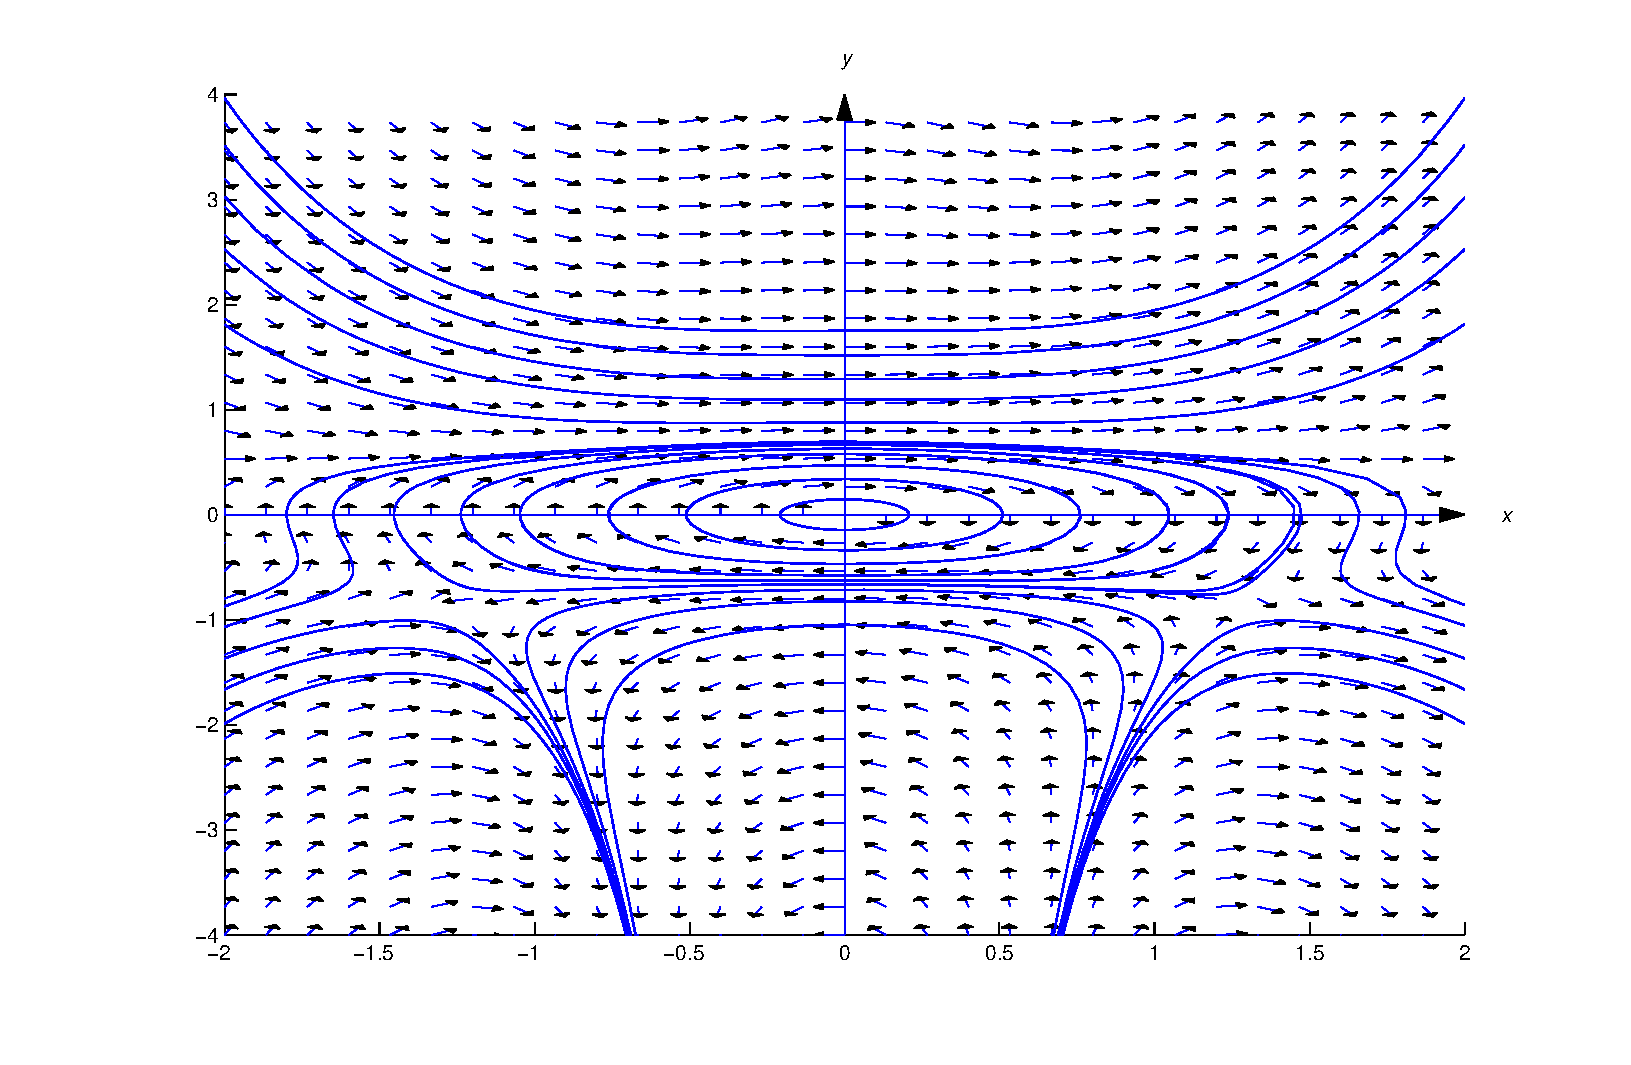
\includegraphics[bb=-78 148 689 643,width=5.67in,height=3.66in,keepaspectratio]{fig020601}
\color{blue}
\caption{A direction field and  integral curves for
$(2xy^3-2x^3y^3-4xy^2+2x)\,dx+(3x^2y^2+4y)\,dy=0$}
  \label{figure:2.6.1}
\end{figure}

\begin{example}\label{example:2.6.2}
\rm  Find an integrating factor for
\begin{equation}\label{eq:2.6.18}
2xy^3\,dx+(3x^2y^2+x^2y^3+1)\,dy=0
\end{equation}
and solve the equation.
\end{example}

\solution In \eqref{eq:2.6.18},
$$
M=2xy^3,\quad N=3x^2y^2+x^2y^3+1,
$$
and
$$
M_y-N_x=6xy^2-(6xy^2+2xy^3)=-2xy^3,
$$
so \eqref{eq:2.6.18} isn't  exact.  Moreover,
$$
{M_y-N_x\over N}=-{2xy^3\over 3x^2y^2+x^2y^2+1}
$$
is not independent of $y$, so Theorem~\ref{thmtype:2.6.1}(a) does not
apply. However,   Theorem~\ref{thmtype:2.6.1}(b) does apply, since
$$
{N_x-M_y\over M}={2xy^3\over 2xy^3}=1
$$
is independent of $x$, so we can take $q(y)=1$.
 Since
$$
\int q(y)\,dy=\int\,dy=y,
$$
  $\mu(y)=e^y$ is
an integrating factor. Multiplying \eqref{eq:2.6.18} by $\mu$ yields the
exact equation
\begin{equation}\label{eq:2.6.19}
2xy^3e^y\,dx+(3x^2y^2+x^2y^3+1)e^y\,dy=0.
\end{equation}
To solve this equation, we must find a
function $F$ such that
\begin{equation}\label{eq:2.6.20}
F_x(x,y)=2xy^3e^y
\end{equation}
 and
\begin{equation}\label{eq:2.6.21}
F_y(x,y)=(3x^2y^2+x^2y^3+1)e^y.
\end{equation}
 Integrating \eqref{eq:2.6.20} with respect to $x$ yields
\begin{equation}\label{eq:2.6.22}
F(x,y)=x^2y^3e^y+\phi(y).
\end{equation}
Differentiating this with respect to $y$ yields
$$
F_y=(3x^2y^2+x^2y^3)e^y+\phi'(y),
$$
and comparing this with \eqref{eq:2.6.21} shows that $\phi'(y)=e^y$.
 Therefore we set $\phi(y)=e^y$ in \eqref{eq:2.6.22} and conclude
that
$$
(x^2y^3+1)e^y=c
$$
is an implicit solution of \eqref{eq:2.6.19}.
It is also an implicit solution
 of \eqref{eq:2.6.18}. Figure~\ref{figure:2.6.2} shows a direction
field and some integral curves for \eqref{eq:2.6.18}.\bbox

           \begin{figure}[H]
  \centering
  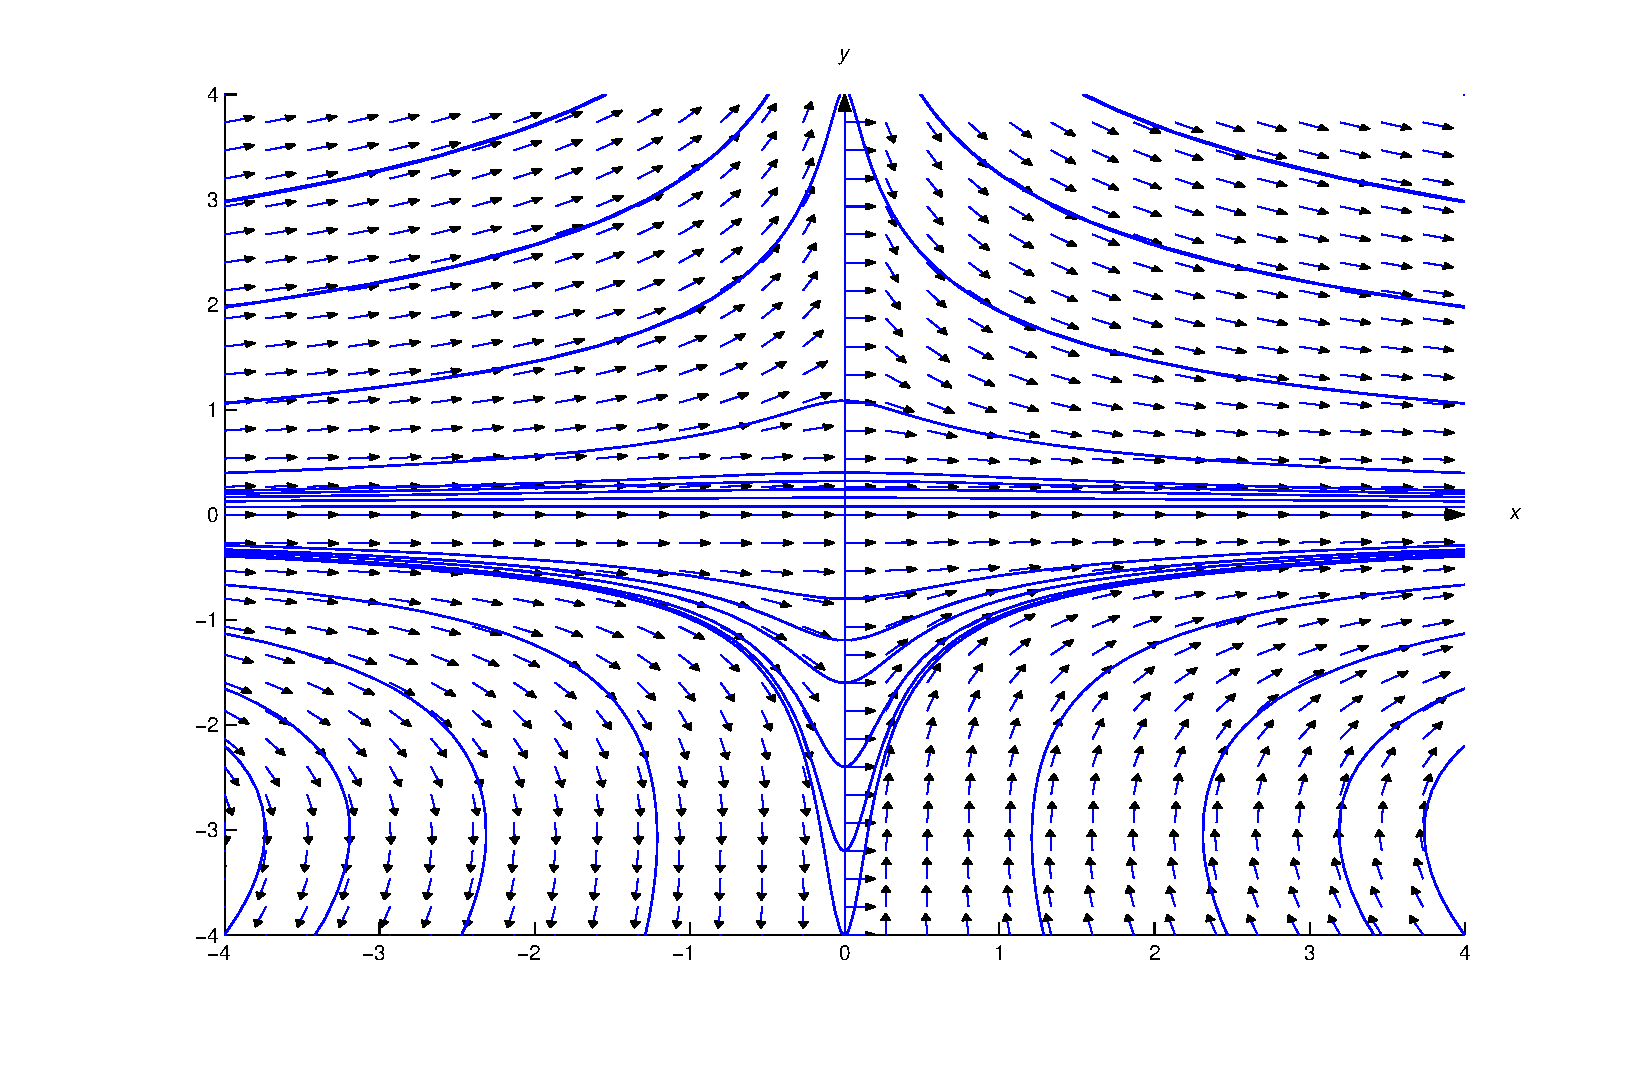
\includegraphics[bb=-78 148 689 643,width=5.67in,height=3.66in,keepaspectratio]{fig020602}
\color{blue}
\caption{
A direction field and integral curves for
$2xy^3e^y\,dx+(3x^2y^2+x^2y^3+1)e^y\,dy=0$}
  \label{figure:2.6.2}
\end{figure}

Theorem~\ref{thmtype:2.6.1} does not apply in the next example,
but the more general argument that led to Theorem~\ref{thmtype:2.6.1}
provides an integrating factor.

\begin{example}\label{example:2.6.3} \rm Find an integrating factor for
\begin{equation}\label{eq:2.6.23}
(3xy+6y^2)\,dx+(2x^2+9xy)\,dy=0
\end{equation} and solve the equation.
 \end{example}

\solution In \eqref{eq:2.6.23}
 $$
 M=3xy+6y^2,\ N=2x^2+9xy,
 $$
and
 $$
M_y-N_x=(3x+12y)-(4x+9y)=-x+3y.
$$
 Therefore
 $$ {M_y-N_x\over
M}={-x+3y\over 3xy+6y^2} \mbox{\quad and \quad} {N_x-M_y\over
N}={x-3y\over 2x^2+9xy},
 $$
so Theorem~\ref{thmtype:2.6.1} does not apply.
Following the more general argument that led to
Theorem~\ref{thmtype:2.6.1}, we look for functions $p=p(x)$ and $q=q(y)$
such that
$$
M_y-N_x=p(x)N-q(y)M;
 $$ that is,
$$
-x+3y=p(x)(2x^2+9xy)-q(y)(3xy+6y^2).
$$
Since the left side contains
only first degree terms in $x$ and $y$, we rewrite this equation as
$$
xp(x)(2x+9y)-yq(y)(3x+6y)=-x+3y.
 $$
 This will be an identity if
\begin{equation}\label{eq:2.6.24}
 xp(x)=A\mbox{\quad and\quad} yq(y)=B,
\end{equation}
 where $A$ and $B$ are constants such that
$$
-x+3y=A(2x+9y)-B(3x+6y),
 $$
 or, equivalently,
$$
-x+3y=(2A-3B)x+(9A-6B)y.
$$
Equating the coefficients of $x$ and $y$
on both sides shows that the last equation holds for all $(x,y)$ if
\begin{eqnarray*} 2A-3B &=&-1 \\ 9A-6B &=&\phantom{-}3,
\end{eqnarray*}
 which has the solution $A=1$, $B=1$. Therefore
\eqref{eq:2.6.24} implies that
 $$ p(x)={1\over x}\mbox{\quad and \quad}
q(y)={1\over y}.
$$
Since
 $$ \int p(x)\,dx=\ln|x|\mbox{\quad
and\quad}\int q(y)\,dy=\ln|y|,
$$
 we can let $P(x)=x$ and $Q(y)=y$;
hence, $\mu(x,y)=xy$ is an integrating factor. Multiplying
\eqref{eq:2.6.23} by $\mu$ yields the exact equation
$$
(3x^2y^2+6xy^3)\,dx+(2x^3y+9x^2y^2)\,dy=0.
 $$
 We leave it to you to
use the method of Section~2.5 to show that this equation has the
implicit solution
\begin{equation}
 \label{eq:2.6.25} x^3y^2+3x^2y^3=c.
\end{equation}
This is also an implicit solution of \eqref{eq:2.6.23}.
Since $x\equiv0$ and $y\equiv0$ satisfy \eqref{eq:2.6.25}, you should
check to see that $x\equiv0$ and $y\equiv0$ are also solutions of
\eqref{eq:2.6.23}. (Why is it necessary to check this?)

Figure~\ref{figure:2.6.3} shows a direction field and integral curves for
\eqref{eq:2.6.23}.

See Exercise~\ref{exer:2.6.28} for a general discussion of equations like
\eqref{eq:2.6.23}.

        \begin{figure}[tbp]
  \centering
  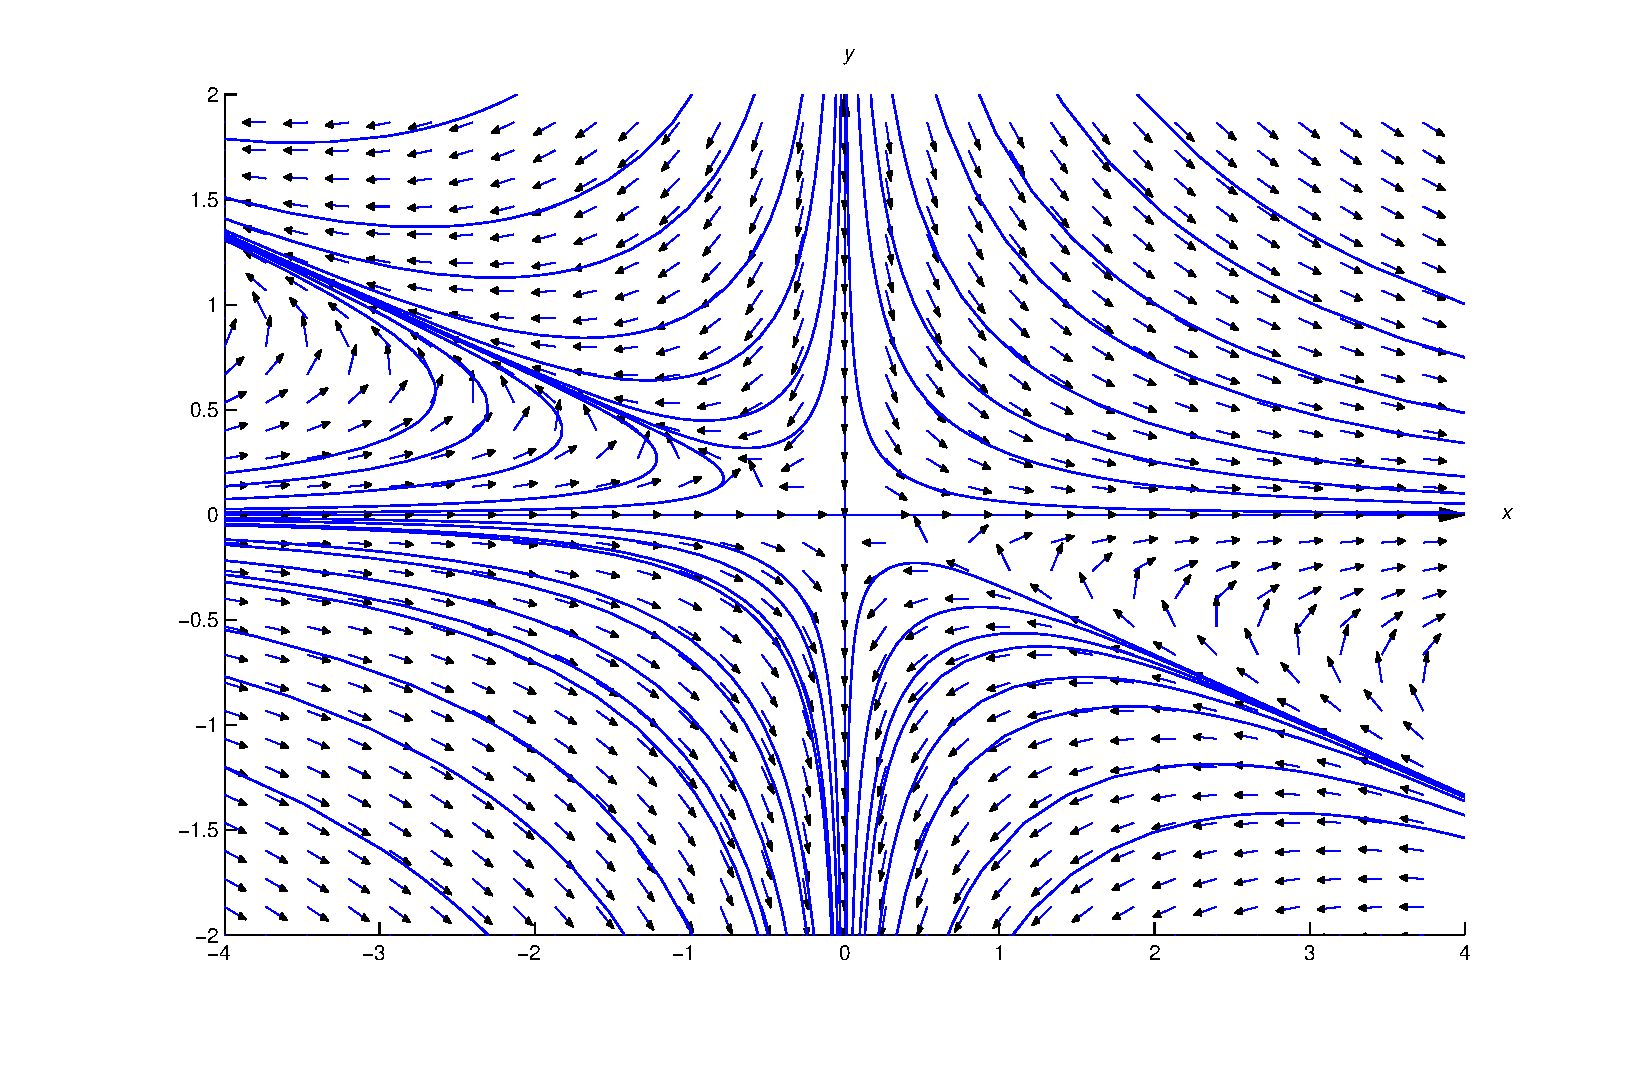
\includegraphics[bb=-78 148 689 643,width=5.67in,height=3.66in,keepaspectratio]{fig020603}
\color{blue}
\caption{
A direction field and integral curves for
$(3xy+6y^2)\,dx+(2x^2+9xy)\,dy=0$}
  \label{figure:2.6.3}
\end{figure}

\begin{example}\label{example:2.6.4}
\rm  The separable  equation
\begin{equation}\label{eq:2.6.26}
-y\,dx+(x+x^6)\,dy=0
\end{equation}
can be converted to the exact equation
\begin{equation} \label{eq:2.6.27}
-{dx\over x+x^6}+{dy\over y}=0
\end{equation}
by multiplying through
by the  integrating factor
$$
\mu(x,y)={1\over y(x+x^6)}.
$$
However, to solve \eqref{eq:2.6.27} by the method of Section~2.5
we would have to evaluate the nasty integral
$$
\int {dx\over x+x^6}.
$$
Instead, we solve \eqref{eq:2.6.26} explicitly for $y$ by finding  an
integrating factor of the form
$\mu(x,y)=x^ay^b$.
\end{example}

\begin{figure}[H]
  \centering
  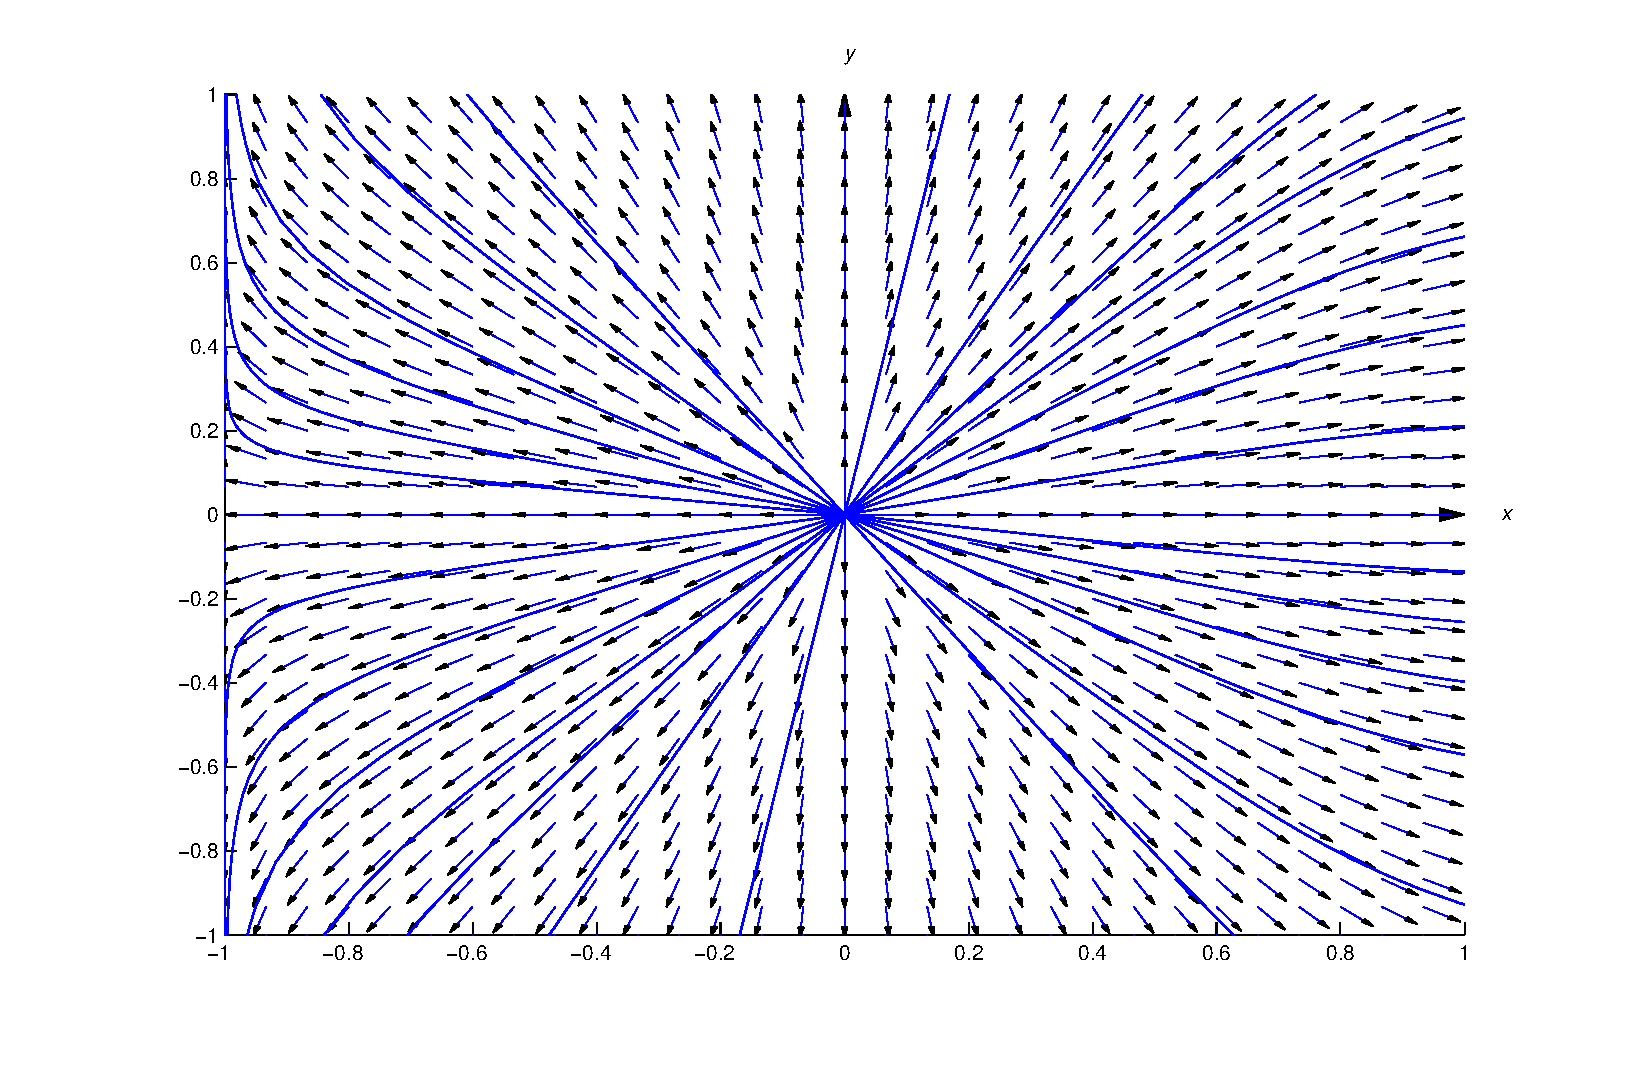
\includegraphics[bb=-78 148 689 643,width=5.67in,height=3.66in,keepaspectratio]{fig020604}
\color{blue}
\caption{A direction field and integral curves for $-y\,dx+(x+x^6)\,dy=0$}
  \label{figure:2.6.4}
\end{figure}

\solution
In \eqref{eq:2.6.26}
$$
M=-y,\ N=x+x^6,
$$
and
$$
M_y-N_x=-1-(1+6x^5)=-2-6x^5.
$$
We  look for functions
$p=p(x)$ and $q=q(y)$ such that
$$
M_y-N_x=p(x)N-q(y)M;
$$
that is,
\begin{equation}\label{eq:2.6.28}
-2-6x^5=p(x)(x+x^6)+q(y)y.
\end{equation}
The right side will contain the term $-6x^5$ if $p(x)=-6/x$.   Then
\eqref{eq:2.6.28} becomes
$$
-2-6x^5=-6-6x^5+q(y)y,
$$
so  $q(y)=4/y$.  Since
$$
\int p(x)\,dx=-\int{6\over x}\,dx=-6\ln|x|=\ln{1\over x^6},
$$
 and
$$
\int q(y)\,dy=\int{4\over y}\,dy=4\ln
|y|=\ln{y^4},
$$
we can take $P(x)=x^{-6}$ and $Q(y)=y^4$,
which yields the integrating factor $\mu(x,y)=x^{-6}y^4$.
Multiplying \eqref{eq:2.6.26} by  $\mu$ yields the exact equation
$$
-{y^5\over x^6}\,dx+\left({y^4\over x^5}+y^4\right)
\,dy=0.
$$
 We leave it to you to use the method of the Section~2.5
to show that this equation has the implicit solution $$
\left({y\over x}\right)^5+y^5=k.
$$
 Solving for $y$ yields
$$
y=k^{1/5}x(1+x^5)^{-1/5},
$$
which we rewrite as
$$
y=cx(1+x^5)^{-1/5}
$$
by renaming the arbitrary constant.
 This is also a solution of \eqref{eq:2.6.26}.

Figure~\ref{figure:2.6.4} shows a direction field and some integral curves
 for \eqref{eq:2.6.26}.

 \exercises
\begin{exerciselist}

\item\label{exer:2.6.1}
\begin{alist}
\item % (a)
Verify that $\mu(x,y)=y$ is an integrating factor for
$$
y\,dx+\left(2x+{1\over y}\right)\,dy=0
\eqno{\rm (A)}
$$
on any open rectangle that does not intersect  the $x$ axis
or, equivalently,  that
$$
y^2\,dx+(2xy+1)\,dy=0
\eqno{\rm (B)}
$$
is exact on any such rectangle.
\item % (b)
Verify that $y\equiv0$  is a solution of  (B),
but not of  (A).
\item % (b)
Show that
$$
y(xy+1)=c
\eqno{\rm (C)}
$$
is an implicit solution of (B), and explain why
every differentiable function $y=y(x)$ other than $y\equiv0$
that satisfies  (C)
 is also a solution of~(A).
\end{alist}

\item\label{exer:2.6.2}
\begin{alist}
\item % (a)
Verify that $\mu(x,y)=1/(x-y)^2$ is an integrating factor for
$$
-y^2\,dx+x^2\,dy=0
\eqno{\rm (A)}
$$
on any open rectangle  that does not intersect the line $y=x$
or, equivalently, that
$$
-{y^2\over(x-y)^2}\,dx+{x^2\over(x-y)^2}\,dy=0
\eqno{\rm (B)}
$$
is exact on any such rectangle.
\item % (b)
Use Theorem~\ref{thmtype:2.2.1} to show that
$$
{xy\over(x-y)}=c
\eqno{\rm (C)}
$$
is an implicit solution of (B), and explain why
it's also an implicit solution of (A)
\item % (b)
Verify that $y=x$  is a solution of  (A),
even though it can't be obtained from  (C).
\end{alist}

\exercisetext{In Exercises~\ref{exer:2.6.3}--\ref{exer:2.6.16} find an
integrating factor;
that is a function of only one variable, and solve the given equation.}

\begin{tabular}[t]{@{}p{168pt}@{}p{168pt}}
\item\label{exer:2.6.3} $y\,dx-x\,dy=0$ &
\item\label{exer:2.6.4} \vspace*{7.5pt} $3x^2y\,dx+2x^3\,dy=0$
\end{tabular}

\begin{tabular}[t]{@{}p{168pt}@{}p{168pt}}
\item\label{exer:2.6.5} $2y^3\,dx+3y^2\,dy=0$&
\item\label{exer:2.6.6} $(5xy+2y+5)\,dx+2x\,dy=0$
\end{tabular}

\item\label{exer:2.6.7} $(xy+x+2y+1)\,dx+(x+1)\,dy=0$

\item\label{exer:2.6.8} $(27xy^2+8y^3)\,dx+(18x^2y+12xy^2)\,dy=0$

\item\label{exer:2.6.9} $(6xy^2+2y)\,dx+(12x^2y+6x+3)\,dy=0$

\item\label{exer:2.6.10} $y^2\,dx+\dst{\left(xy^2+3xy+{1\over
y}\right)\,dy=0}$

\item\label{exer:2.6.11} $(12x^3y+24x^2y^2)\,dx+(9x^4+32x^3y+4y)\,dy=0$

\item\label{exer:2.6.12} $(x^2y+4xy+2y)\,dx+(x^2+x)\,dy=0$

\item\label{exer:2.6.13} $-y\,dx+(x^4-x)\,dy=0$

\item\label{exer:2.6.14} $\cos x\cos y\,dx
+(\sin x\cos y-\sin x\sin y+y)\,dy=0$

\item\label{exer:2.6.15} $(2xy+y^2)\,dx+(2xy+x^2-2x^2y^2-2xy^3)\,dy=0$

\item\label{exer:2.6.16} $y\sin y\,dx+x(\sin y-y\cos y)\,dy=0$

\exercisetext{In Exercises~\ref{exer:2.6.17}--\ref{exer:2.6.23} find an
integrating
factor of the form $\mu(x,y)=P(x)Q(y)$ and solve the given equation.}

\item\label{exer:2.6.17}
$y(1+5\ln|x|)\,dx+4x\ln|x|\,dy=0$

 \item\label{exer:2.6.18}
 $(\alpha y+ \gamma xy)\,dx+(\beta x+ \delta xy)\,dy=0$

\item\label{exer:2.6.19}
$(3x^2y^3-y^2+y)\,dx+(-xy+2x)\,dy=0$

\item\label{exer:2.6.20} $2y\,dx+ 3(x^2+x^2y^3)\,dy=0$

\item\label{exer:2.6.21}
$(a\cos xy-y\sin xy)\,dx+(b\cos xy-x\sin xy)\,
dy=0$

\item\label{exer:2.6.22}
$x^4y^4\,dx+x^5y^3\,dy=0$

\item\label{exer:2.6.23}
$y(x\cos x+2\sin x)\,dx+x(y+1)\sin x\,dy=0$

\exercisetext{In Exercises~\ref{exer:2.6.24}--\ref{exer:2.6.27} find an
integrating factor
and solve the  equation. Plot a direction field and some
integral curves for the equation in the indicated rectangular region.}

\item\label{exer:2.6.24} \CGex
 $(x^4y^3+y)\,dx+(x^5y^2-x)\,dy=0;   \quad \{-1\le x\le1,-1\le y\le1\}$

\item\label{exer:2.6.25} \CGex
$(3xy+2y^2+y)\,dx+(x^2+2xy+x+2y)\,dy=0;   \quad \{-2\le x\le2,-2\le
y\le2\}$

\item\label{exer:2.6.26} \CGex
$(12 xy+6y^3)\,dx+(9x^2+10xy^2)\,dy=0;   \quad \{-2\le x\le2,-2\le y\le2\}$

\item\label{exer:2.6.27} \CGex
$(3x^2y^2+2y)\,dx+ 2x\,dy=0;   \quad \{-4\le x\le4,-4\le y\le4\}$

\item\label{exer:2.6.28}
Suppose $a$, $b$, $c$, and $d$ are constants such that
$ad-bc\ne0$, and let $m$ and $n$ be arbitrary real numbers.
Show that
$$
(ax^my+by^{n+1})\,dx+(cx^{m+1}+dxy^n)\,dy=0
$$
has an integrating factor $\mu(x,y)=x^\alpha y^\beta$.

\item\label{exer:2.6.29}
Suppose $M$, $N$, $M_x$, and $N_y$  are continuous for all
$(x,y)$, and $\mu=\mu(x,y)$  is an integrating factor for
$$
M(x,y)\,dx+N(x,y)\,dy=0.
\eqno{\rm (A)}
$$
Assume that $\mu_x$ and $\mu_y$ are continuous for all $(x,y)$, and
suppose   $y=y(x)$ is a differentiable function such that
$\mu(x,y(x))=0$ and $\mu_x(x,y(x))\ne0$ for all $x$ in some interval
$I$. Show that $y$ is a solution of (A) on $I$.

\item\label{exer:2.6.30}
According to Theorem~\ref{thmtype:2.1.2}, the general solution of the
linear nonhomogeneous equation
$$
y'+p(x)y=f(x)
\eqno{\rm(A)}
$$
is
$$
y=y_1(x)\left(c+\int f(x)/y_1(x)\,dx\right),
\eqno{\rm(B)}
$$
where $y_1$ is any nontrivial solution of the
complementary equation $y'+p(x)y=0$. In this exercise we obtain this
conclusion in a different way.
You may find it instructive to apply the method suggested here
to solve some of the exercises in Section~2.1.
\begin{alist}
\item % (a)
Rewrite (A) as
$$
[p(x)y-f(x)]\,dx+\,dy=0,
\eqno{\rm(C)}
$$
and show that $\mu=\pm e^{\int p(x)\,dx}$ is an integrating factor
for (C).
\item % (b)
Multiply (A) through by $\mu=\pm e^{\int p(x)\,dx}$  and verify that
the resulting equation can be rewritten as
$$
(\mu(x)y)'=\mu(x)f(x).
$$
Then integrate both sides of this equation and solve for $y$
to show that the general solution of (A) is
$$
y={1\over\mu(x)}\left(c+\int f(x)\mu(x)\,dx\right).
$$
Why is this form of the general solution
 equivalent to (B)?
\end{alist}

\end{exerciselist}


